\documentclass[12pt,onecolumn]{article}
\usepackage[utf8]{inputenc} % UTF8 input encoding
\usepackage[T2A]{fontenc}   % T2A font encoding for Cyrillic script
\usepackage[russian]{babel} % Russian language support
\usepackage{listings}
\usepackage{float}
\usepackage{mathtools}
\everymath{\displaystyle}
\usepackage{listings} 
\usepackage[usenames]{color}
\usepackage{hyperref}
\usepackage{geometry}
\usepackage{verbatim}
\usepackage{amsmath}
\newcommand{\nparagraph}[1]{\paragraph{#1}\mbox{}\\}
\geometry{
  a4paper,
  top=20mm, 
  right=20mm, 
  bottom=20mm, 
  left=25mm
}
\lstdefinestyle{verilog}{ 
  basicstyle=\small\ttfamily,
  commentstyle=\color{cyan},
  stringstyle=\color{magenta}\ttfamily,
  keywordstyle=\color{blue},
  numbers=left,
  numberstyle=\scriptsize,
  numbersep=5pt,
  frame=single,
  breaklines=true,
  breakatwhitespace=true,
  showstringspaces=false,
  tabsize=4,
  inputencoding=utf8,
  extendedchars=true
}

\begin{document}
\setcounter{tocdepth}{4}
\begin{center}
    Федеральное государственное автономное образовательное учреждение высшего образования "Национальный Исследовательский Университет ИТМО"\\ 
    Мегафакультет Компьютерных Технологий и Управления\\
    Факультет Программной Инженерии и Компьютерной Техники \\
    
\includegraphics[scale=0.3]{image/itmo.jpg} % нужно закинуть картинку логтипа в папку с отчетом
\end{center}
\vspace{1cm}


\begin{center}
    \large \textbf{Вариант №2}\\
    \textbf{Лабораторная работа 1}\\
    по дисциплине\\
    \textbf{'Функциональная схемотехника'}
\end{center}

\vspace{2cm}

\begin{flushright}
  Выполнил Студент  группы P33102\\
  \textbf{Лапин Алексей Александрович}\\
  Преподаватель: \\
  \textbf{Васильев С.Е.}\\
\end{flushright}

\vspace{9cm}
\begin{center}
    г. Санкт-Петербург\\
    2024г.
\end{center}
\pagestyle{empty}

\newpage
\tableofcontents
\newpage
\pagestyle{plain}
\section{Цели работы:}
\begin{enumerate}
    \item Получить базовые знания о принципах построения цифровых интегральных схем с использованием технологии КМОП.
    \item Познакомиться с технологией SPICE-моделирования схем на транзисторах.
    \item Получить навыки описания схем базовых операционных элементов (БОЭ) комбинационного типа на вентильном уровне с использованием языка описания аппаратуры Verilog HDL.
\end{enumerate}
\section{Задание}
Лабораторная работа состоит из двух частей.

Первая часть посвящена проектированию цифровых вентилей на полевых транзисторах, построению схем на базе вентилей и знакомству с технологией SPICE моделирования. Первая часть работы выполняется в программном пакете LTspice. При построении схем вентилей необходимо использовать КМОП-транзисторы с параметрами из файла, предоставленного преподавателем (см. раздел «Основы работы в среде LTspice»).

Вторая часть посвящена знакомству с языком описания аппаратуры Verilog HDL, изучению особенностей его использования для описания схем на вентильном уровне и приобретению навыков тестирования таких схем. Вторая часть работы выполняется с использованием Vivado Simulator, входящего в пакет Vivado Design Suite (см. раздел «Основы работы в среде Vivado Design Suite»).

\textbf{Вариант}: 2

\textbf{Логический базис}: NAND

\textbf{БОЭ}: Полный четырехразрядный компаратор

\section{Отчет о выполнении заданий части 1:}
\subsection{Схема разработанного вентиля NAND}
\begin{figure}[H]
    \centering
    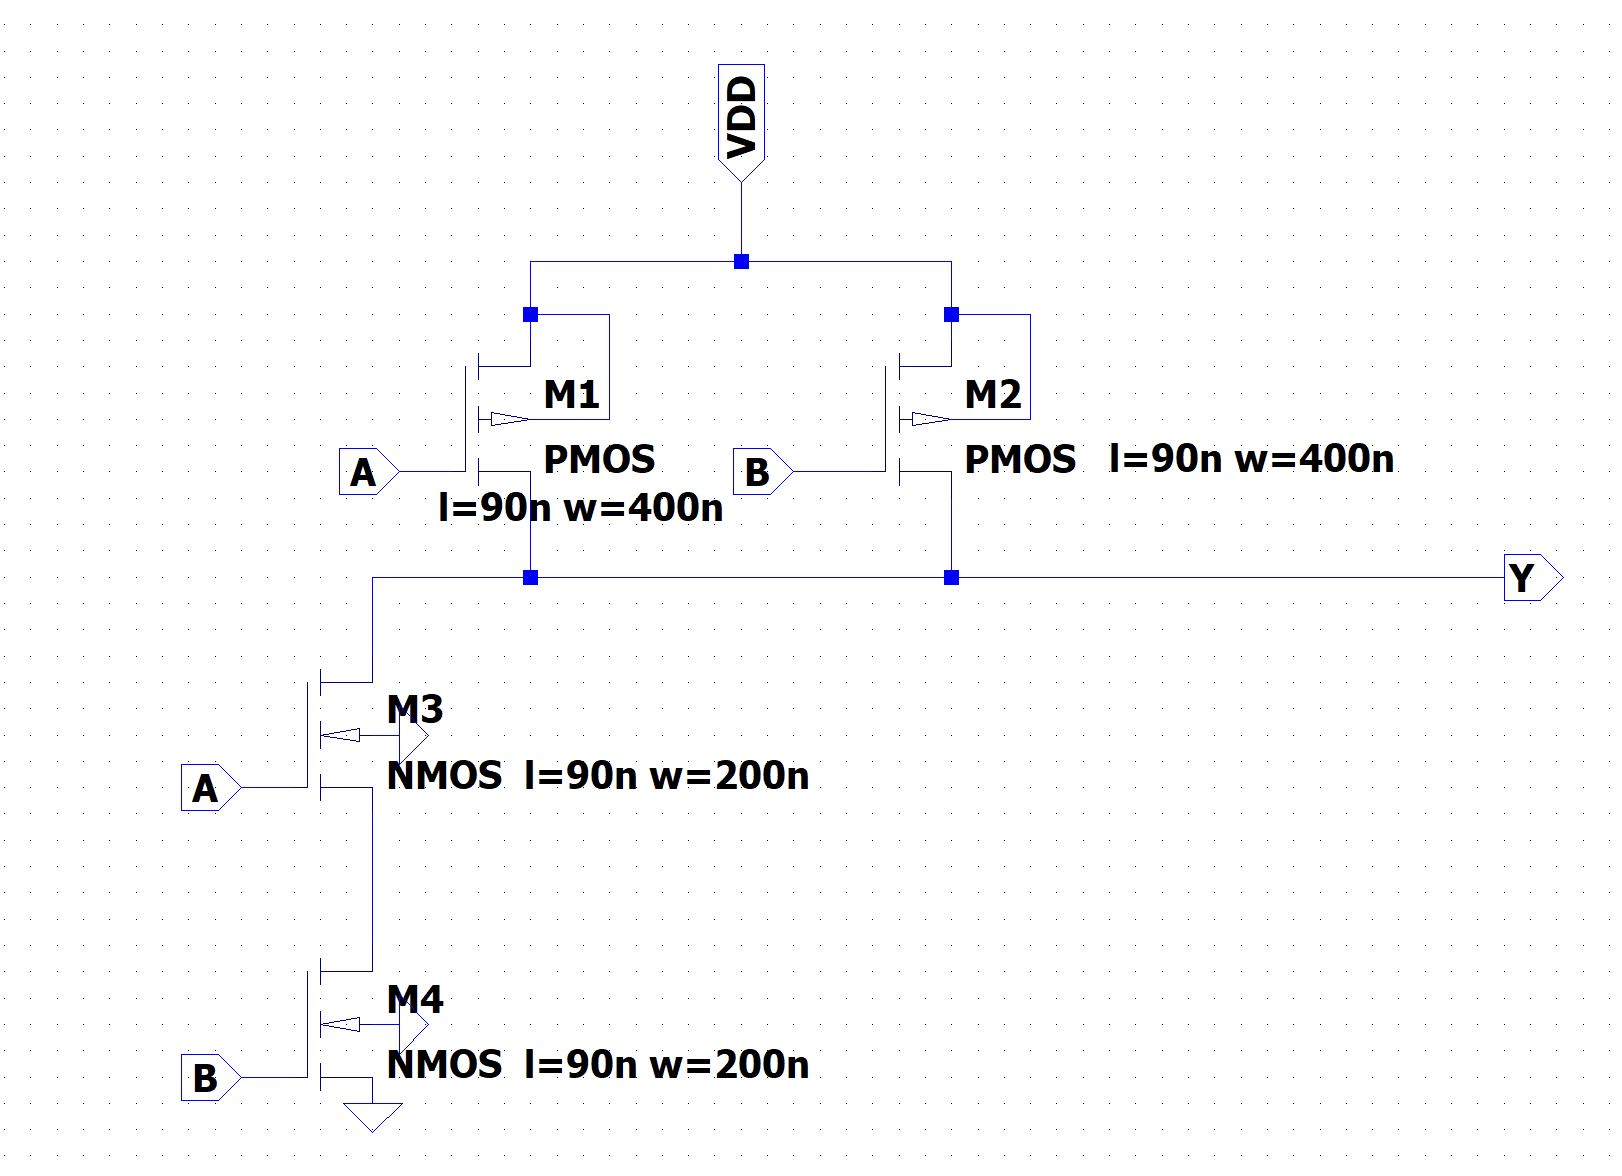
\includegraphics[scale=0.5]{image/ventil.png}
    \caption{Схема разработанного вентиля NAND}
\end{figure}
\subsection{Символ вентиля и схема тестирования}
\begin{figure}[H]
    \centering
    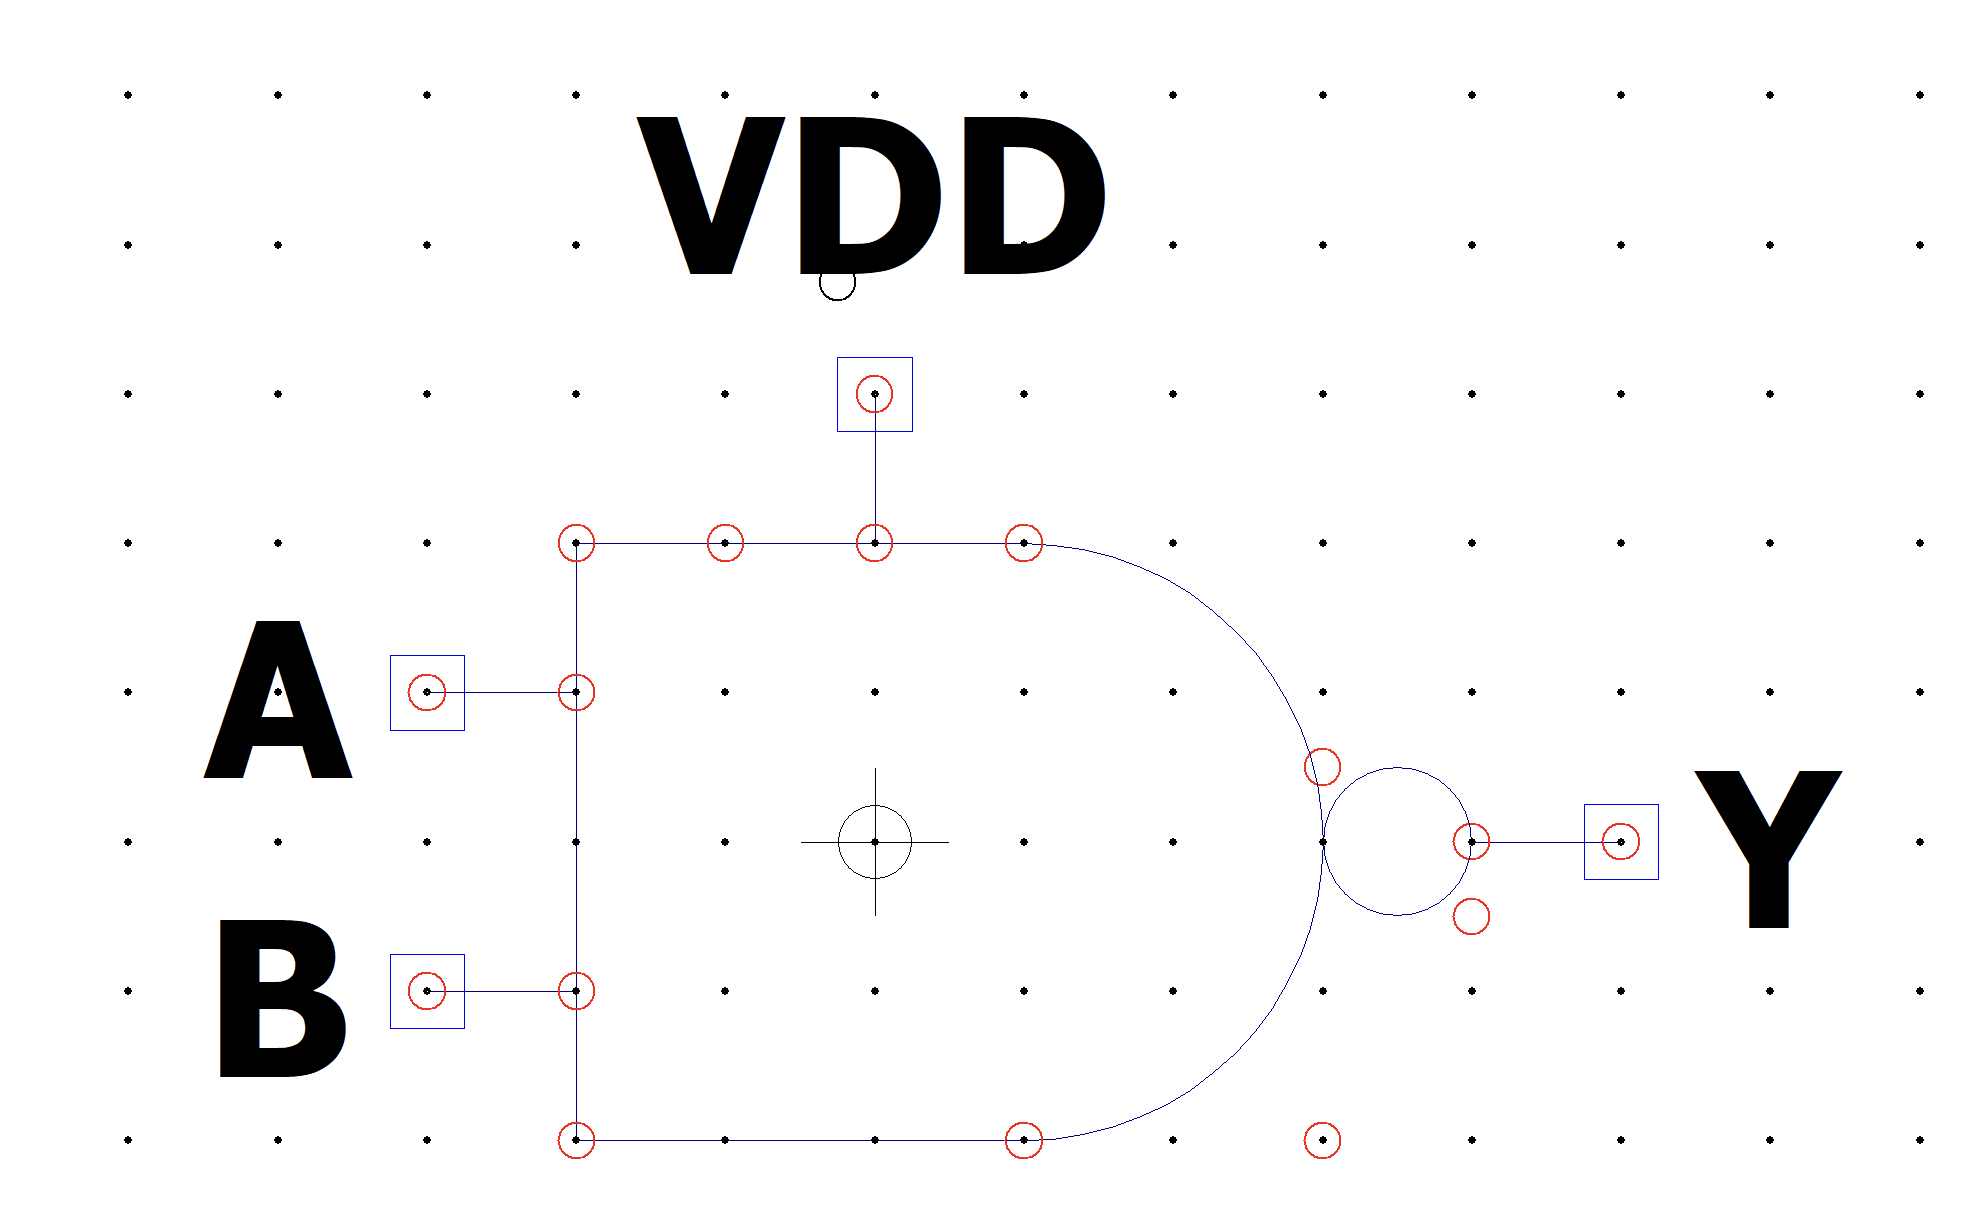
\includegraphics[scale=0.2]{image/symbol.png}
    \caption{Символ вентиля}
\end{figure}
\begin{figure}[H]
    \centering
    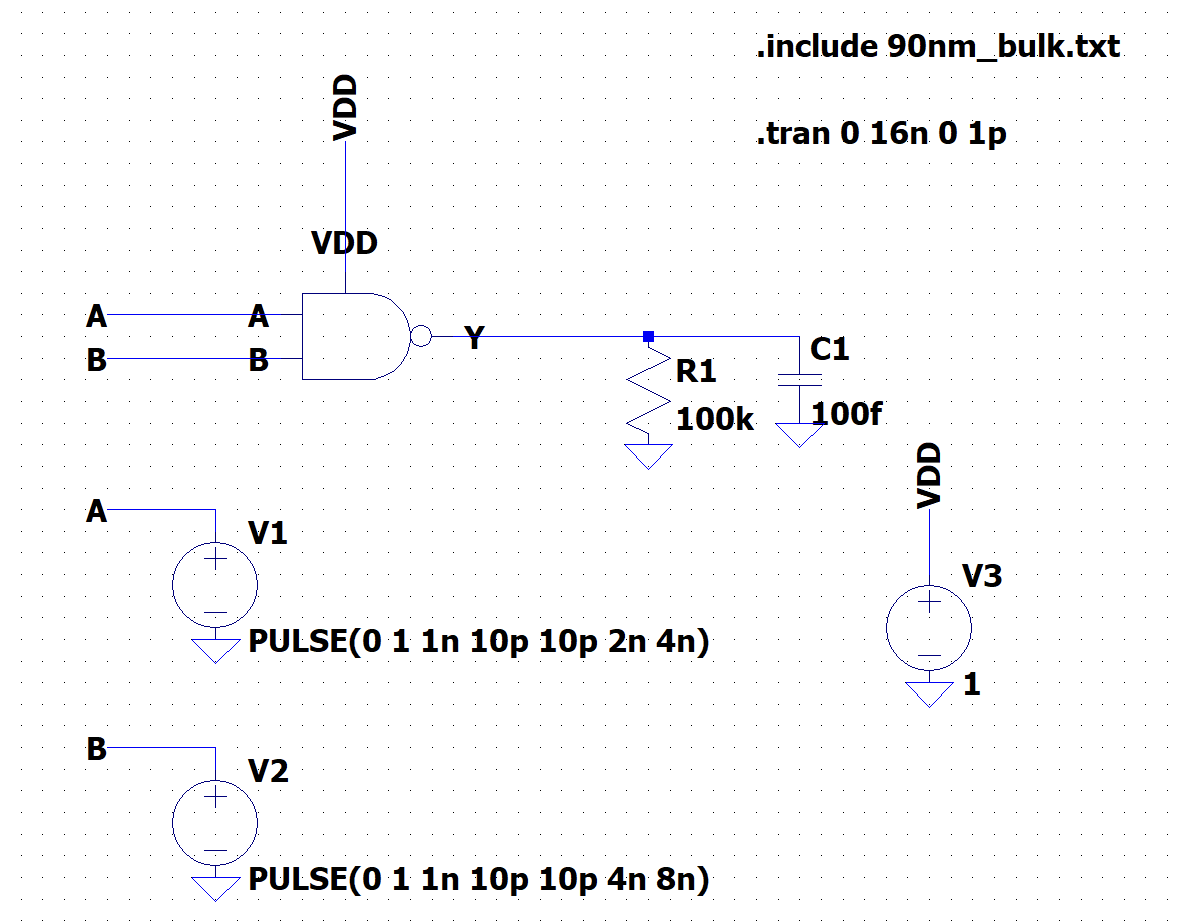
\includegraphics[width=\textwidth]{image/test-circuit.png}
    \caption{Схема тестирования}
\end{figure}
\subsection{Временная диаграмма процесса тестирования вентиля}
\begin{figure}[H]
    \centering
    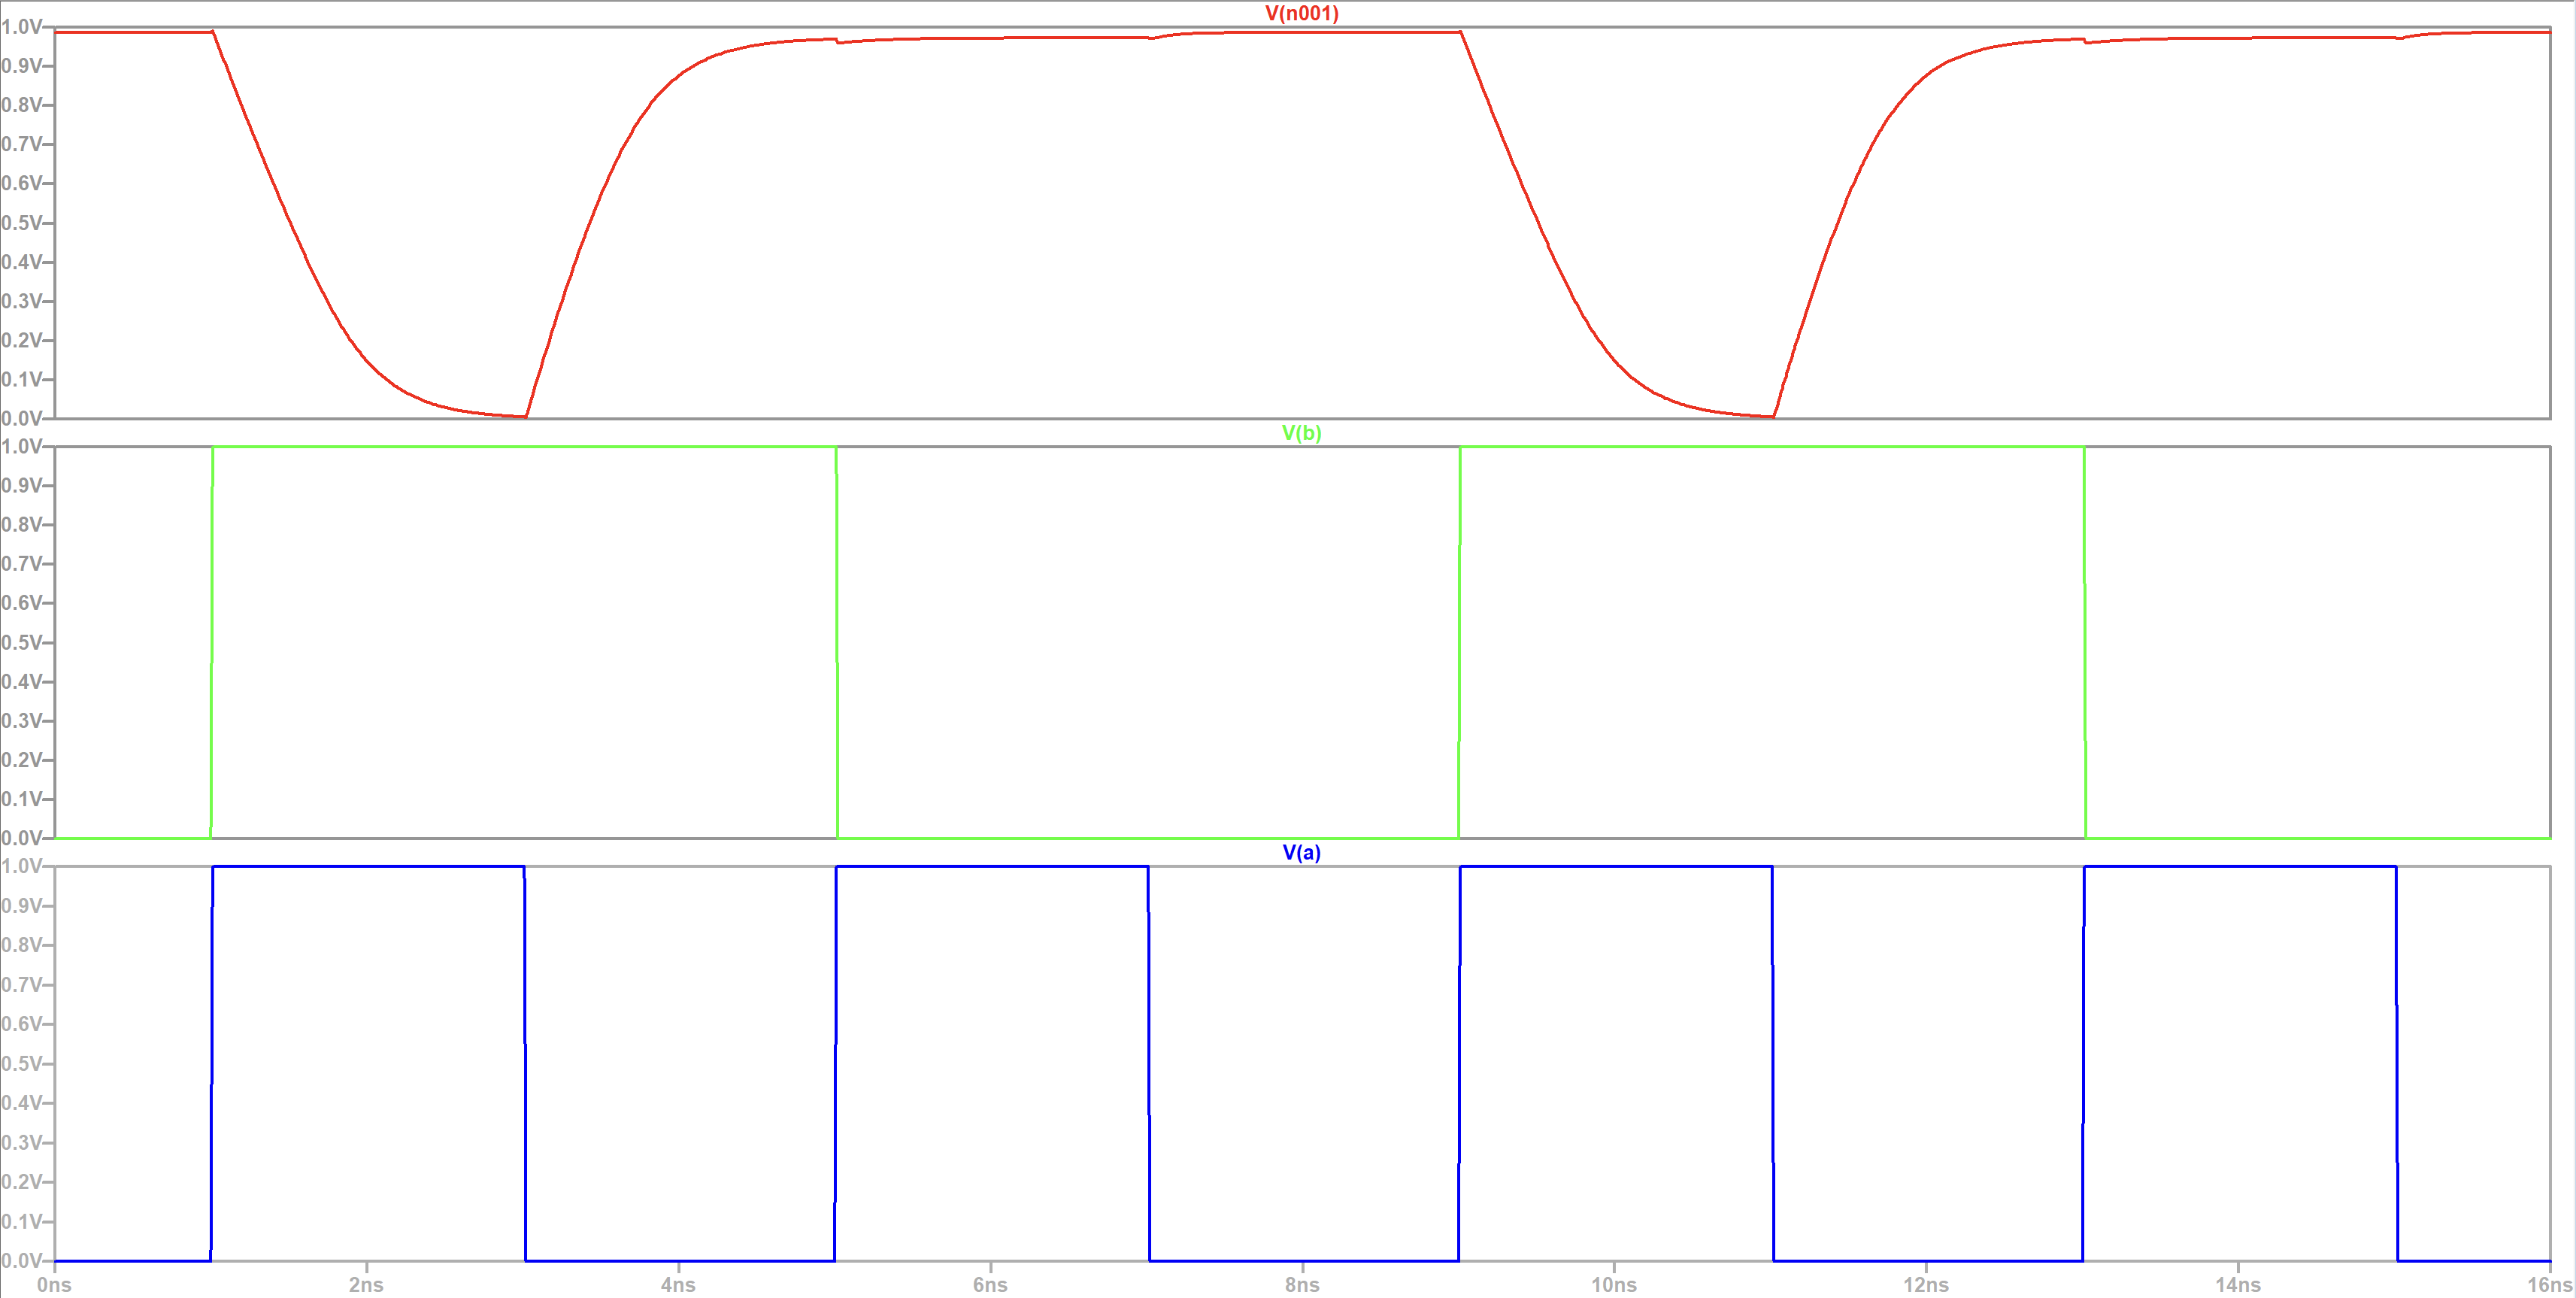
\includegraphics[width=\textwidth]{image/time-diagram.png}
    \caption{Временная диаграмма процесса тестирования вентиля}
\end{figure}
\subsection{Результат измерения задержки распространения сигнала через вентиль}
Задержка распространения - максимальное время от начала изменения входа до момента,
когда все выходы достигнут установившихся значений. Измеряется она между точками
перехода входным и выходным сигналом уровня 50\%.
\begin{figure}[H]
    \centering
    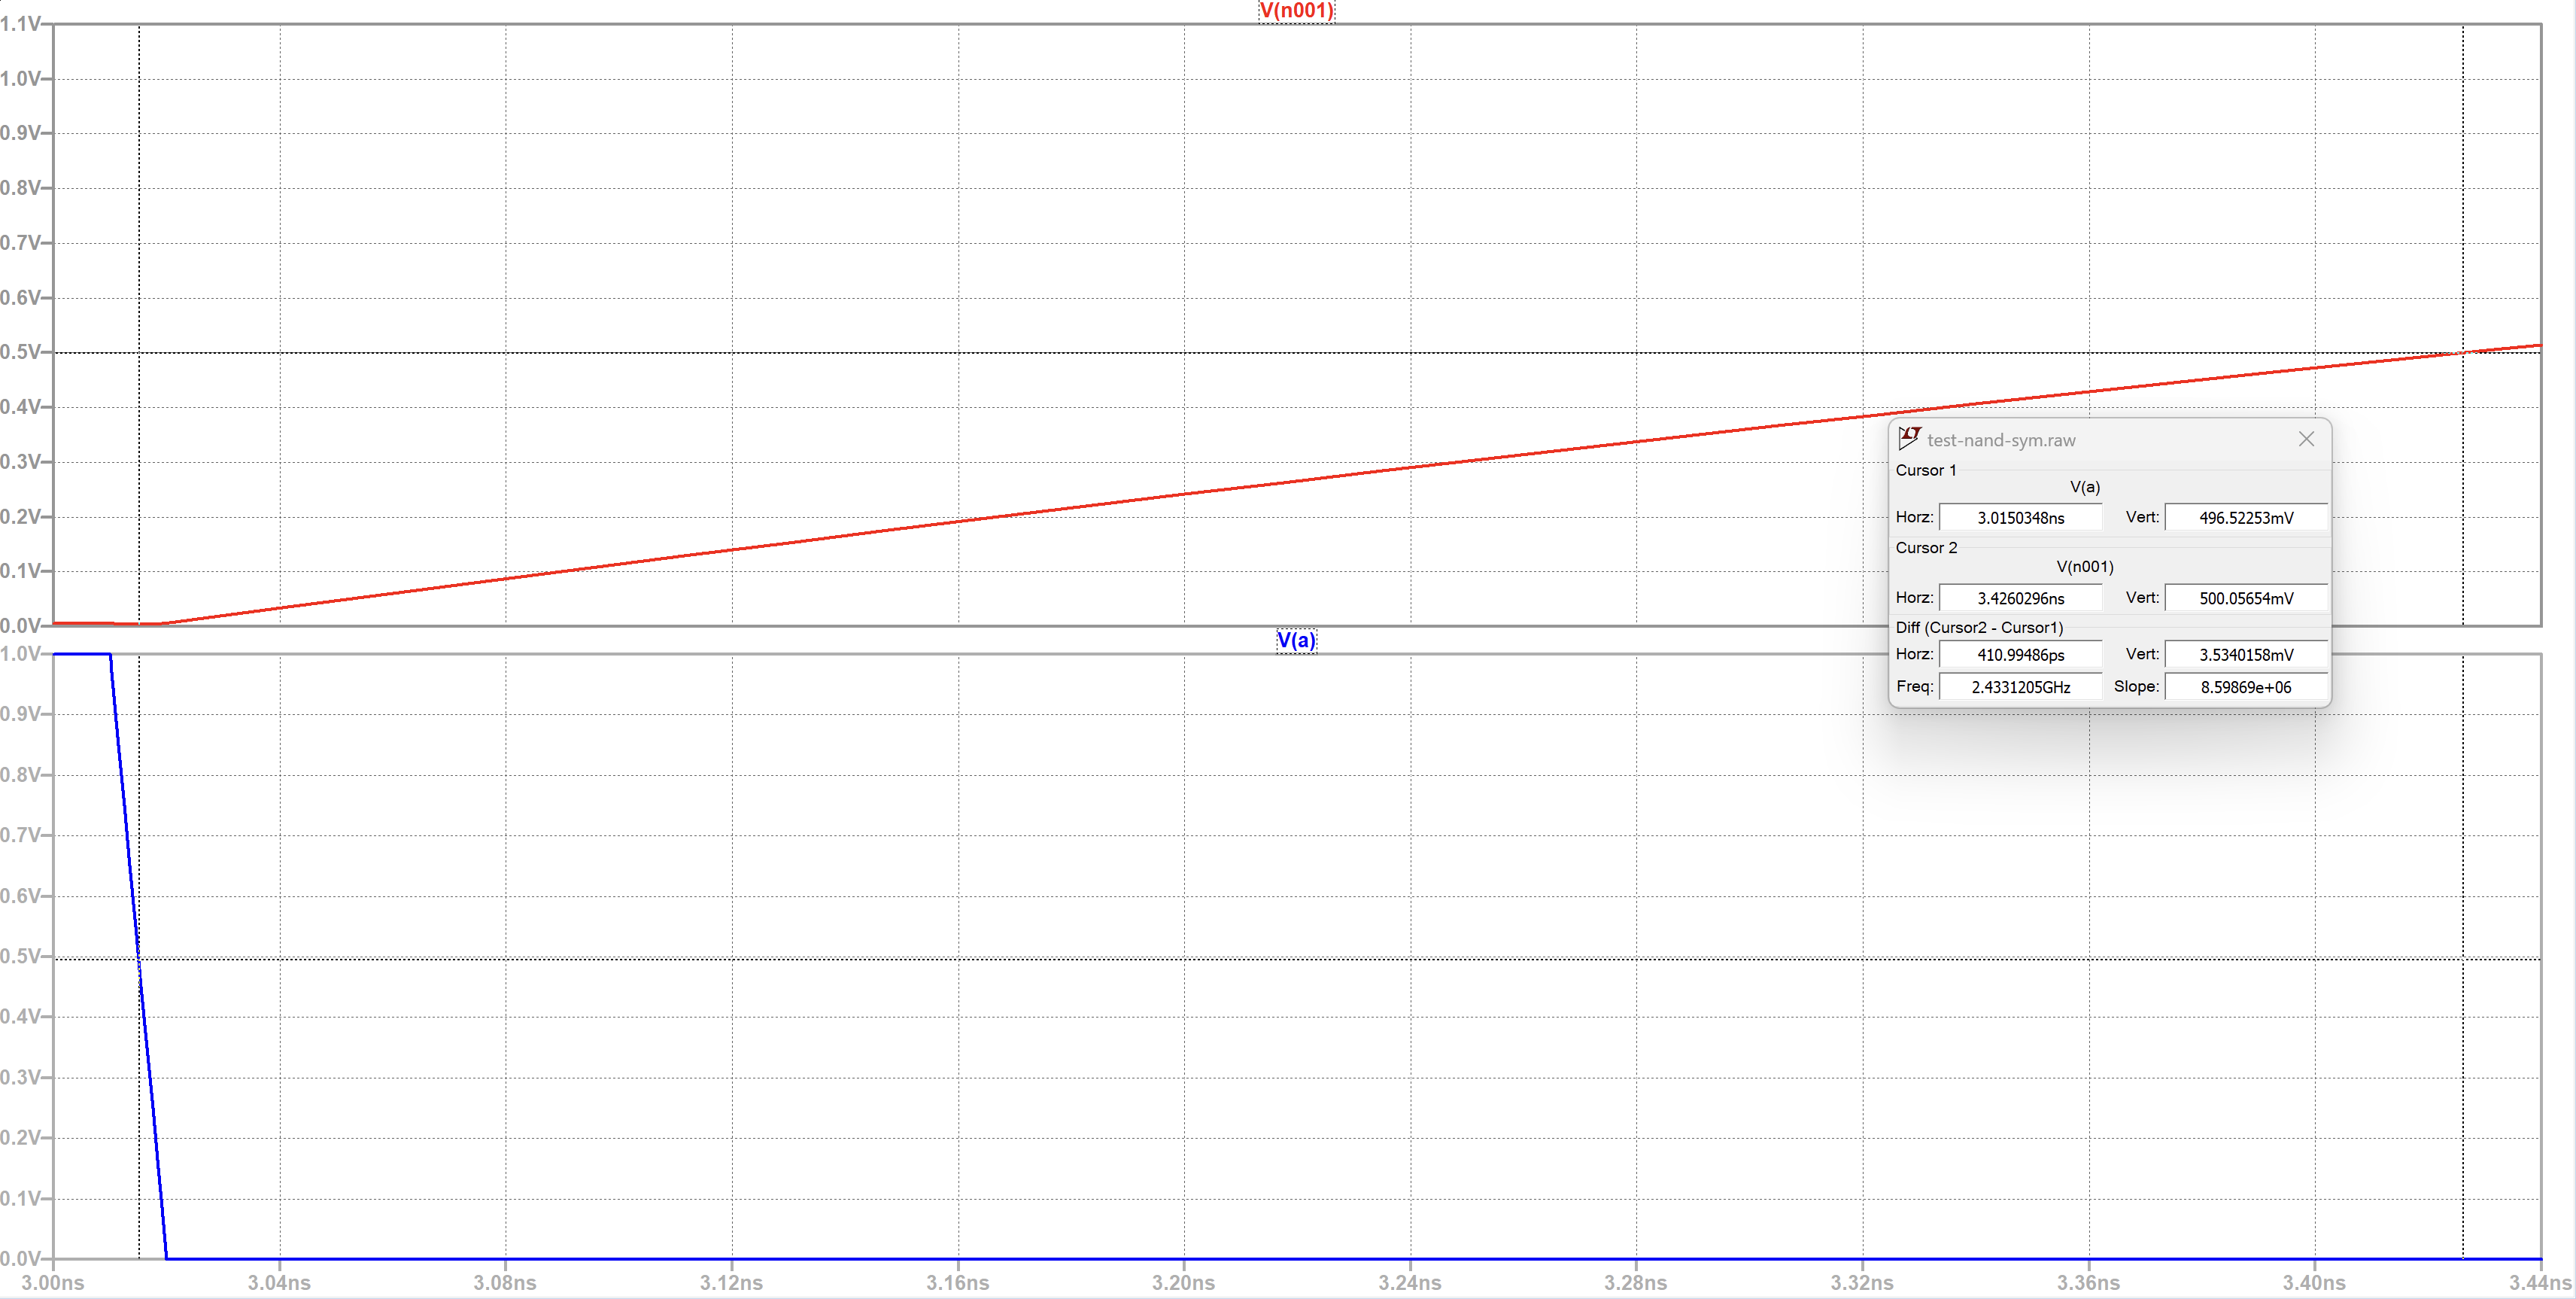
\includegraphics[width=\textwidth]{image/delay0-1.png}
    \caption{Подсчет задержки распространения сигнала для 0-1 на выходе}
\end{figure}
\begin{figure}[H]
    \centering
    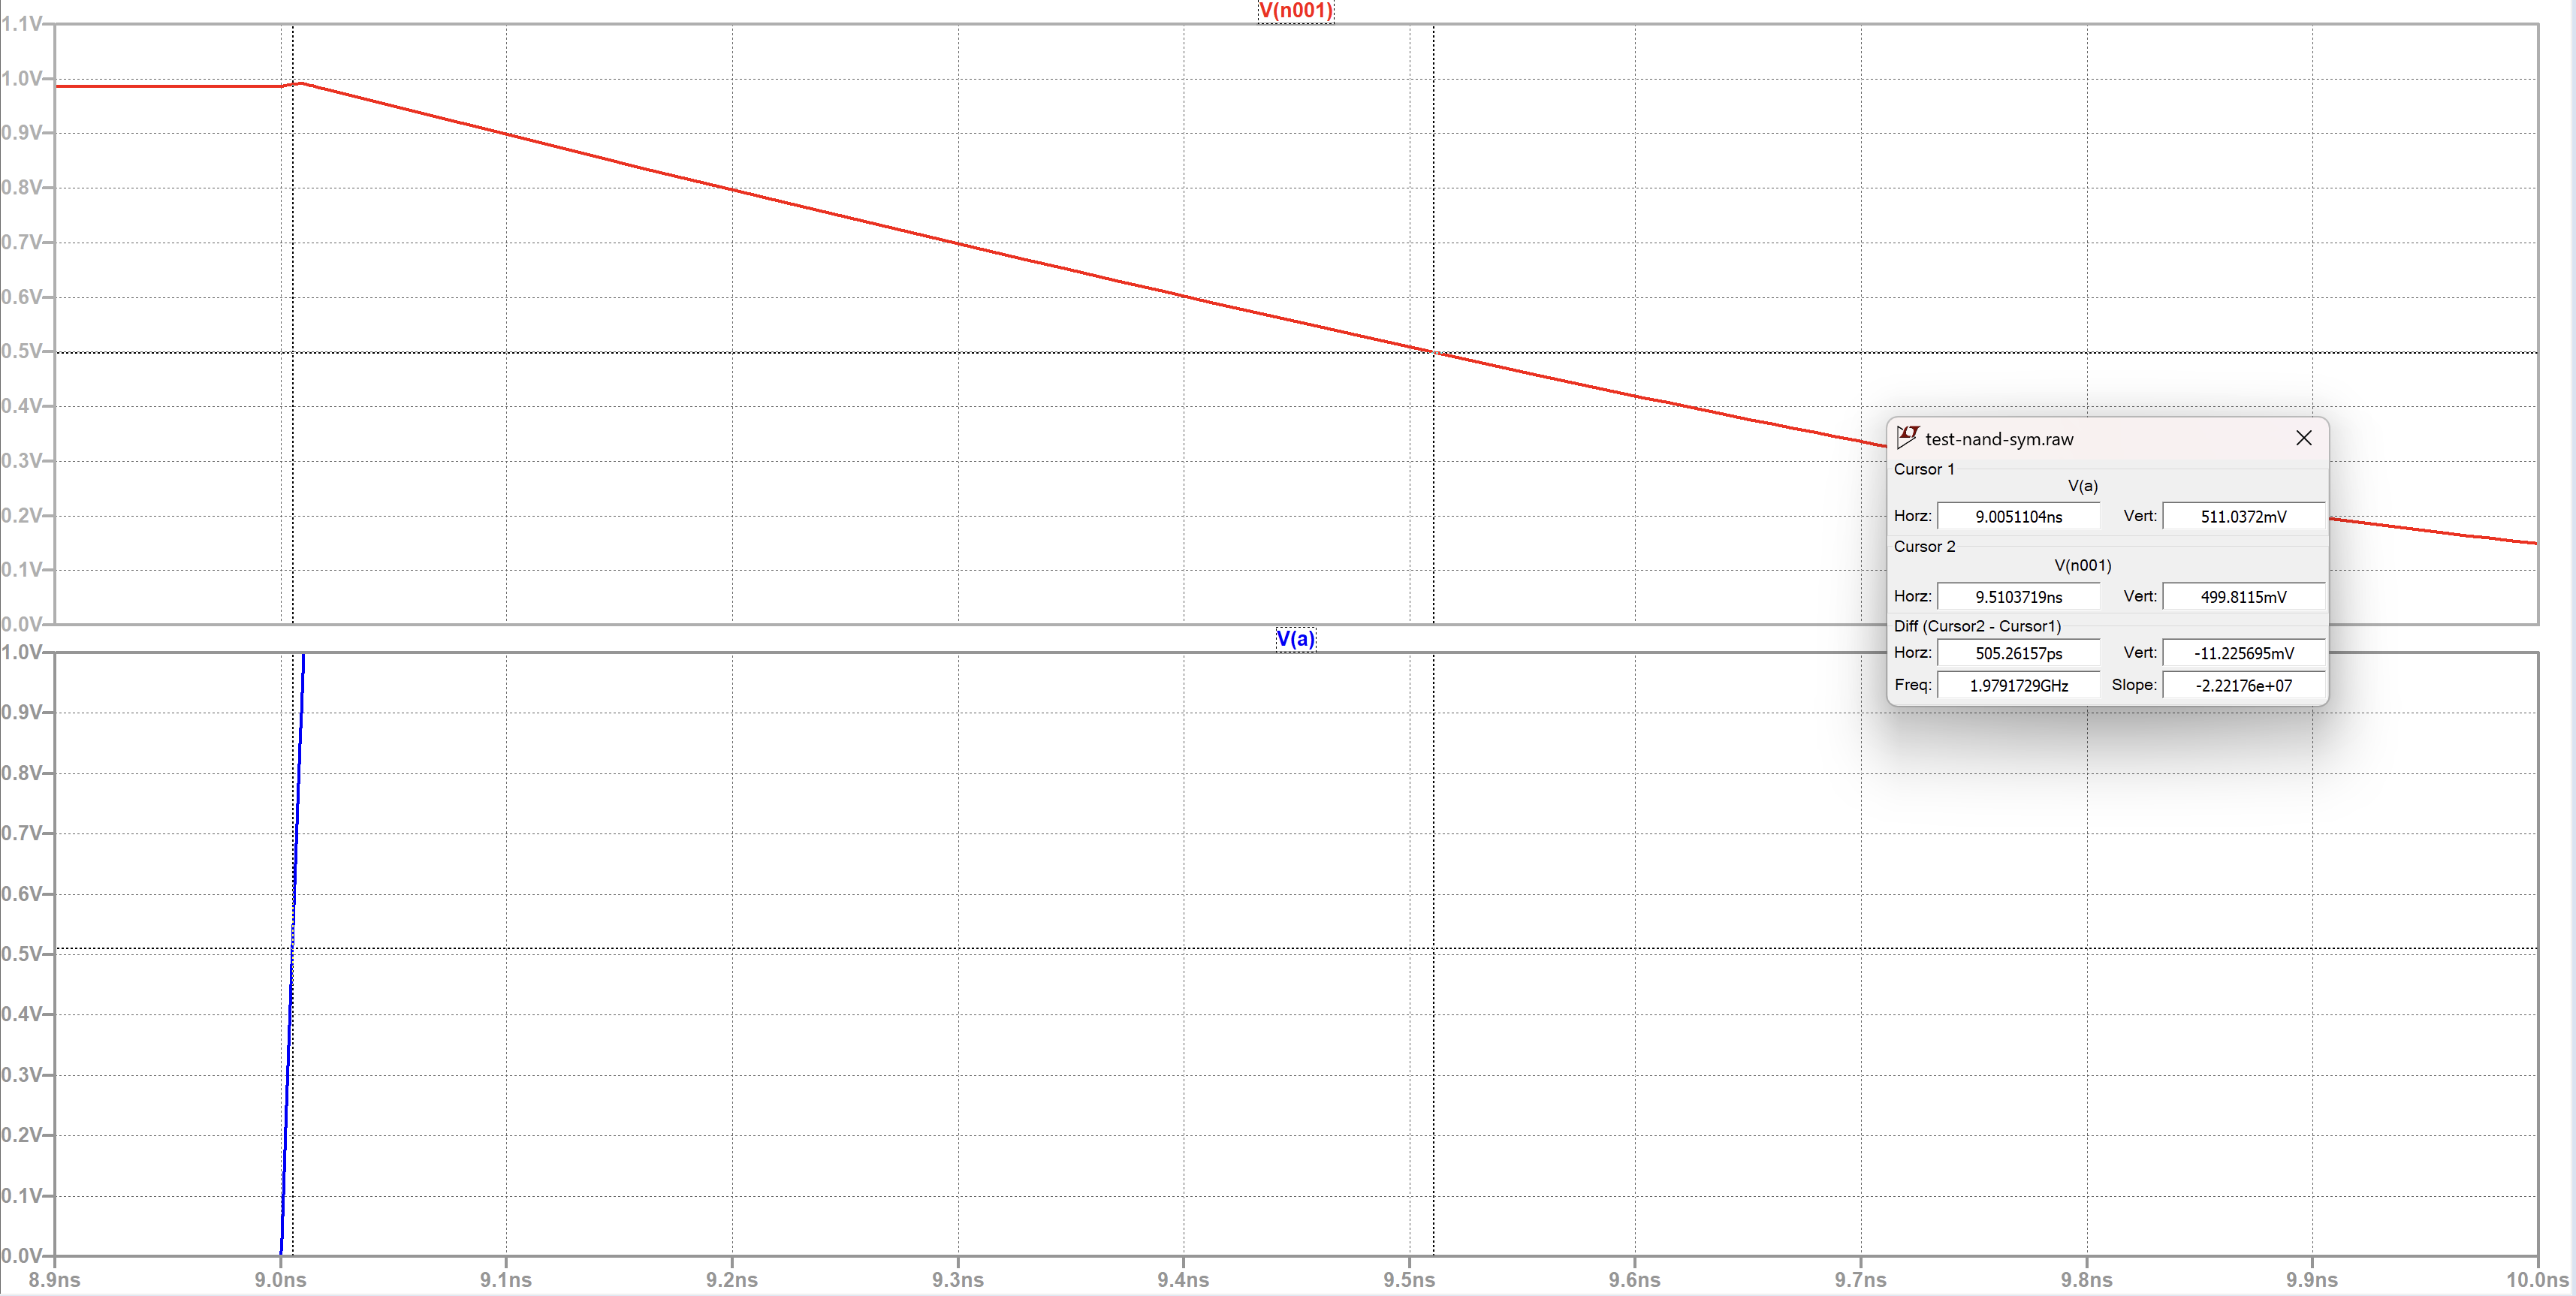
\includegraphics[width=\textwidth]{image/delay1-0.png}
    \caption{Подсчет задержки распространения сигнала для 1-0 на выходе}
\end{figure}
$$
    t_{pd} = t_2 - t_1 = 3.426 - 3.015 = 0.411 \text{нс} - \text{задержка распространения сигнала для 0-1 на выходе}
$$
$$
    t_{pd} = t_2 - t_1 = 9.510 - 9.005 = 0.505 \text{нс} - \text{задержка распространения сигнала для 1-0 на выходе}
$$
\subsection{Максимальная частота работы вентиля}
$$
    \nu_{\text{спада}} = \frac{1}{t_{10}} = \frac{1}{0.411} = 2.267 \text{ГГц}
$$
$$
    \nu_{\text{фронта}} = \frac{1}{t_{01}} = \frac{1}{0.505} = 1.980 \text{ГГц}
$$
Тогда максимальная частота работы вентиля:
$$
\nu_{\max} = \min(\nu_{\text{спада}}, \nu_{\text{фронта}}) = \min(2.267, 1.980 ) = 2.267 \text{ГГц}
$$
Видим, что это на это влияют конденсатор и резистор. Если начем изменять значения резистора, то мы заметим, что чем меньше его емкость, тем меньше задержка.
\begin{figure}[H]
    \centering
    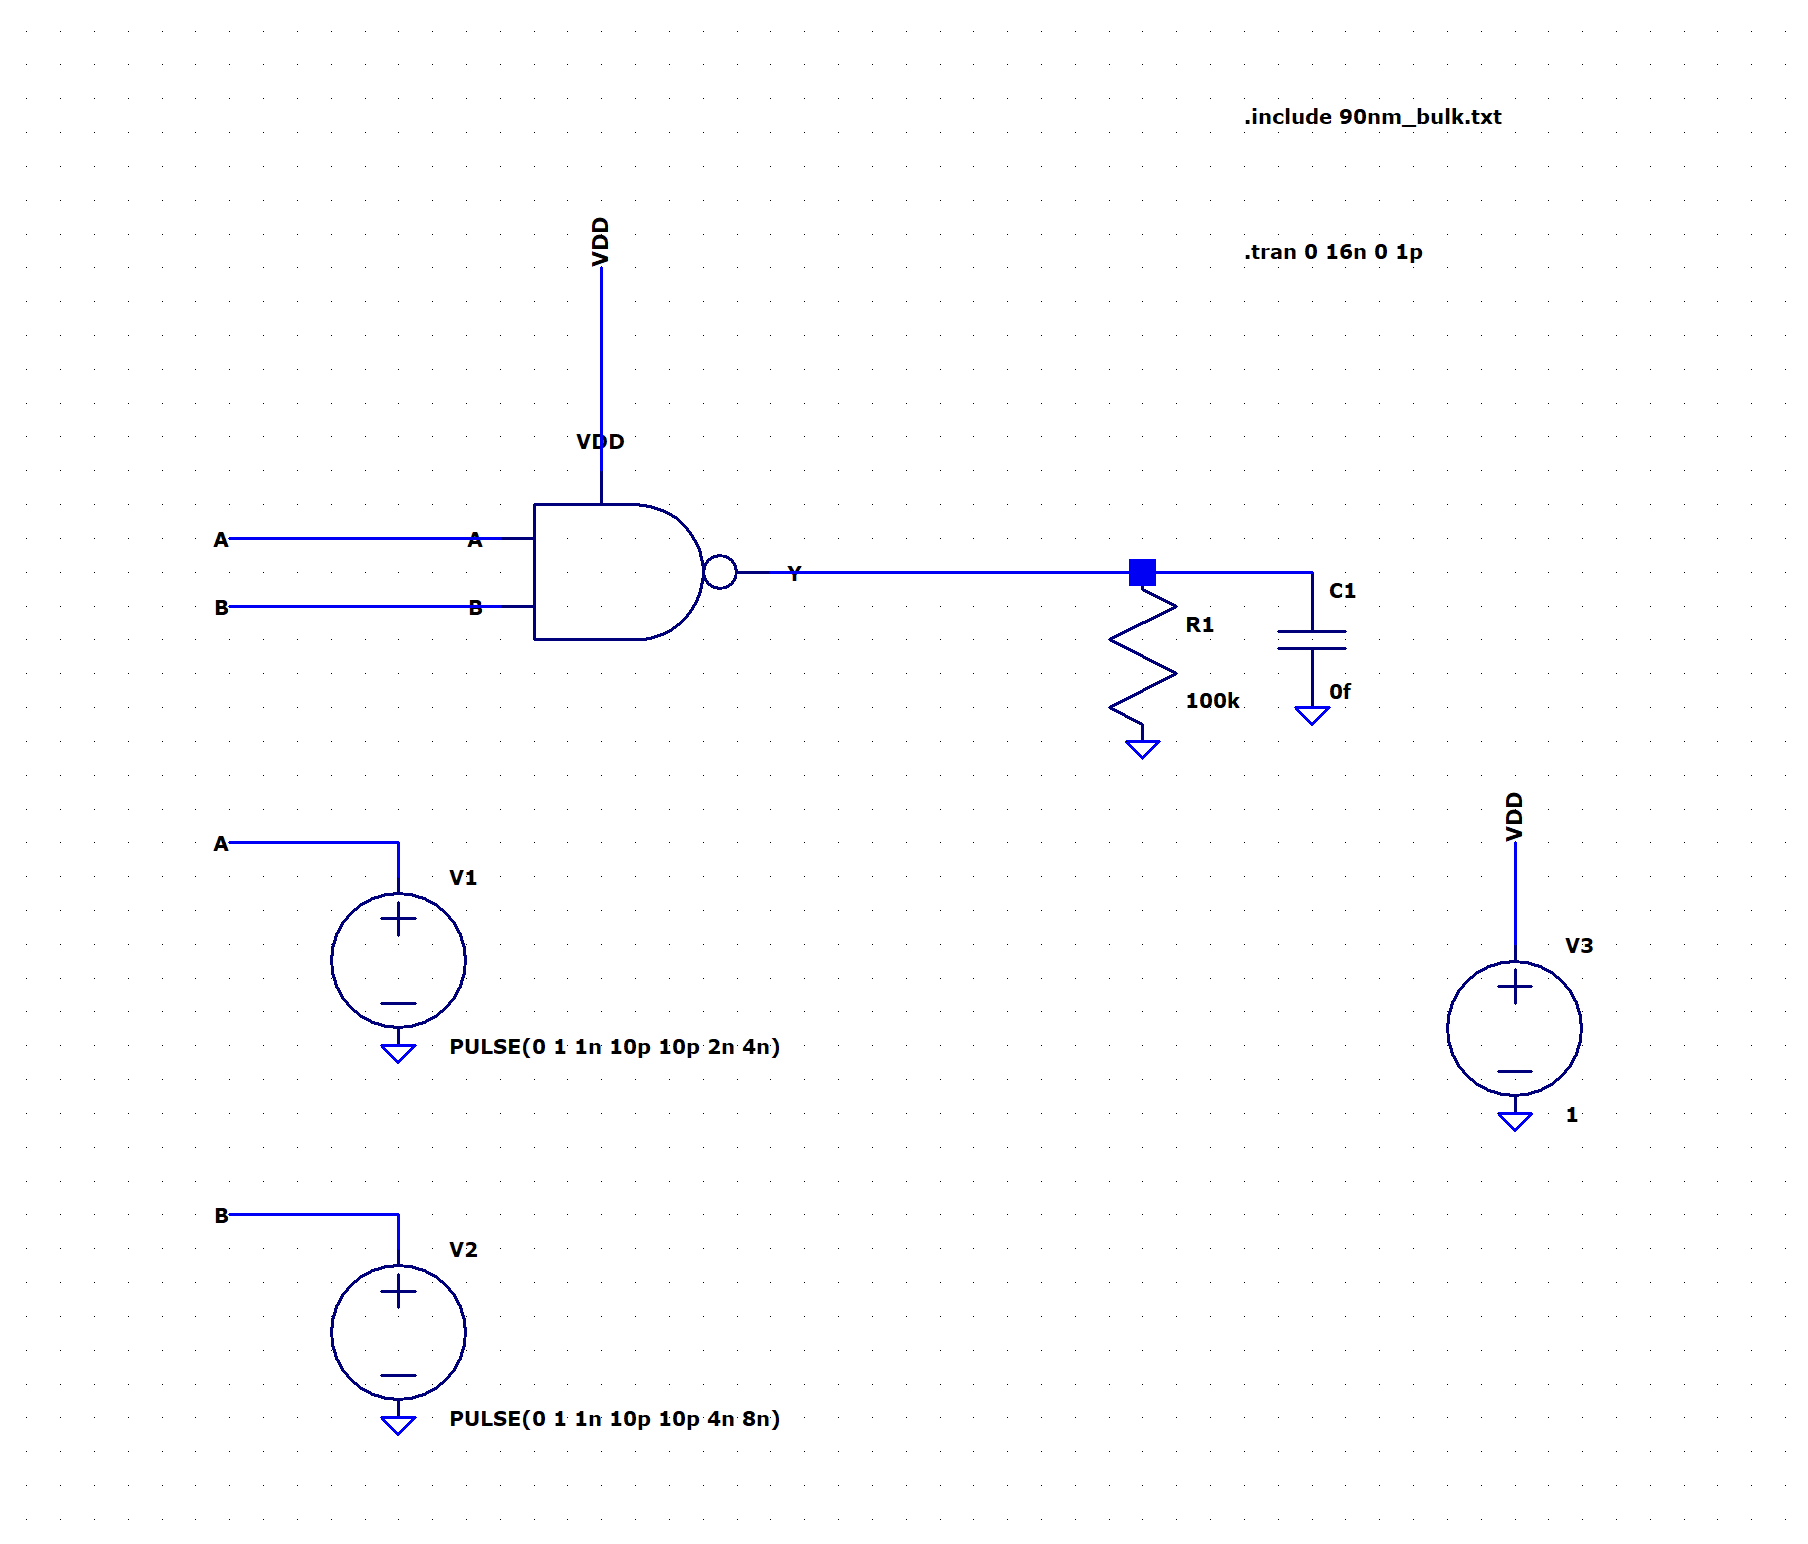
\includegraphics[width=\textwidth]{image/schema-1.png}
    \caption{Берем кондексатор равный 0 фемптофаррад }
\end{figure}
\begin{figure}[H]
    \centering
    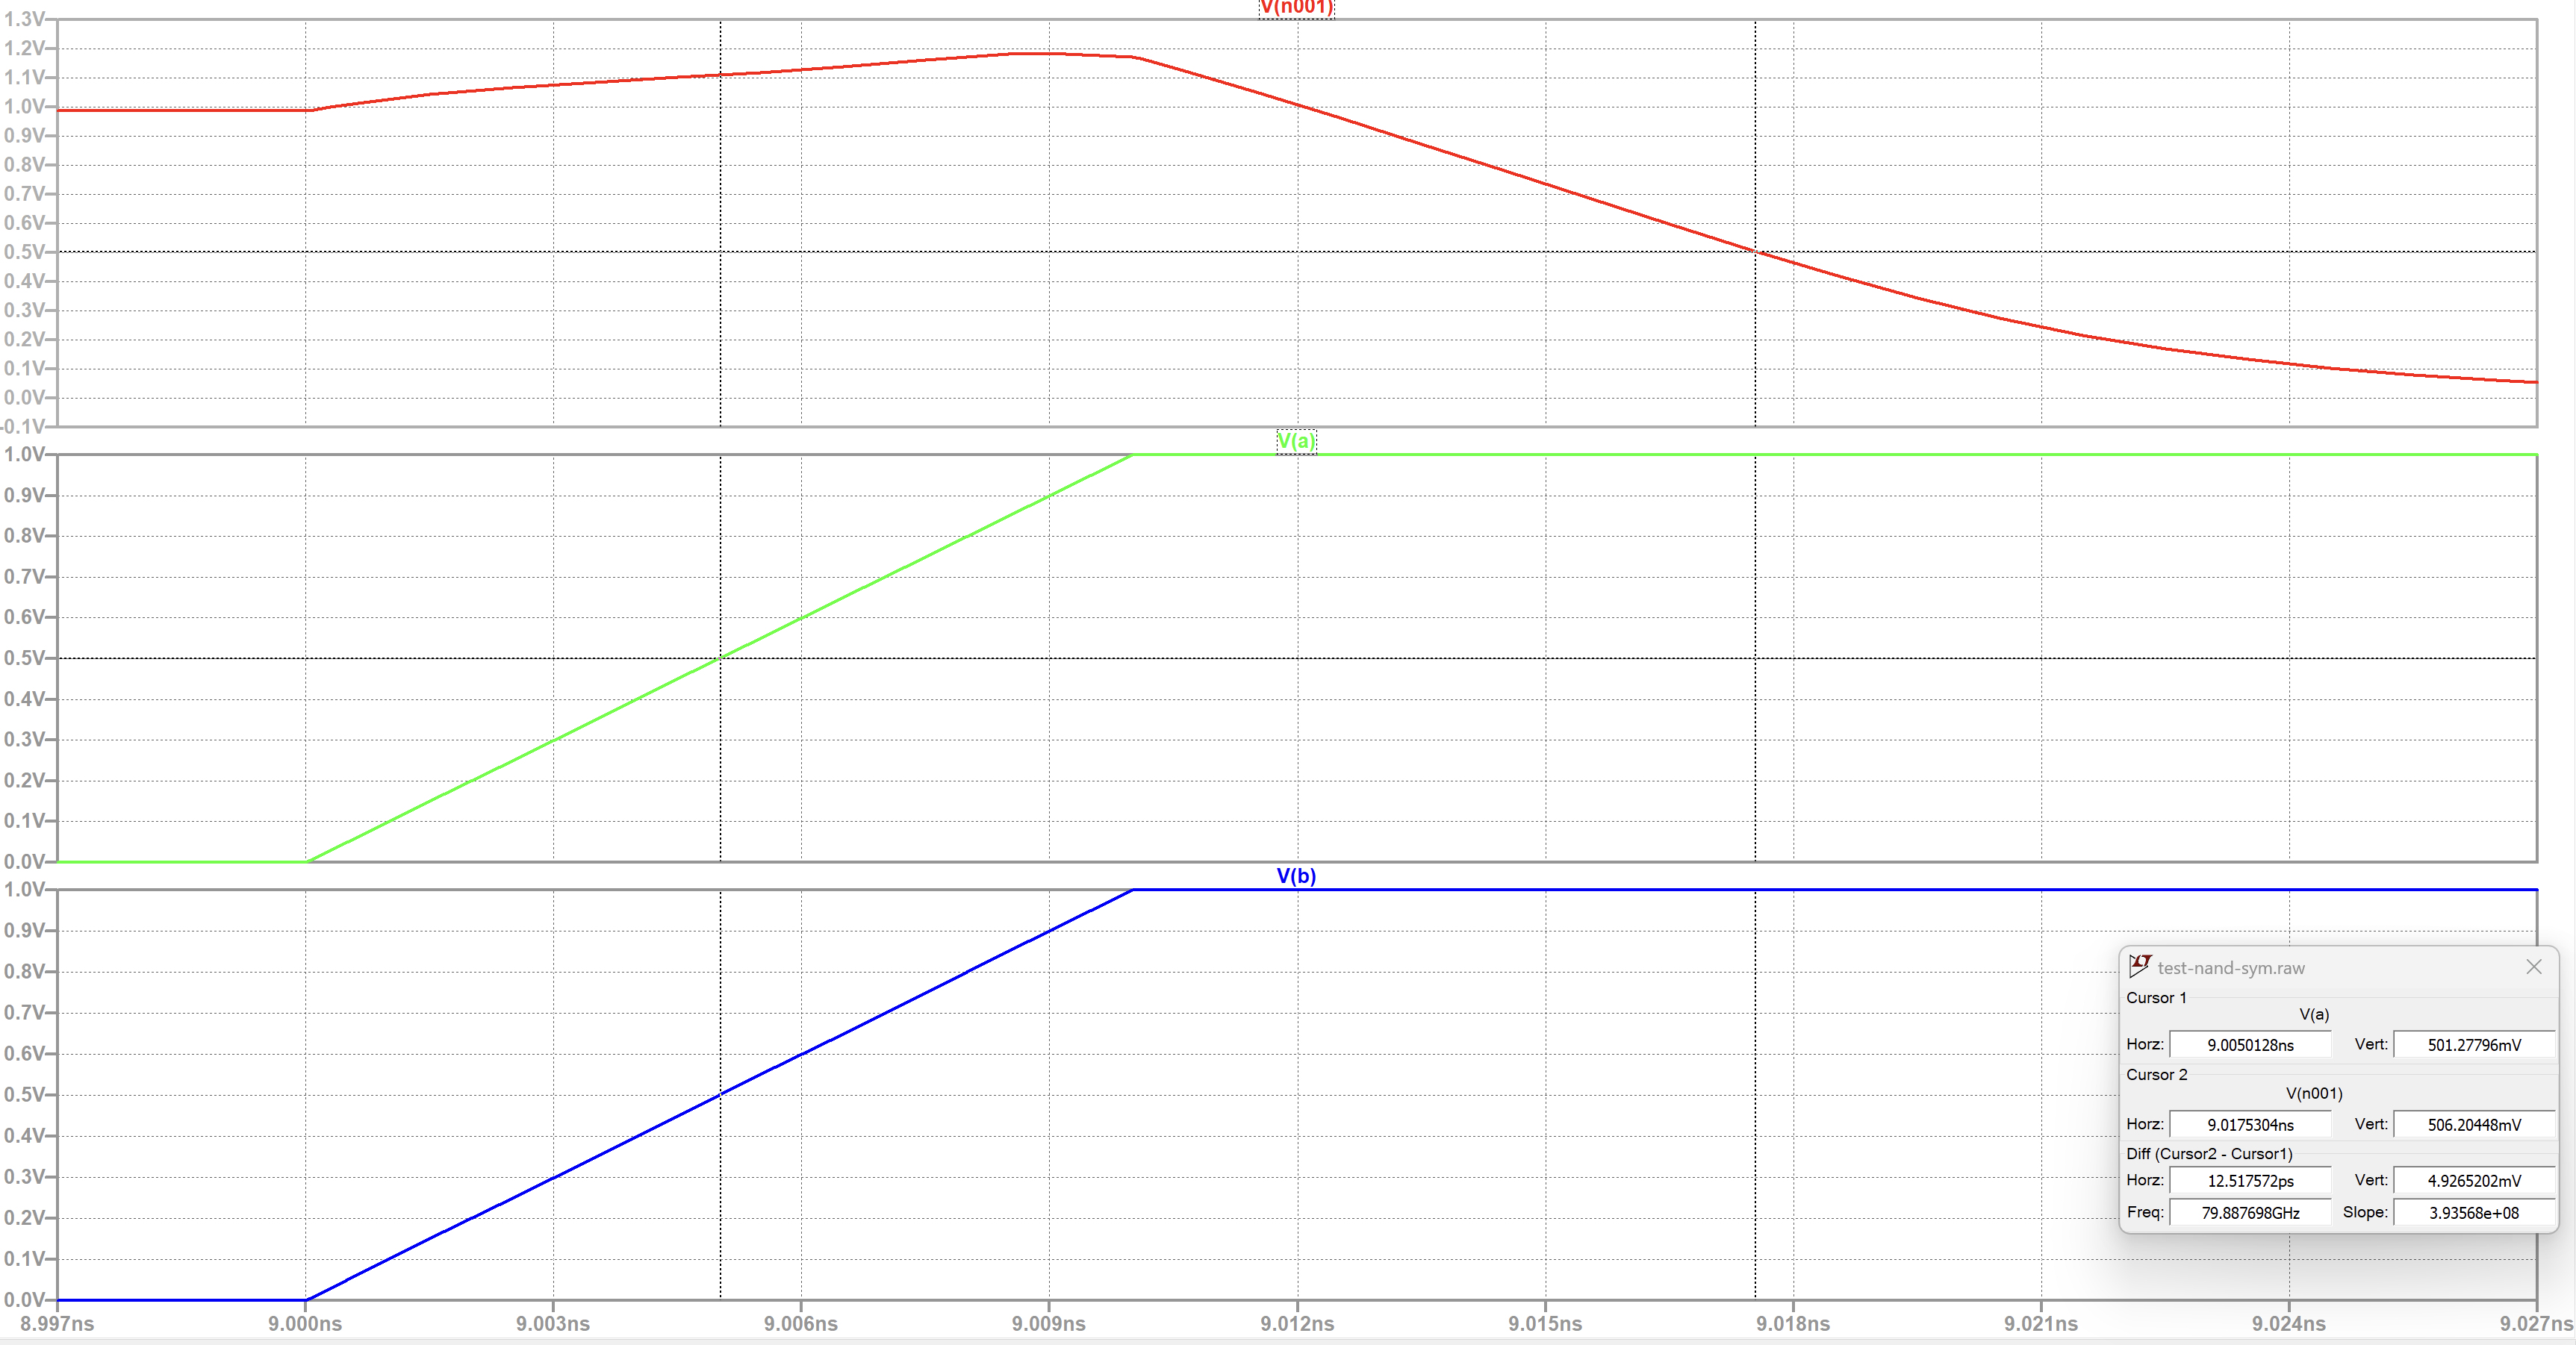
\includegraphics[width=\textwidth]{image/fall.png}
    \caption{Подсчет задержки распространения сигнала для 0-1 на выходе}
\end{figure}
\begin{figure}[H]
    \centering
    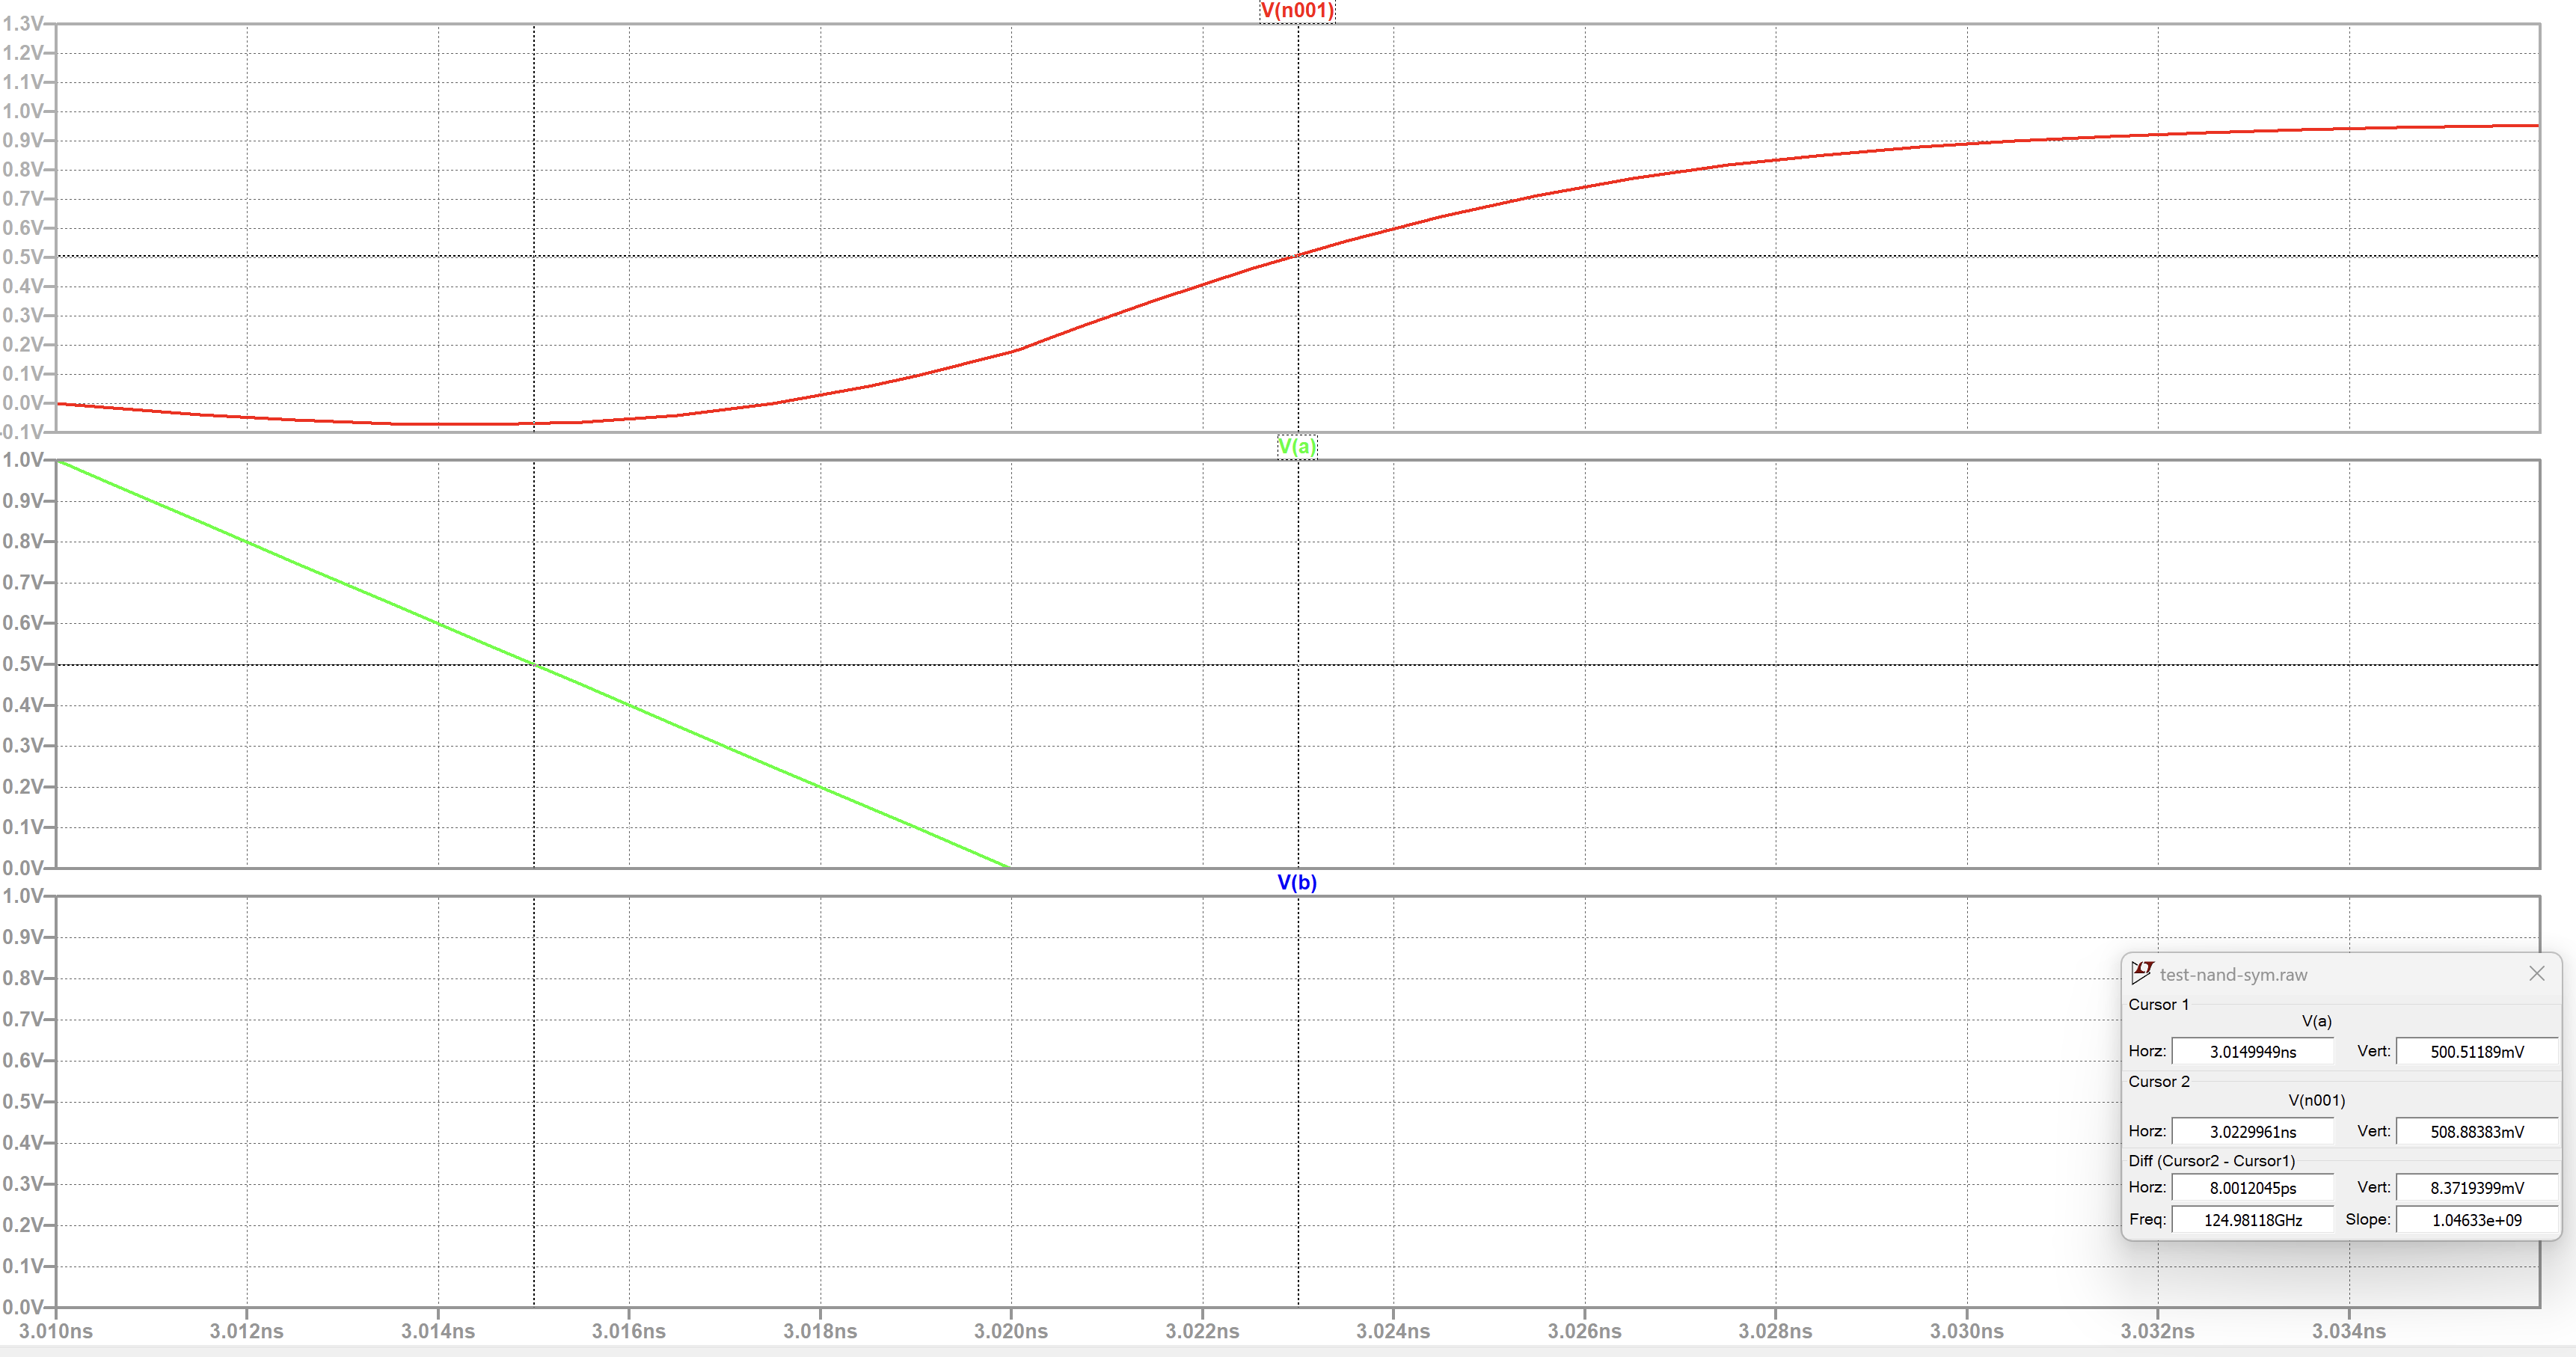
\includegraphics[width=\textwidth]{image/rise.png}
    \caption{Подсчет задержки распространения сигнала для 1-0 на выходе}
\end{figure}
$$
    t_{pd} = t_2 - t_1 = 9 \text{ps} - \text{задержка распространения сигнала для 0-1 на выходе}
$$
$$
    t_{pd} = t_2 - t_1 = 12 \text{ps} - \text{задержка распространения сигнала для 1-0 на выходе}
$$
$$
    \nu_{\text{спада}} = \frac{1}{t_{10}} = \frac{1}{9} = 110 \text{ГГц}
$$
$$
    \nu_{\text{фронта}} = \frac{1}{t_{01}} = \frac{1}{12} = 83\text{ГГц}
$$
Тогда максимальная частота работы вентиля:
$$
\nu_{\max} = \min(\nu_{\text{спада}}, \nu_{\text{фронта}}) = \min(110, 83 ) = 83 \text{ГГц}
$$

\subsection{Постройте БОЭ на базе созданного вентиля согласно варианту задания.}
Полный четырех разрядный компаратор.
$$
\begin{aligned}
    & (A = B)- \overline{\bar{A} B \vee A \bar{B}}=\overline{\overline{\overline{\bar{A} B} \wedge \overline{\bar{A} \bar{B}}}}
= \overline{\overline{(\bar{A} \mid B)(A \mid \bar{B})}}=\overline{(\bar{A} \mid B) \mid(A \mid \bar{B})}\\
& (A<B)-\bar{A} B=\overline{\overline{\bar{A} B}}=\overline{(\bar{A} \mid B)} \\
& (A>B)-A \bar{B}=\overline{\overline{A B}}=(\overline{A \mid \bar{B}})\\
& \bar{A} = (A \mid A)
\end{aligned}
$$
\begin{figure}[H]
    \centering
    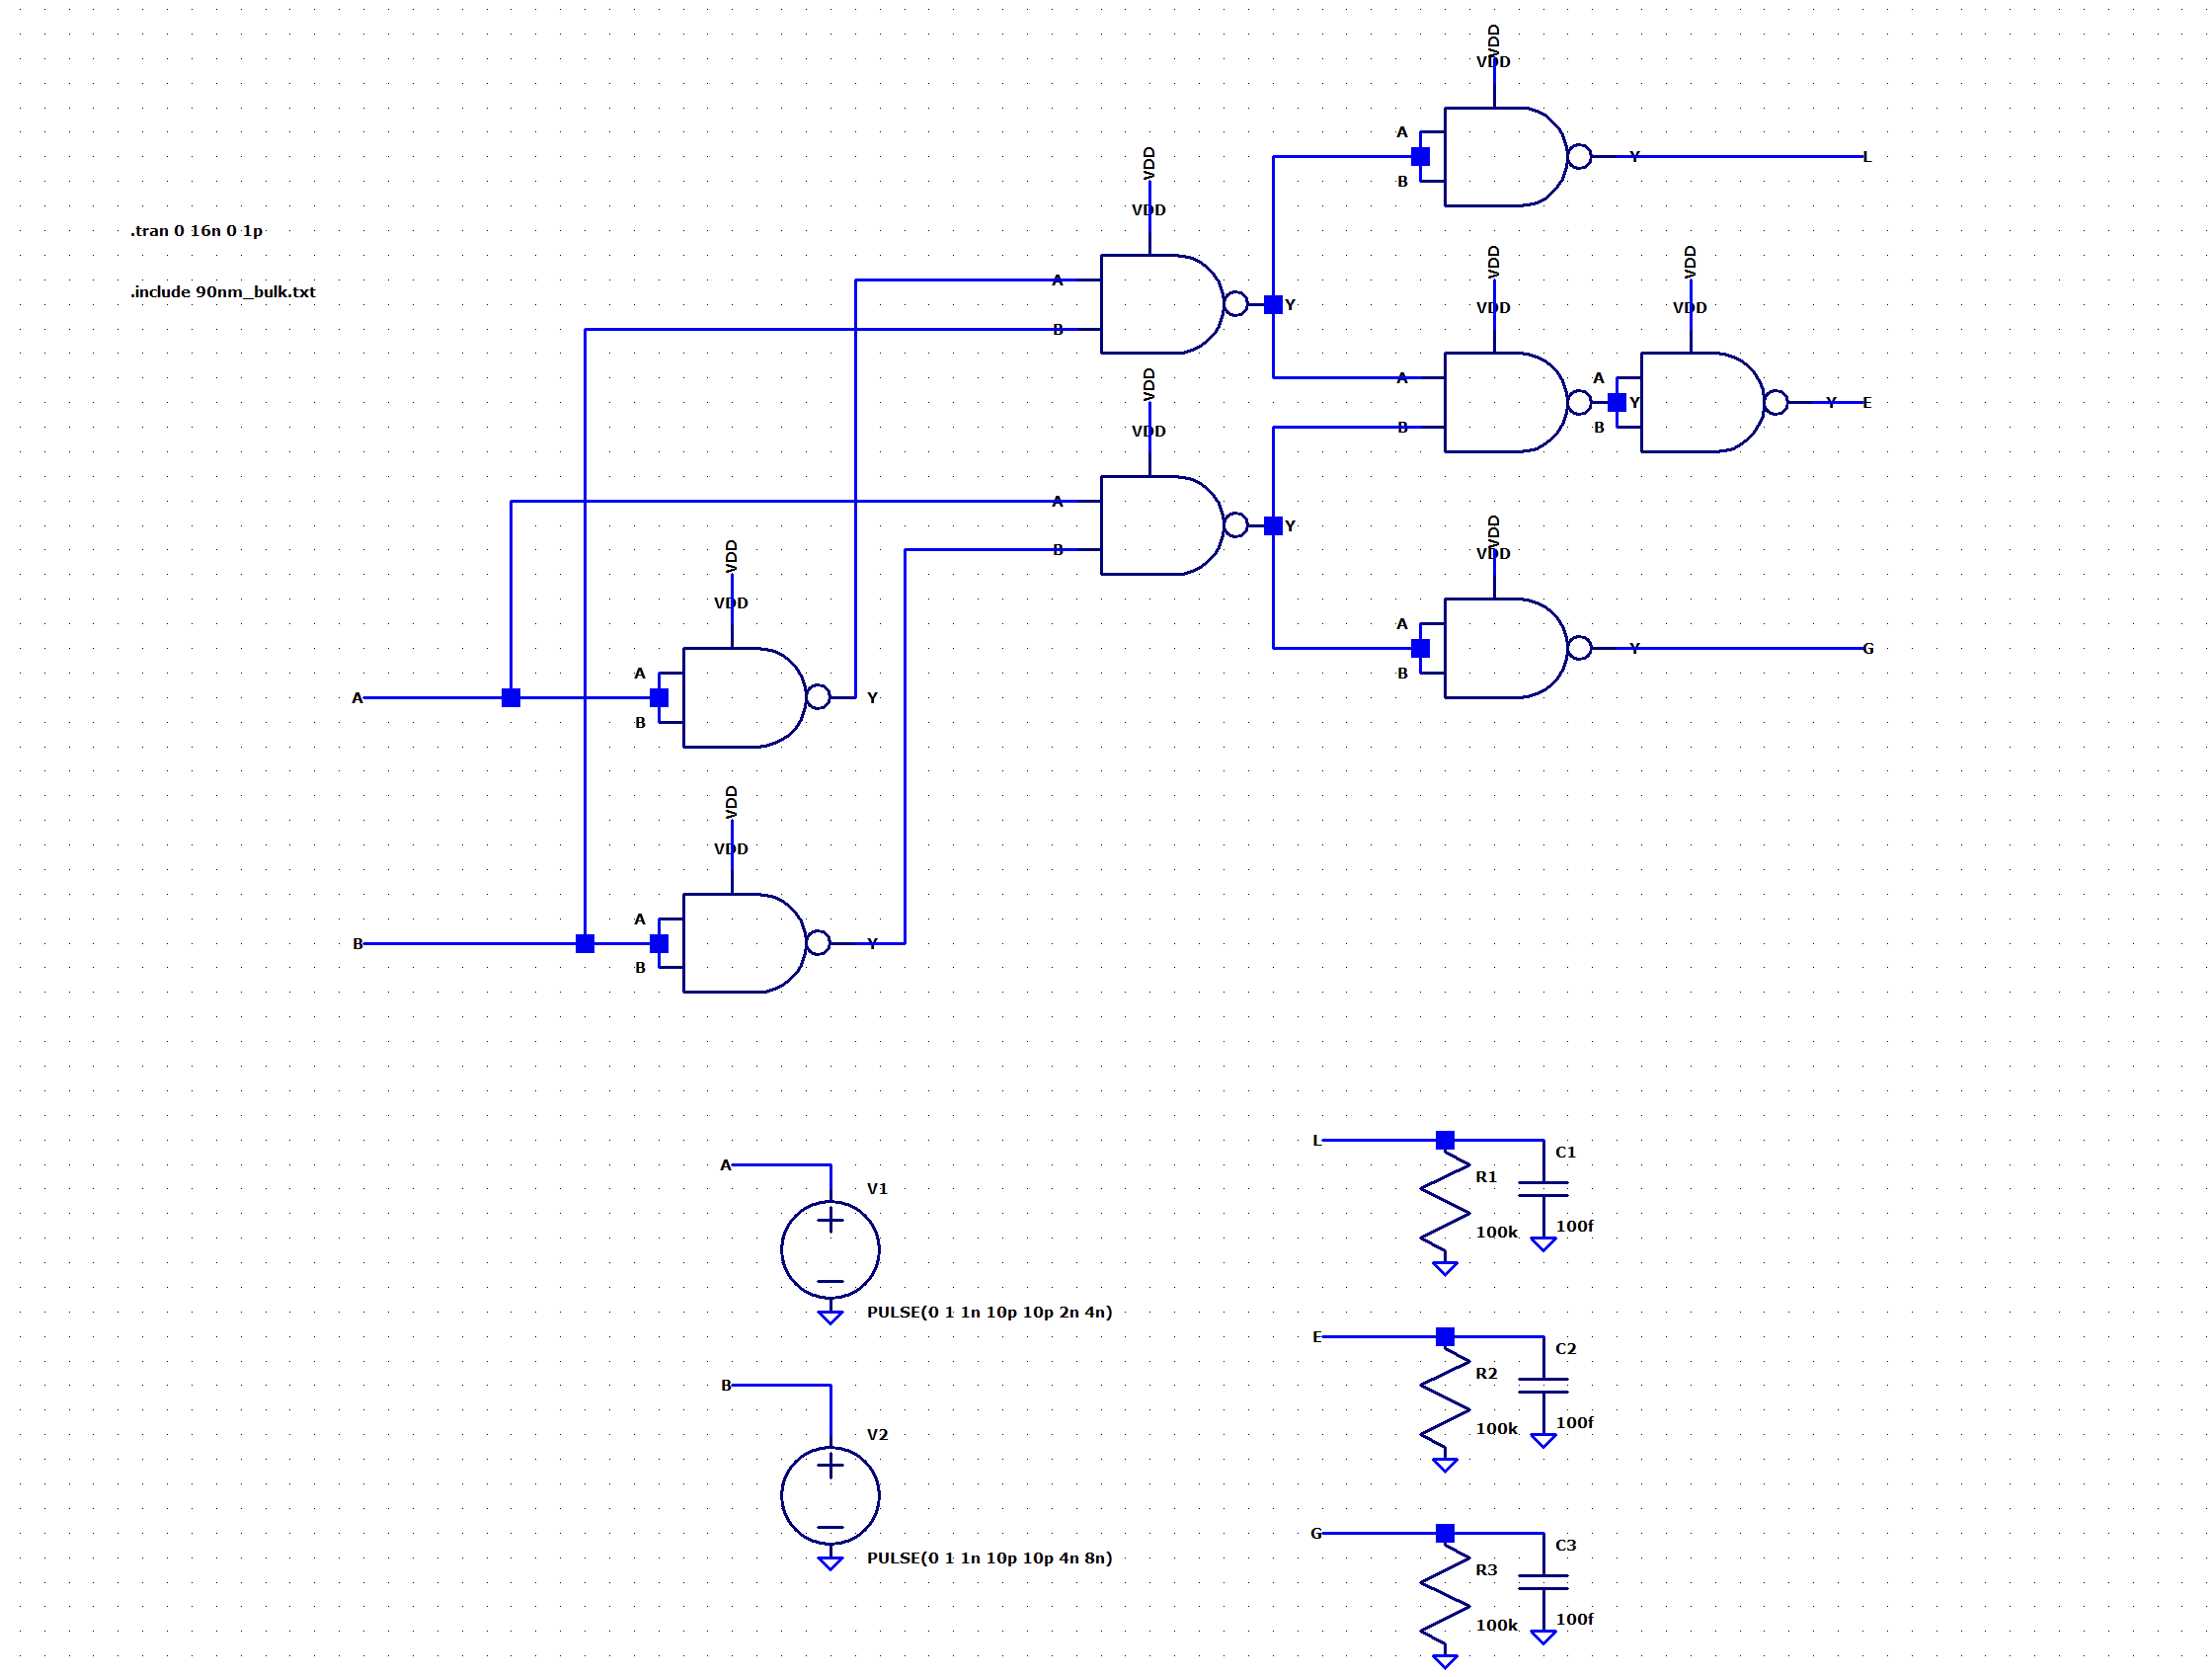
\includegraphics[width=\textwidth]{image/full-comparator1.png}
    \caption{Схема полного компаратора с двумя одноразрядными входами}
\end{figure}
\begin{figure}[H]
    \centering
    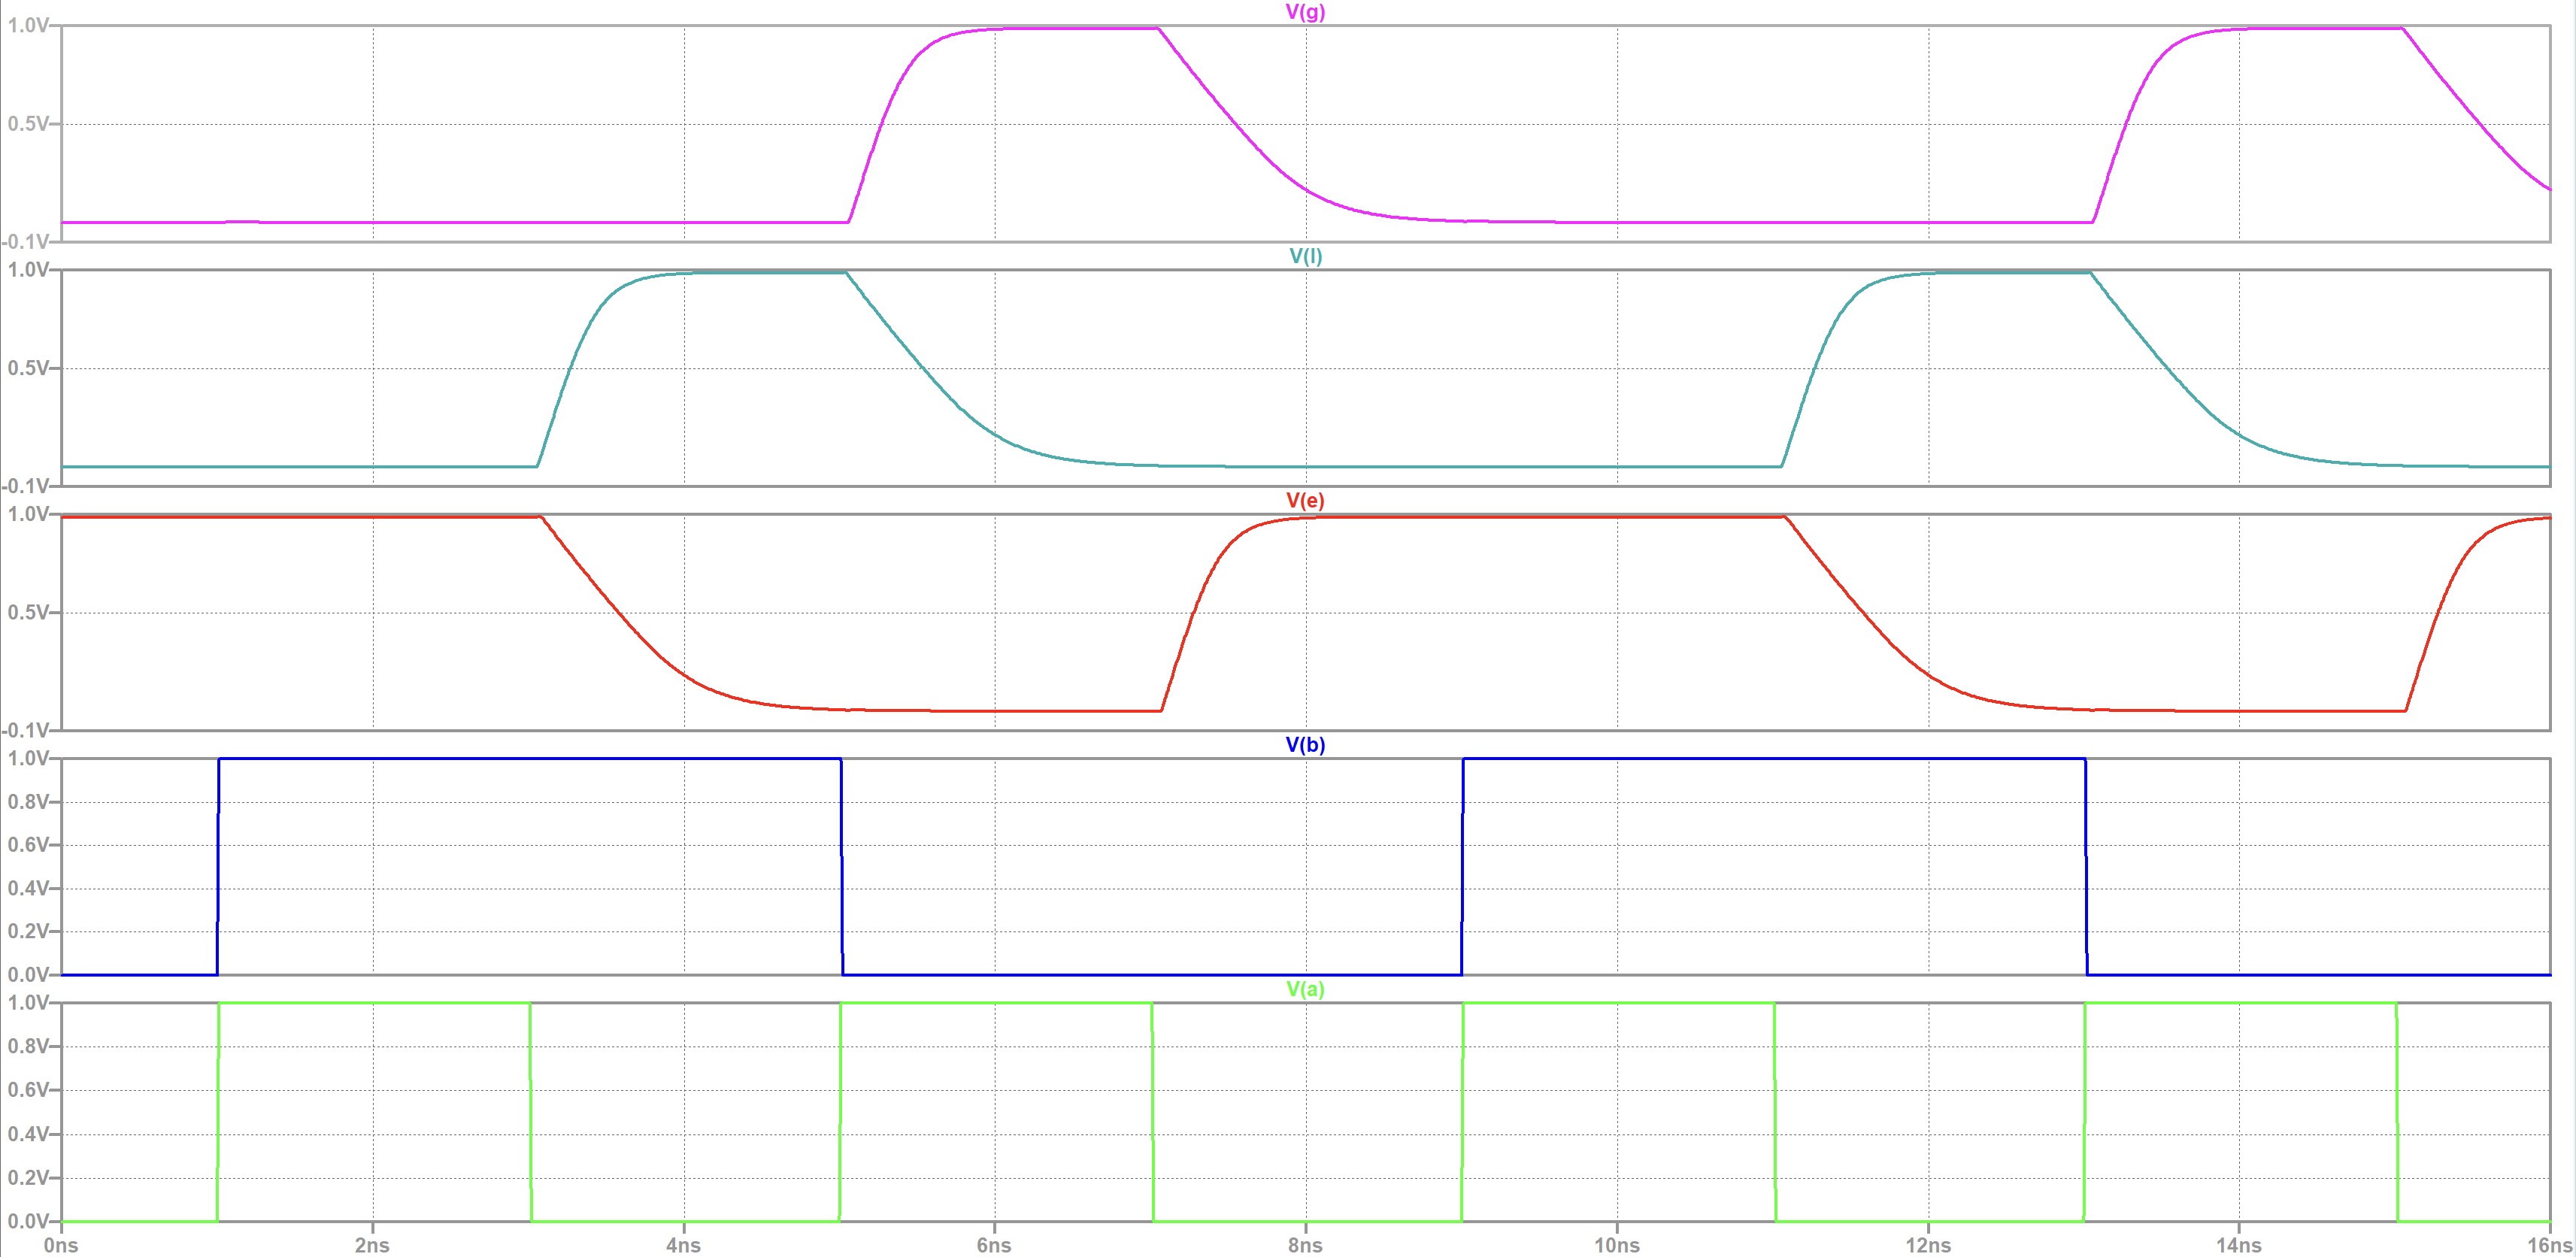
\includegraphics[width=\textwidth]{image/full-comparator1-test.png}
    \caption{Тестирование полного компаратора с двумя одноразрядными входами} 
\end{figure}

Чтобы уменьшить количество обозначений на схеме, сделаем символ полного компаратора с двумя одноразрядными входами
\begin{figure}[H]
    \centering
    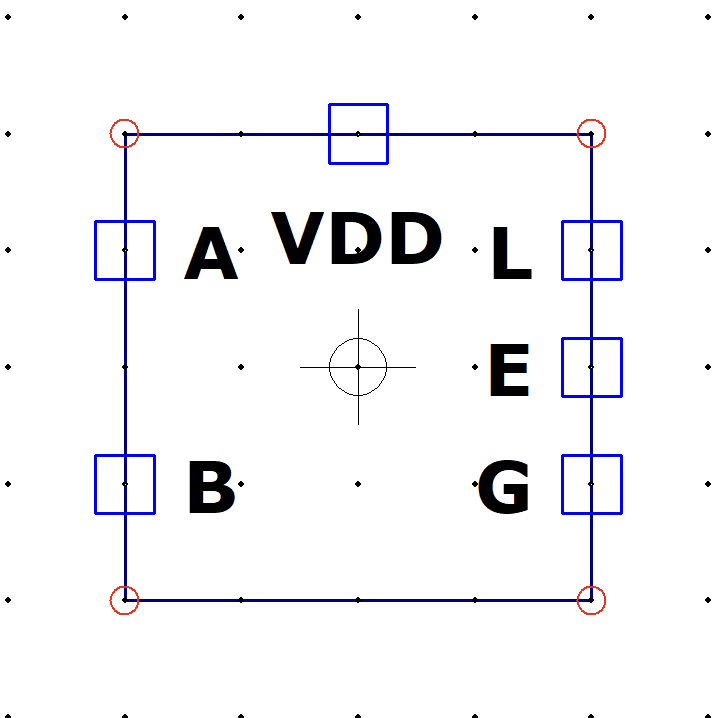
\includegraphics[width=0.3\textwidth]{image/full-comparator1-sym.png}
    \caption{Символ полного компаратора с двумя одноразрядными входами}
\end{figure}
Будем делать последовательный компаратор, поэтому добавим входы наращивания разрядности.
$$A\wedge B = (A \mid B) \mid (A \mid B)$$
$$A \vee B = (A \mid A) \mid (B \mid B)$$
\begin{figure}[H]
    \centering
    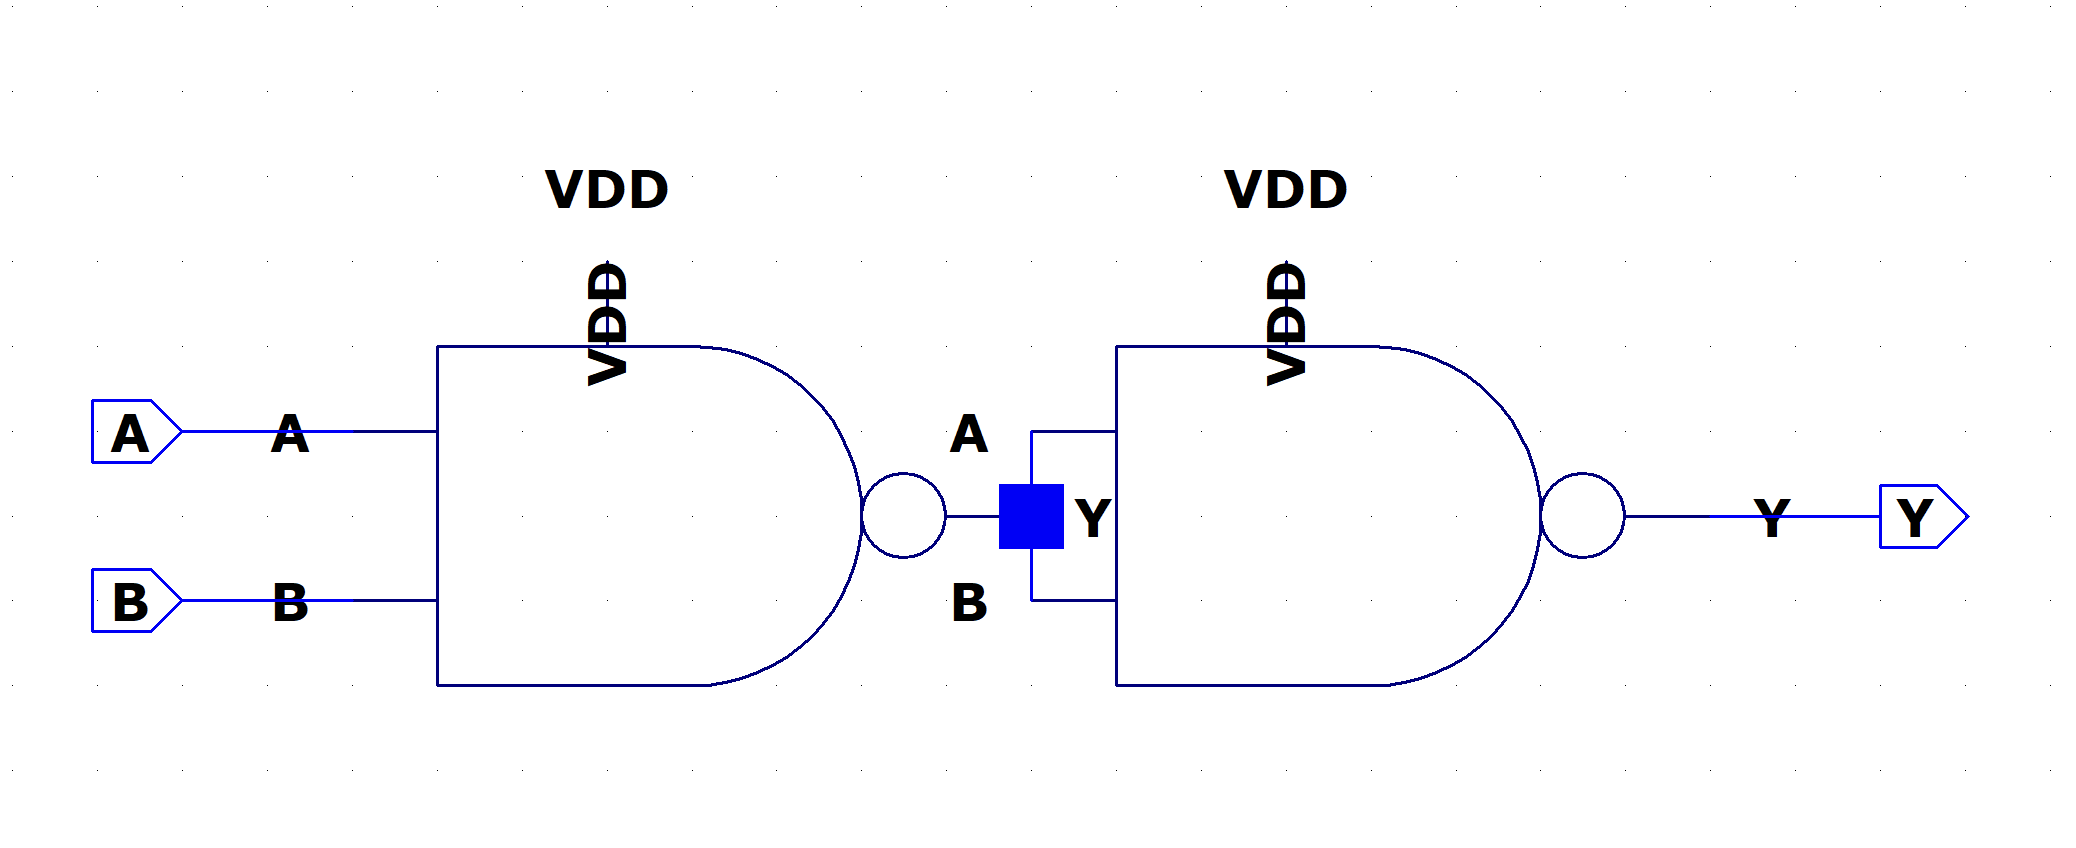
\includegraphics[width=0.5\textwidth]{image/and.png}
    \caption{Схема and}
\end{figure}
\begin{figure}[H]
    \centering
    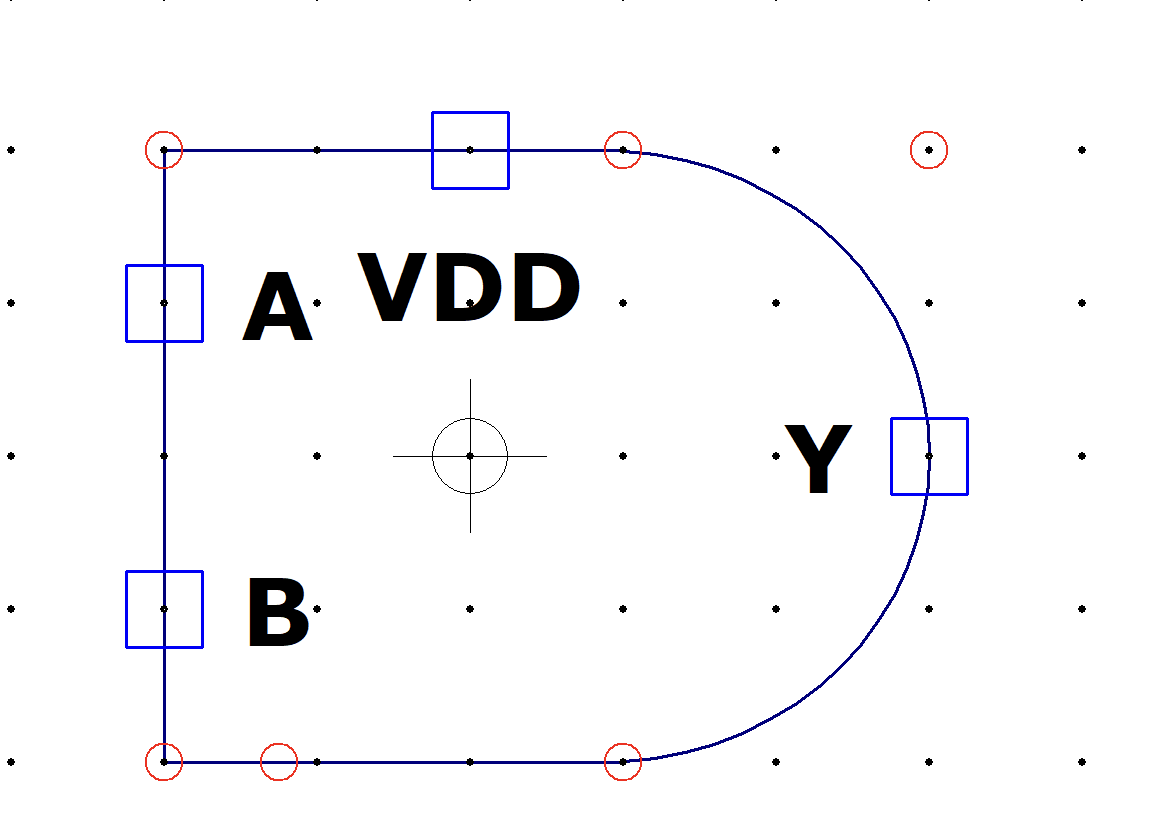
\includegraphics[width=0.2\textwidth]{image/and-sym.png}
    \caption{Символ and}
\end{figure}
\begin{figure}[H]
    \centering
    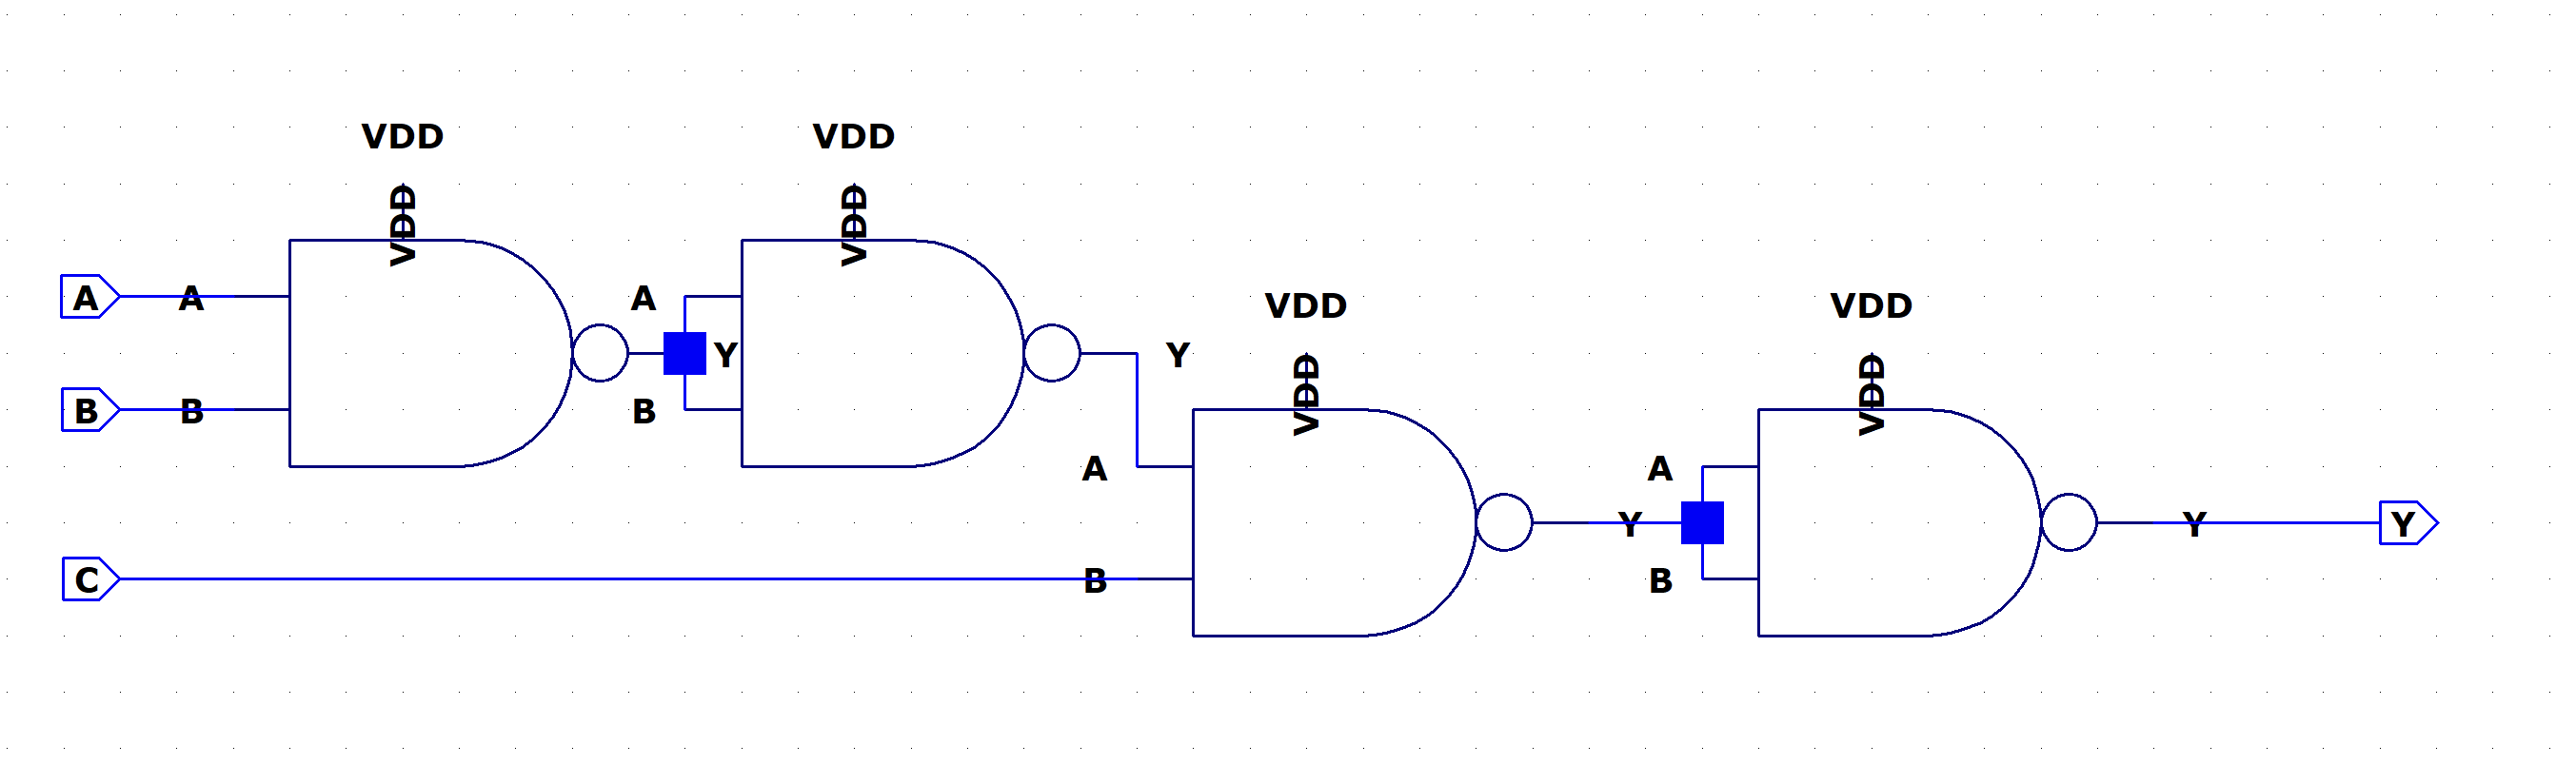
\includegraphics[width=0.5\textwidth]{image/and3.png}
    \caption{Схема and3}
\end{figure}
\begin{figure}[H]
    \centering
    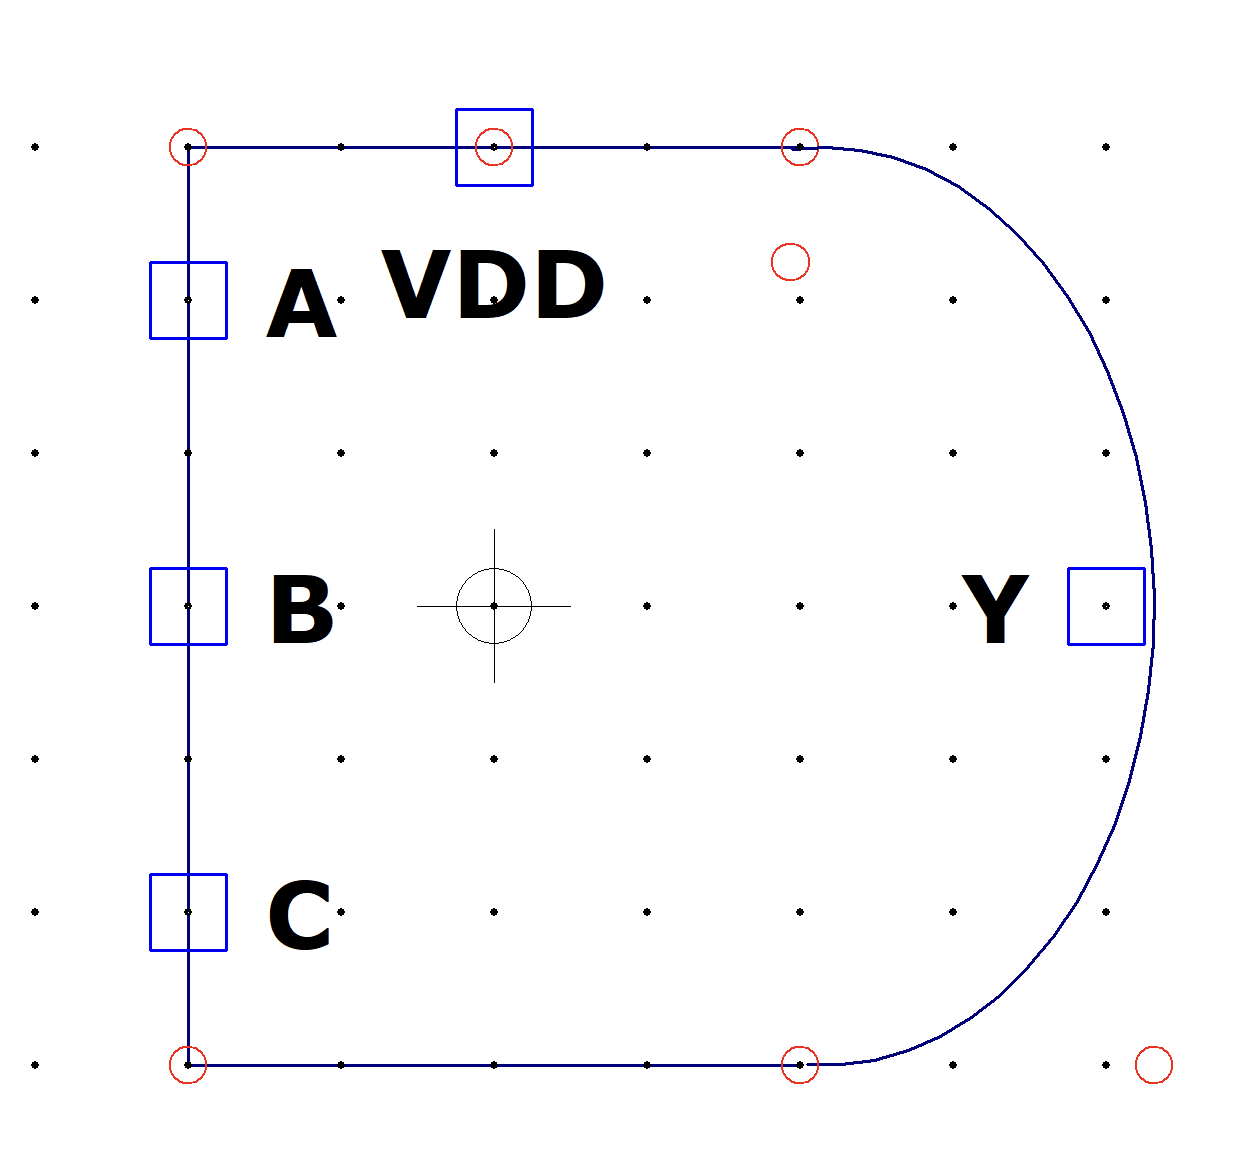
\includegraphics[width=0.2\textwidth]{image/and3-sym.png}
    \caption{Символ and3}
\end{figure}
\begin{figure}[H]
    \centering
    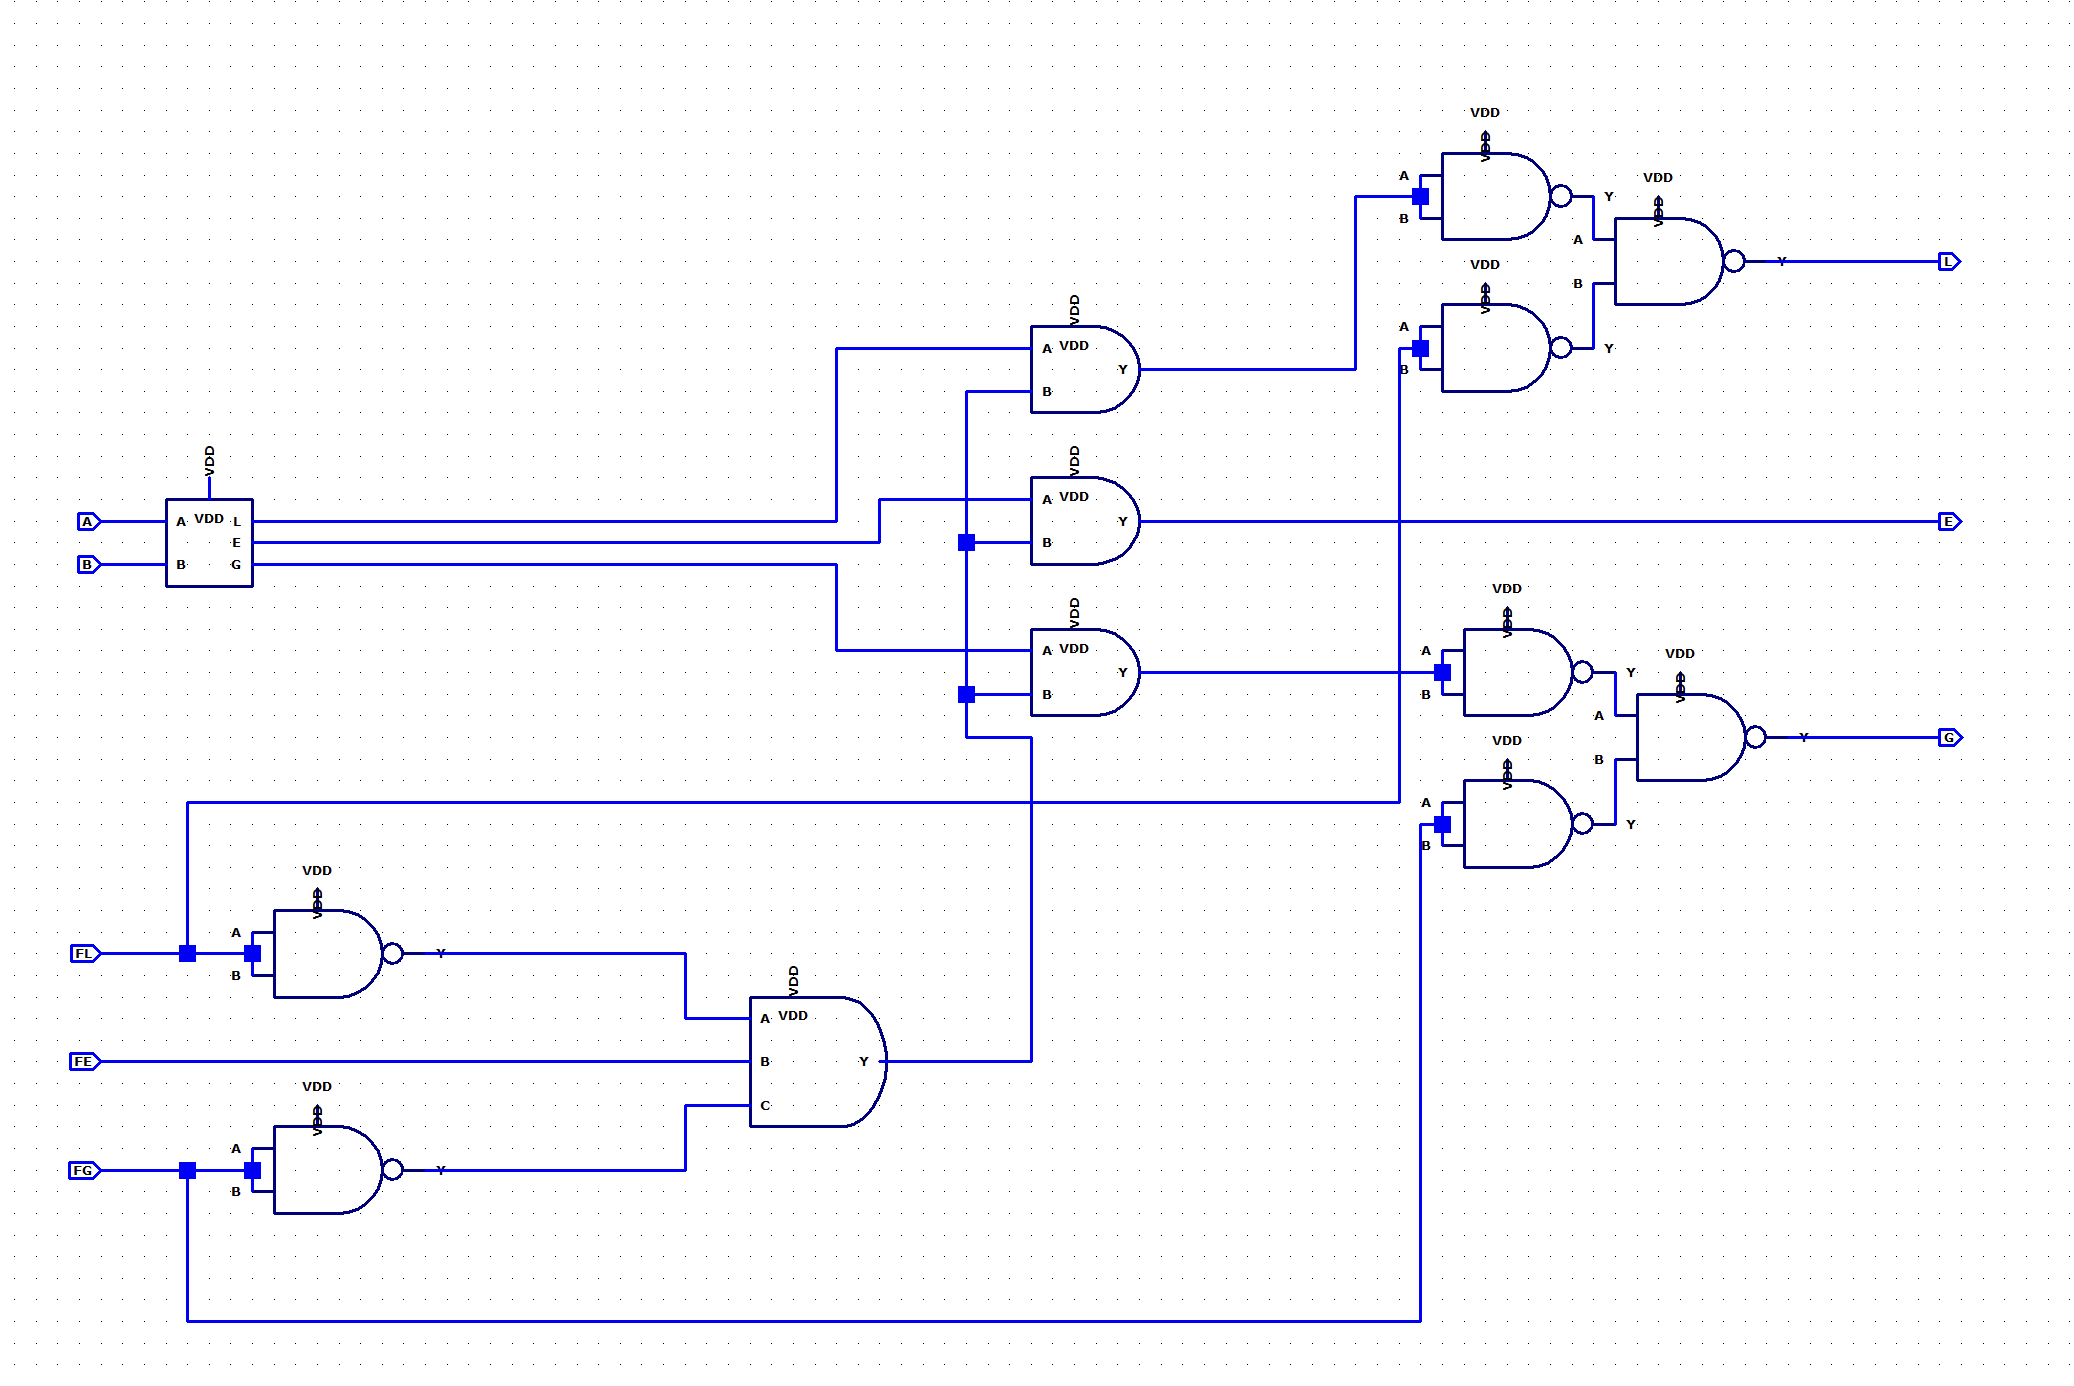
\includegraphics[width=\textwidth]{image/full-comparator-seq.png}
    \caption{Схема полного компаратора с двумя одноразрядными входами и входами наращивания разрядности}
\end{figure}
Чтобы не пугать людей, сделаем ещё символ для полного компаратора с двумя одноразрядными входами и входами наращивания разрядности:
\begin{figure}[H]
    \centering
    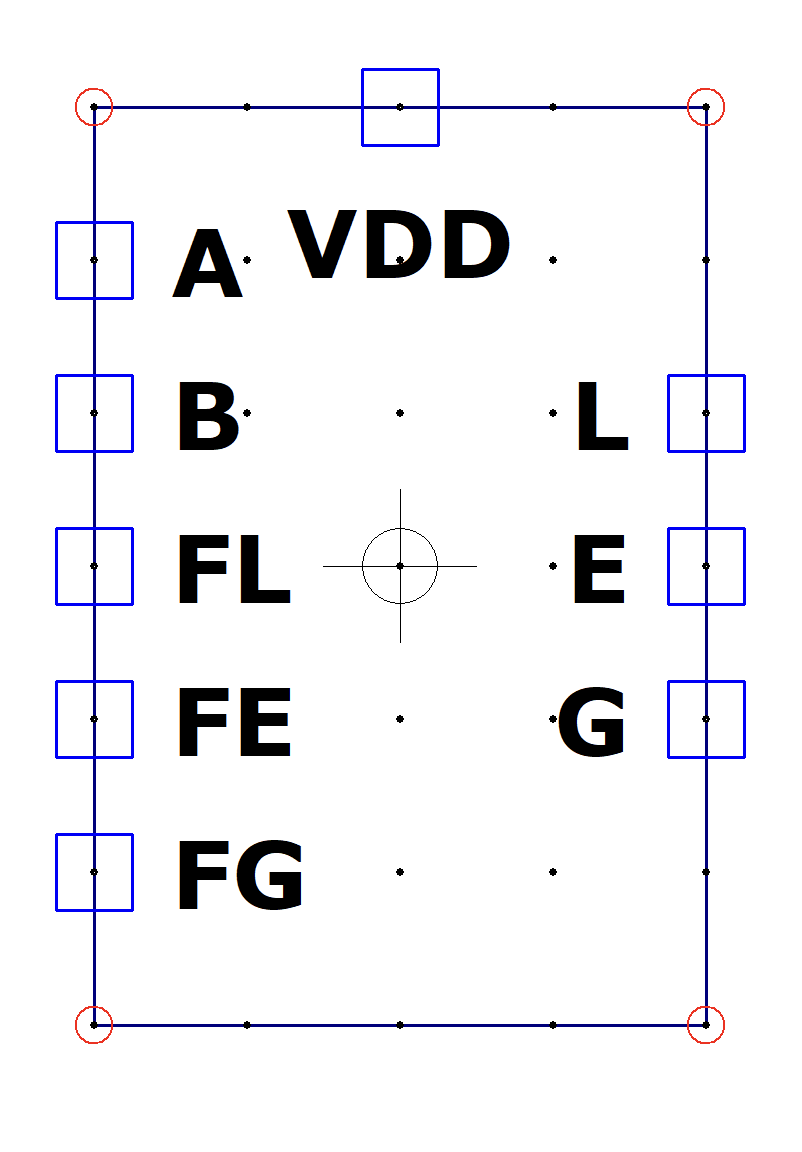
\includegraphics[width=0.3\textwidth]{image/full-comparator-seq-sym.png}
    \caption{Символ полного компаратора с двумя одноразрядными входами и входами наращивания разрядности}
\end{figure}
Подключим компараторы в последовательную цепочку, чтобы получить полный четырехразрядный компаратор.
Насладимся красатой получившейся схемы, не забывая про тестирование на каждом из этапов.
\begin{figure}[H]
    \centering
    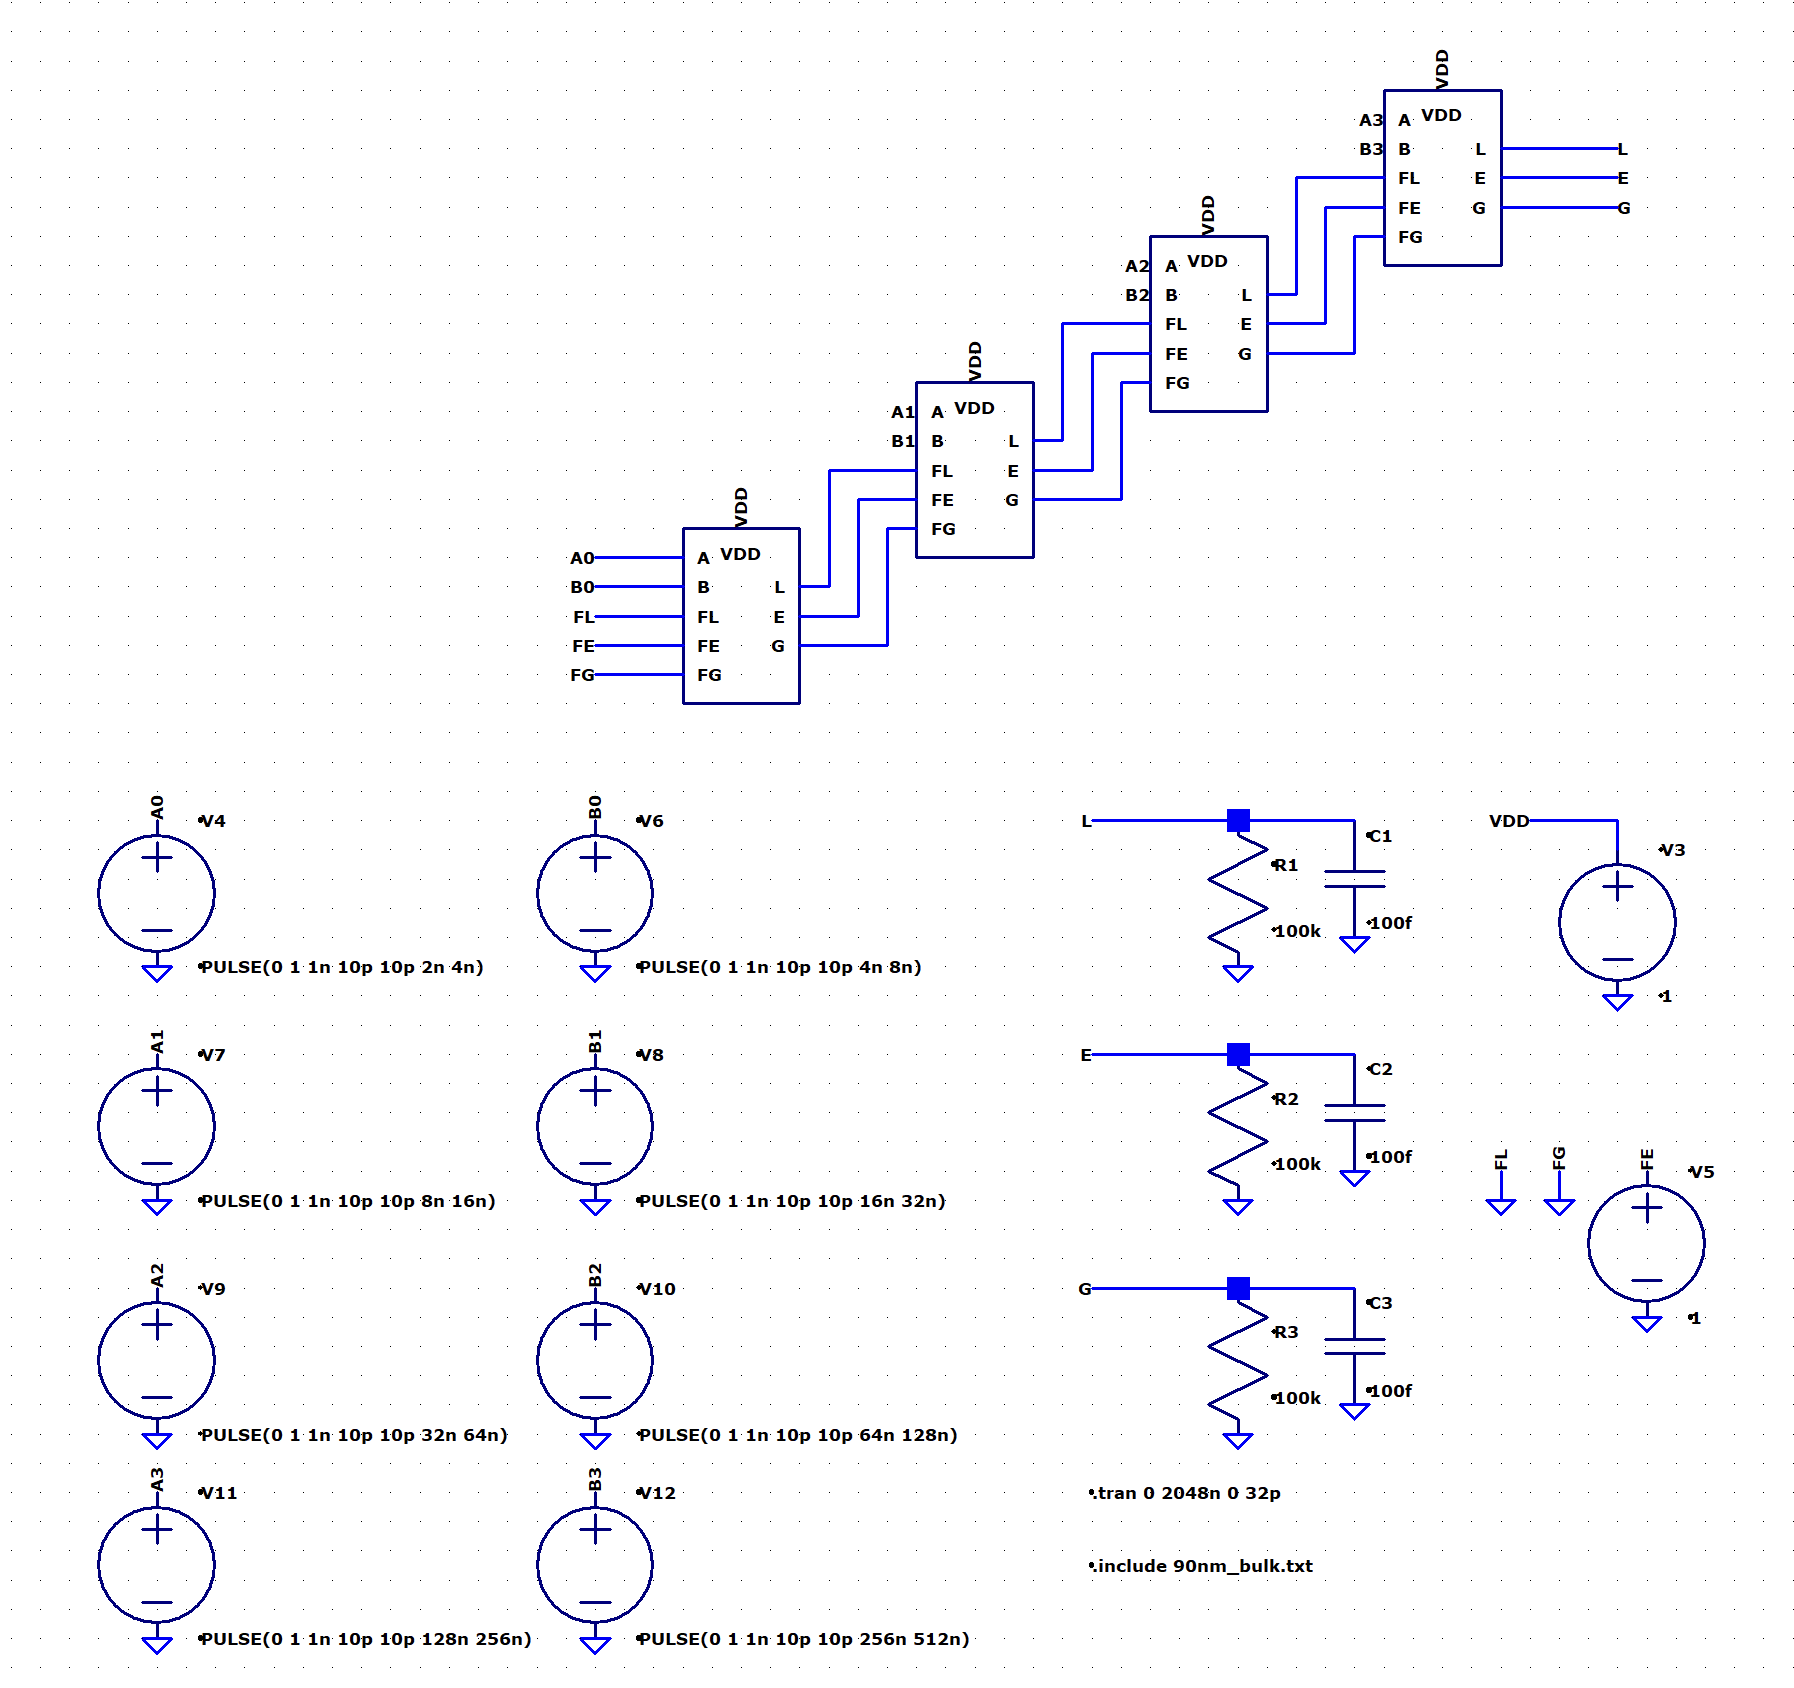
\includegraphics[width=\textwidth]{image/full-comparator.png}
    \caption{Схема полного четырехразрядного компаратора}
\end{figure}
\subsection{Создайте символ для построенного БОЭ.}
\begin{figure}[H]
    \centering
    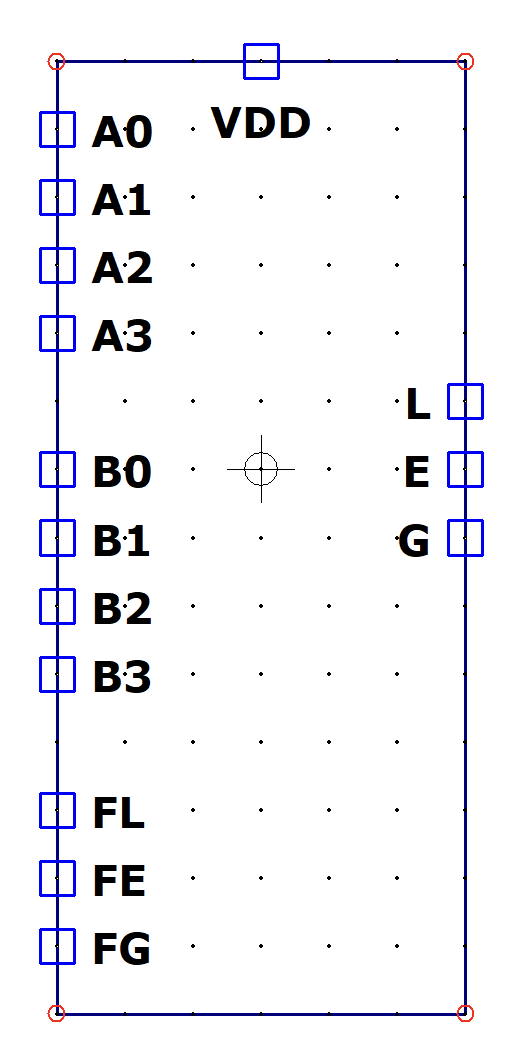
\includegraphics[width=0.3\textwidth]{image/full-comparator-sym.png}
    \caption{Символ полного четырехразрядного компаратора}
\end{figure}
\subsection{Проведите моделирование работы схемы и определите задержку распространения сигнала через БОЭ.}
\begin{figure}[H]
    \centering
    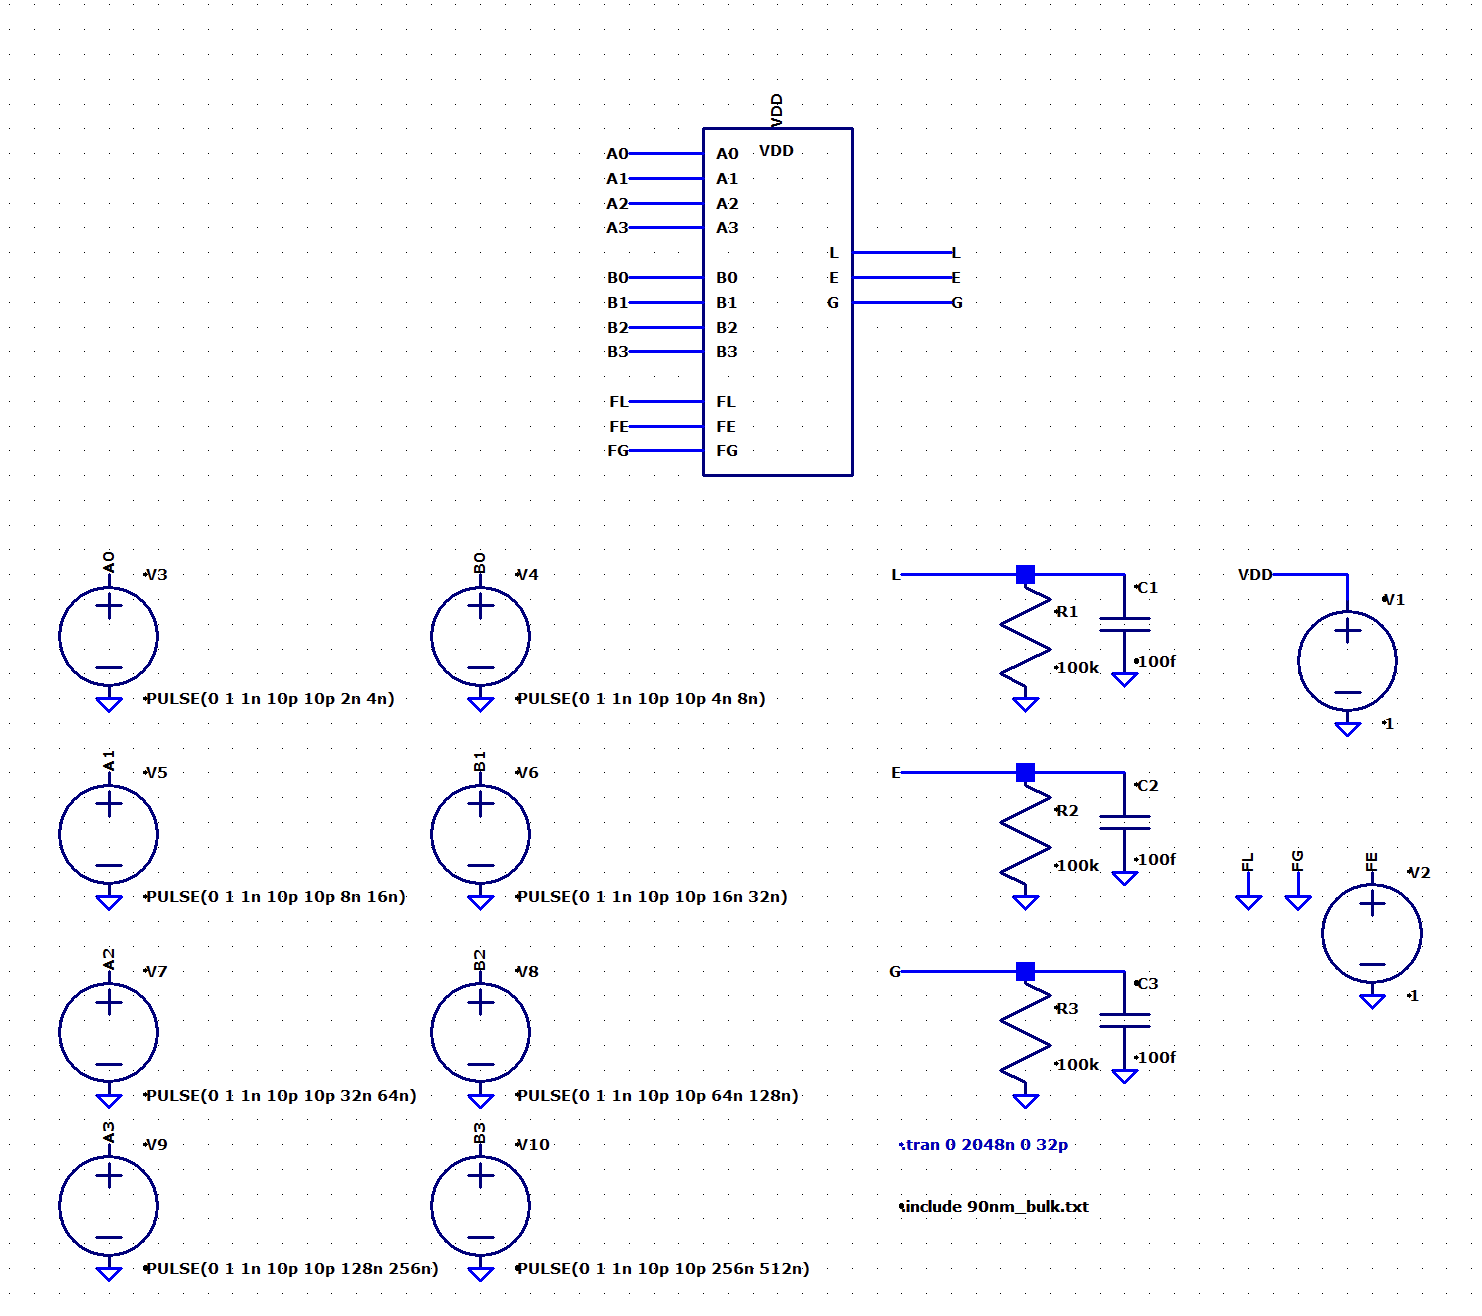
\includegraphics[width=\textwidth]{image/full-comparator-test-env.png}
    \caption{Схема тестирование полного четырехразрядного компаратора}
\end{figure}
\begin{figure}[H]
    \centering
    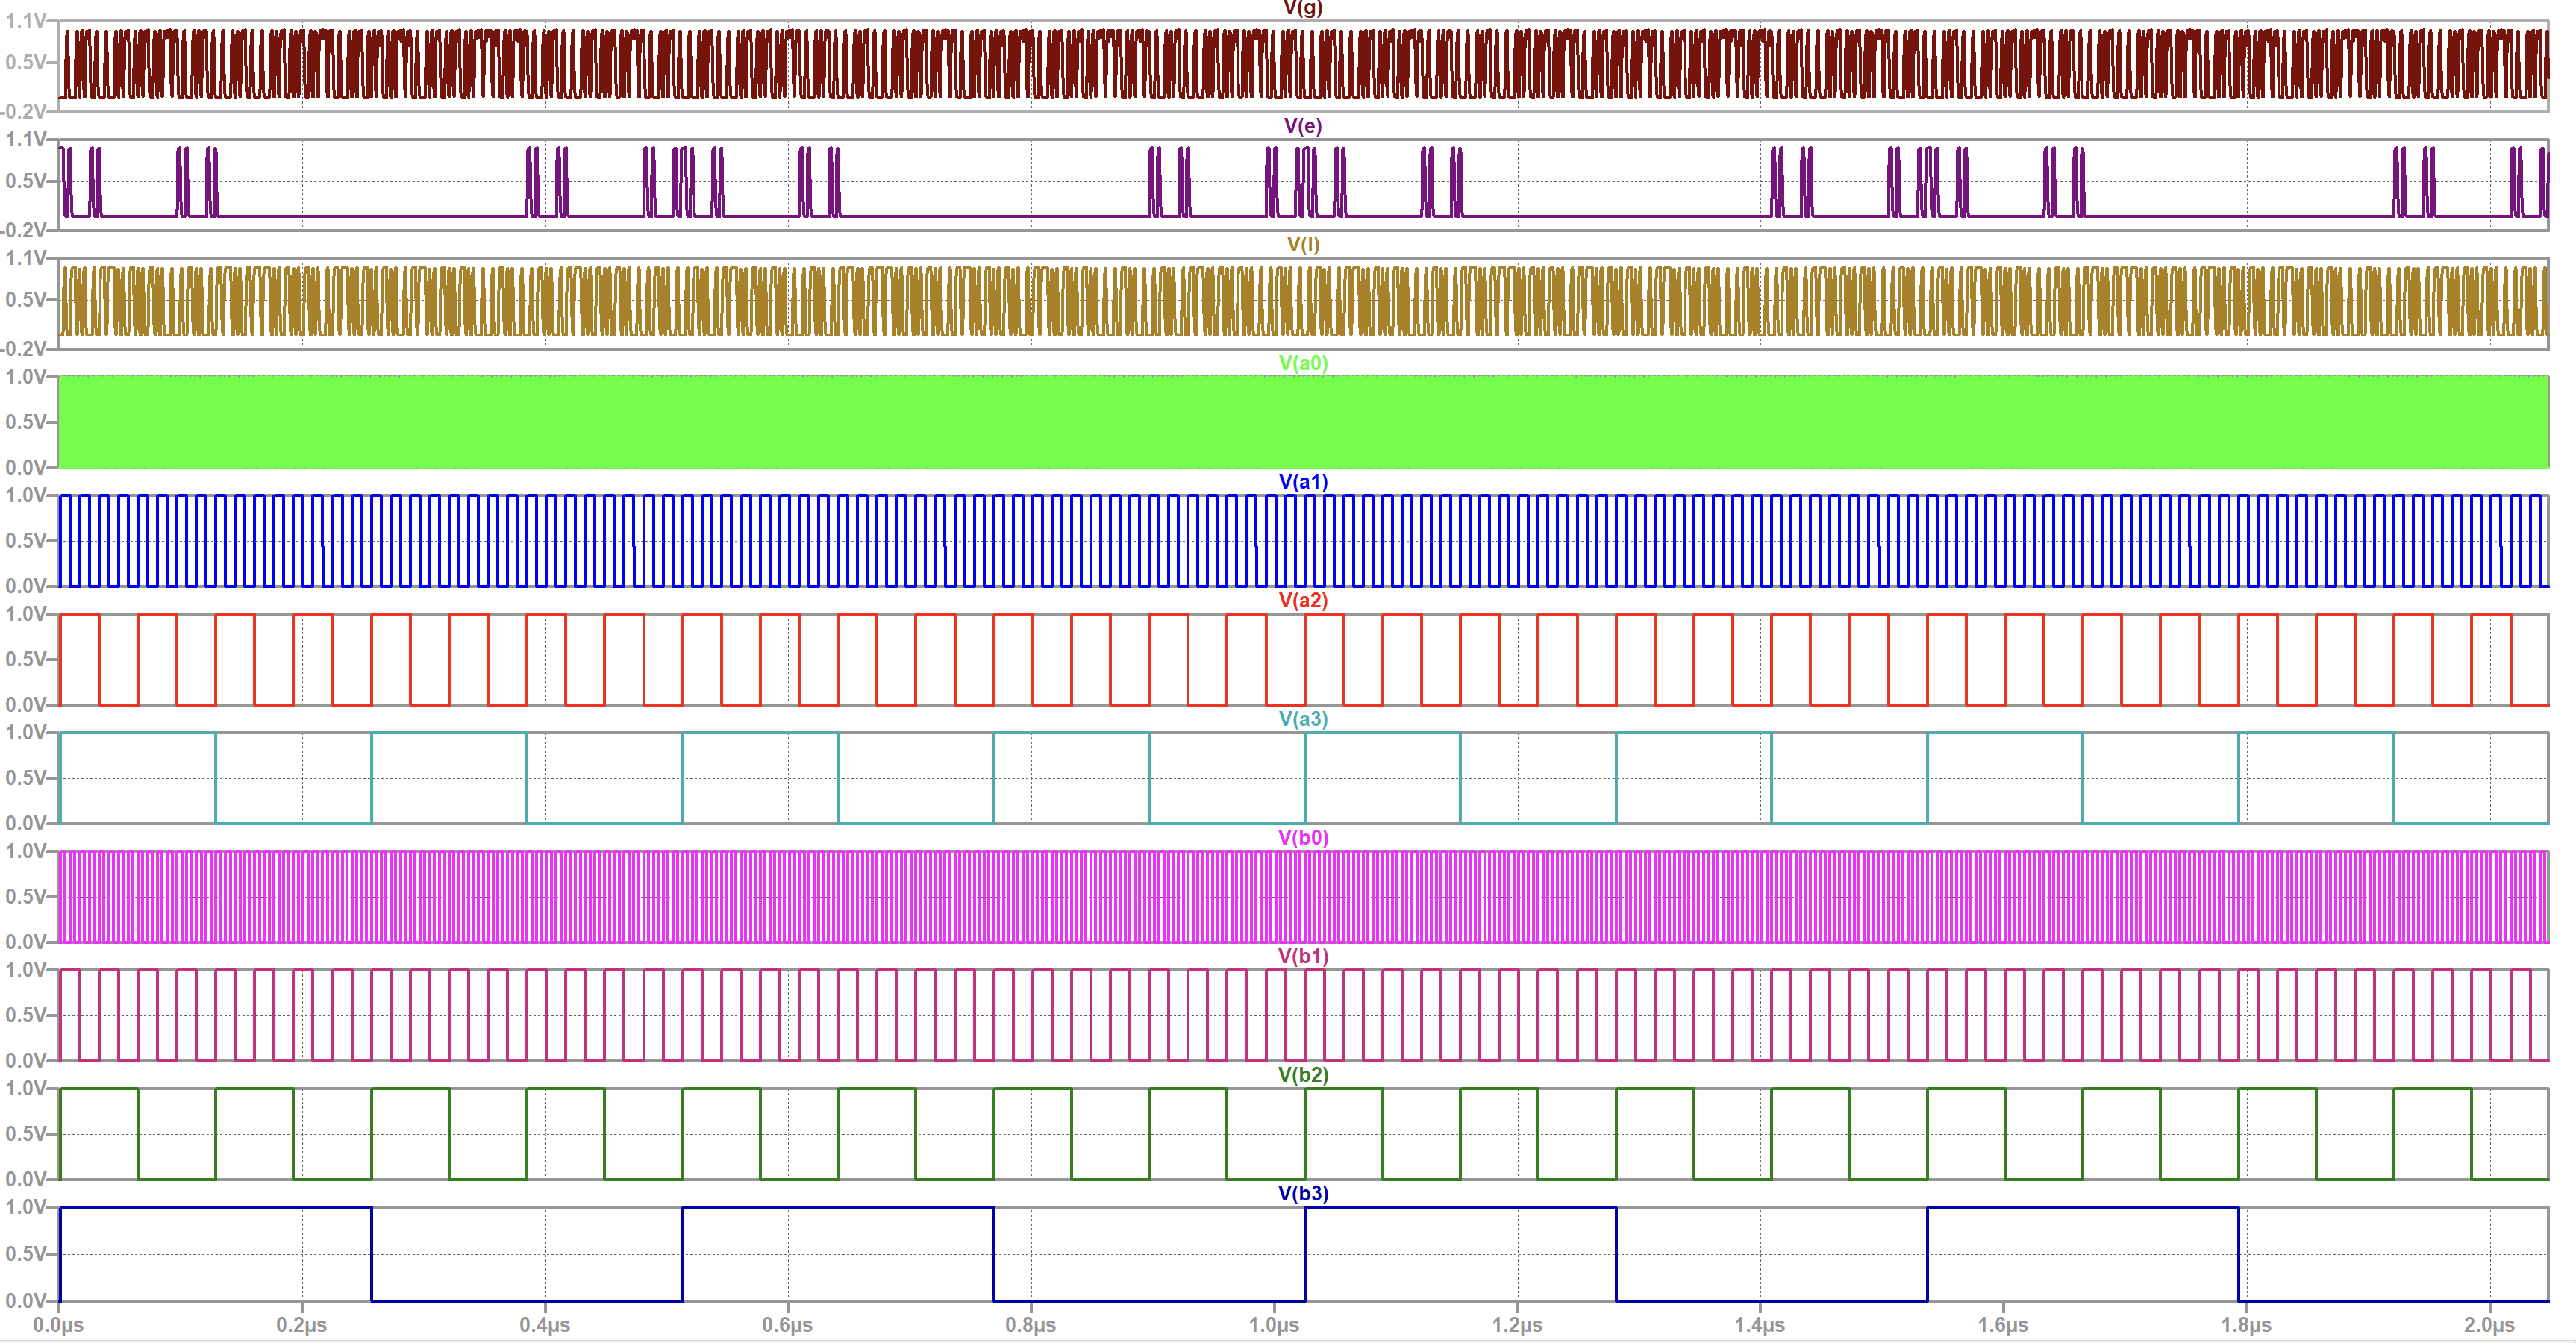
\includegraphics[width=\textwidth]{image/full-comparator-test-all-states.png}
    \caption{Все возможные состояния.}
\end{figure}
\begin{figure}[H]
    \centering
    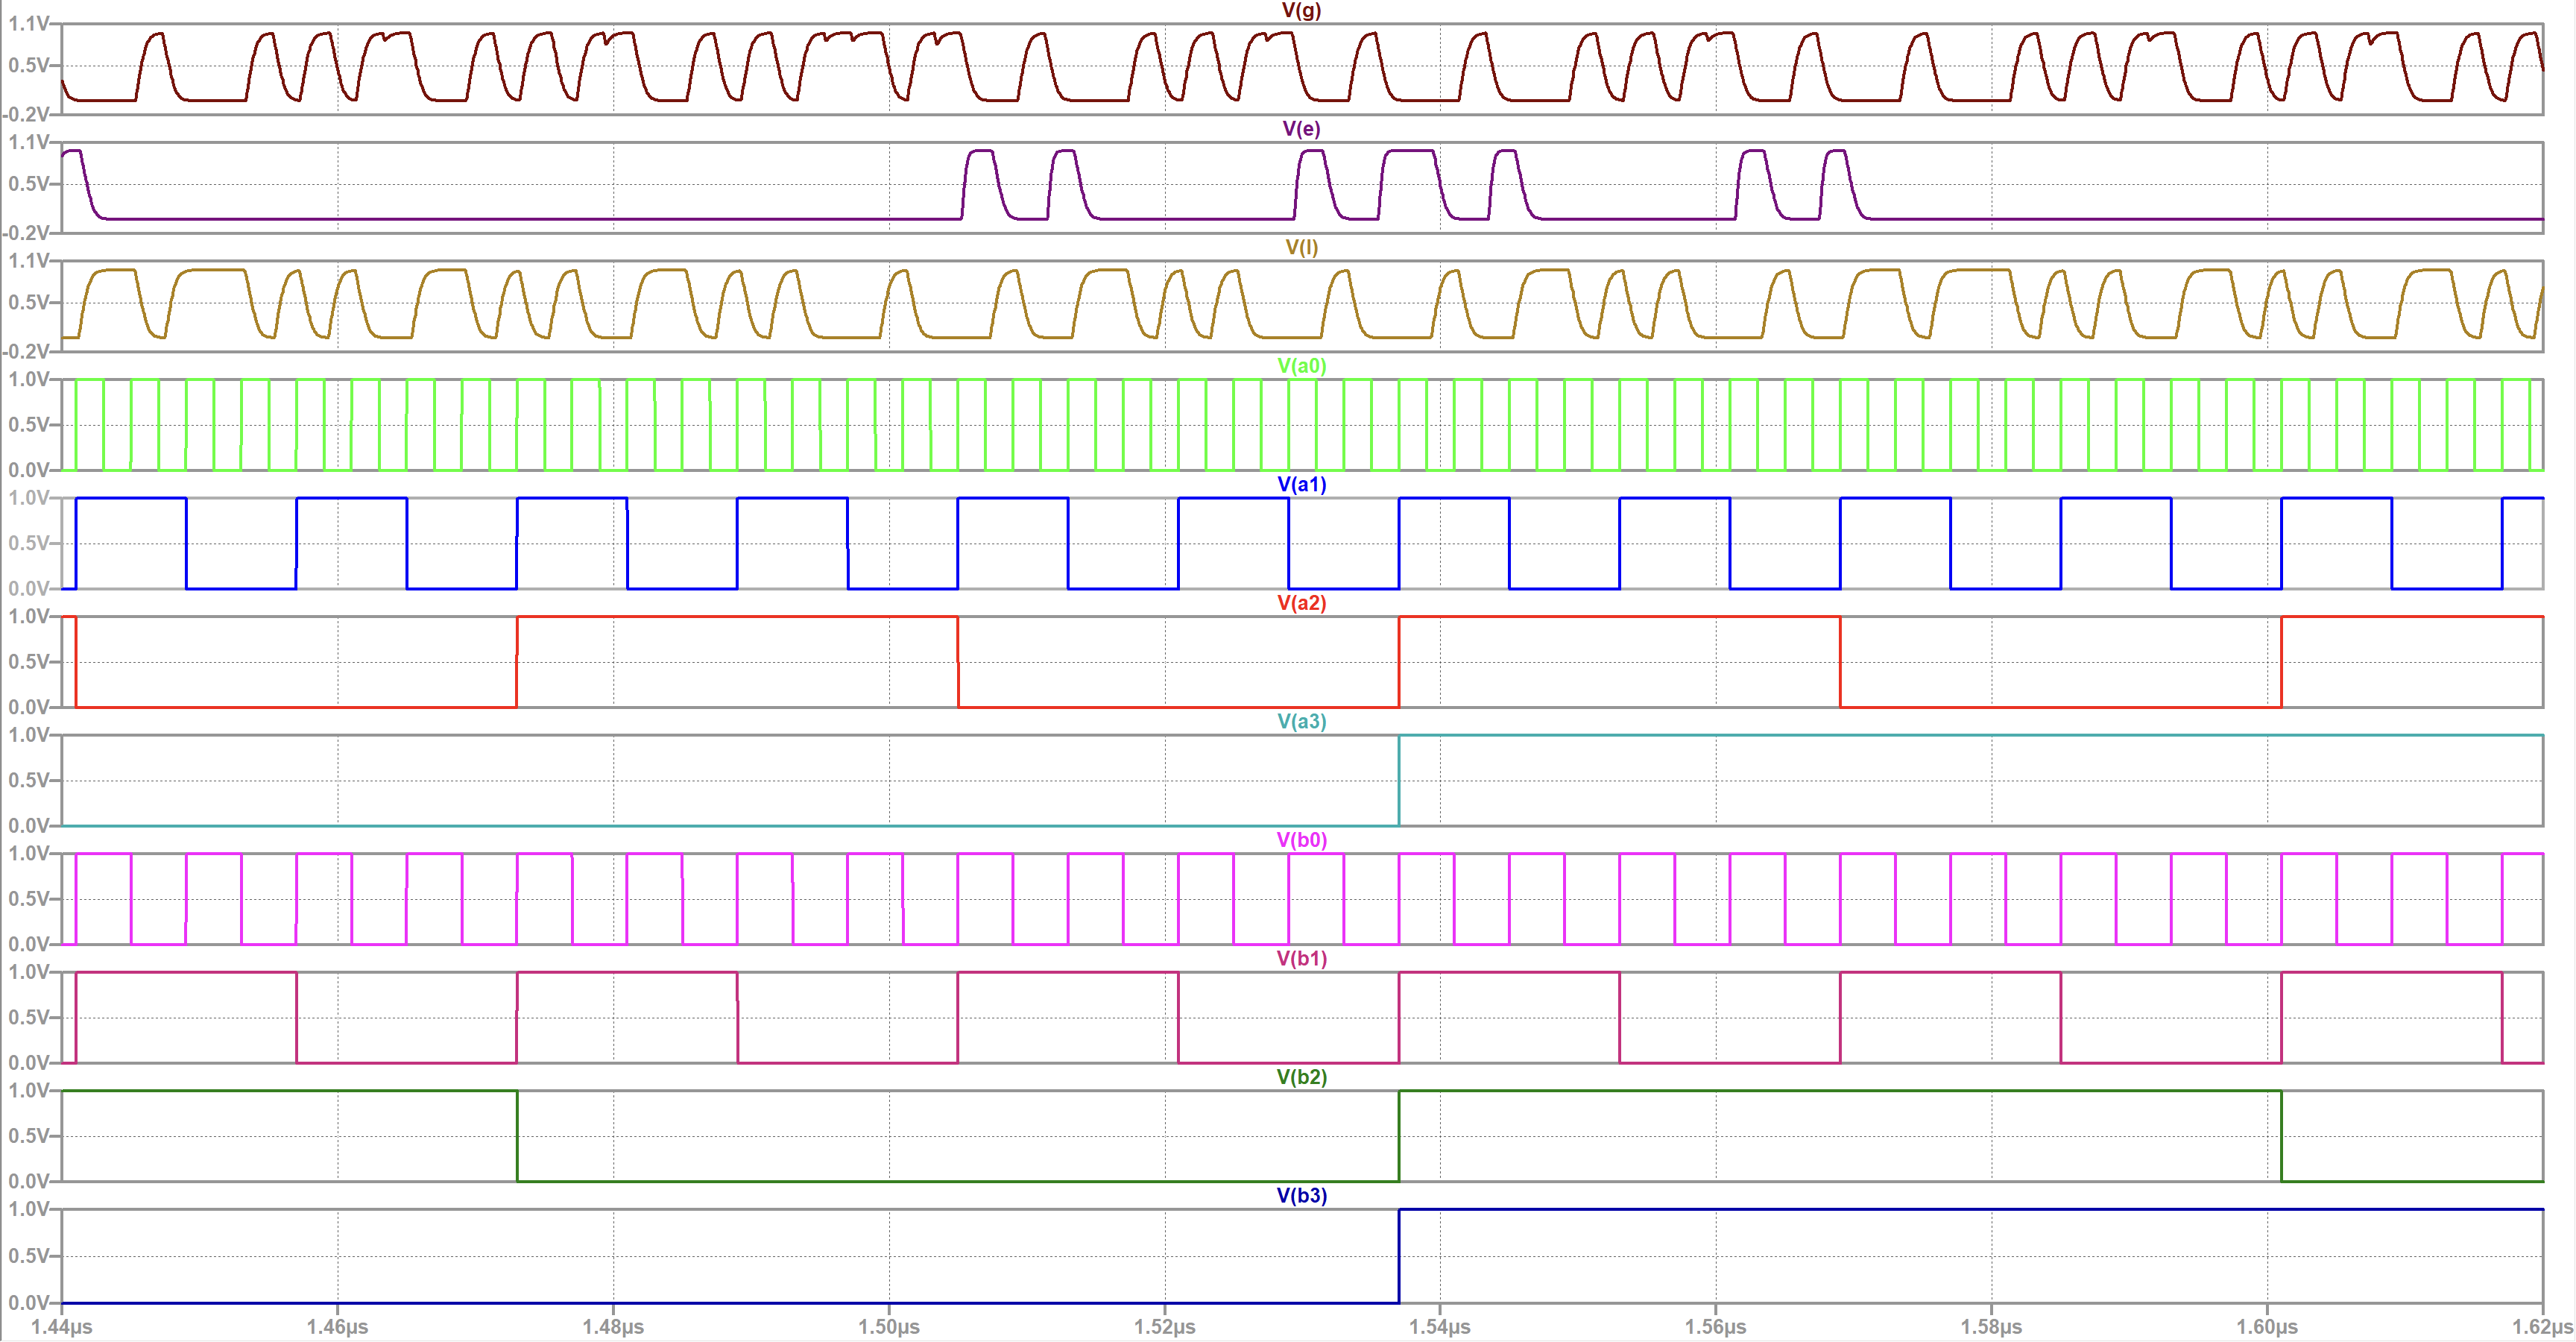
\includegraphics[width=\textwidth]{image/full-comparator-test-zoom.png}
    \caption{Рассмотрим поближе. Видим, что компаратор выдает верные значения}
\end{figure}
\subsection{Результат измерения задержки распространения сигнала через БОЭ}
\begin{figure}[H]
    \centering
    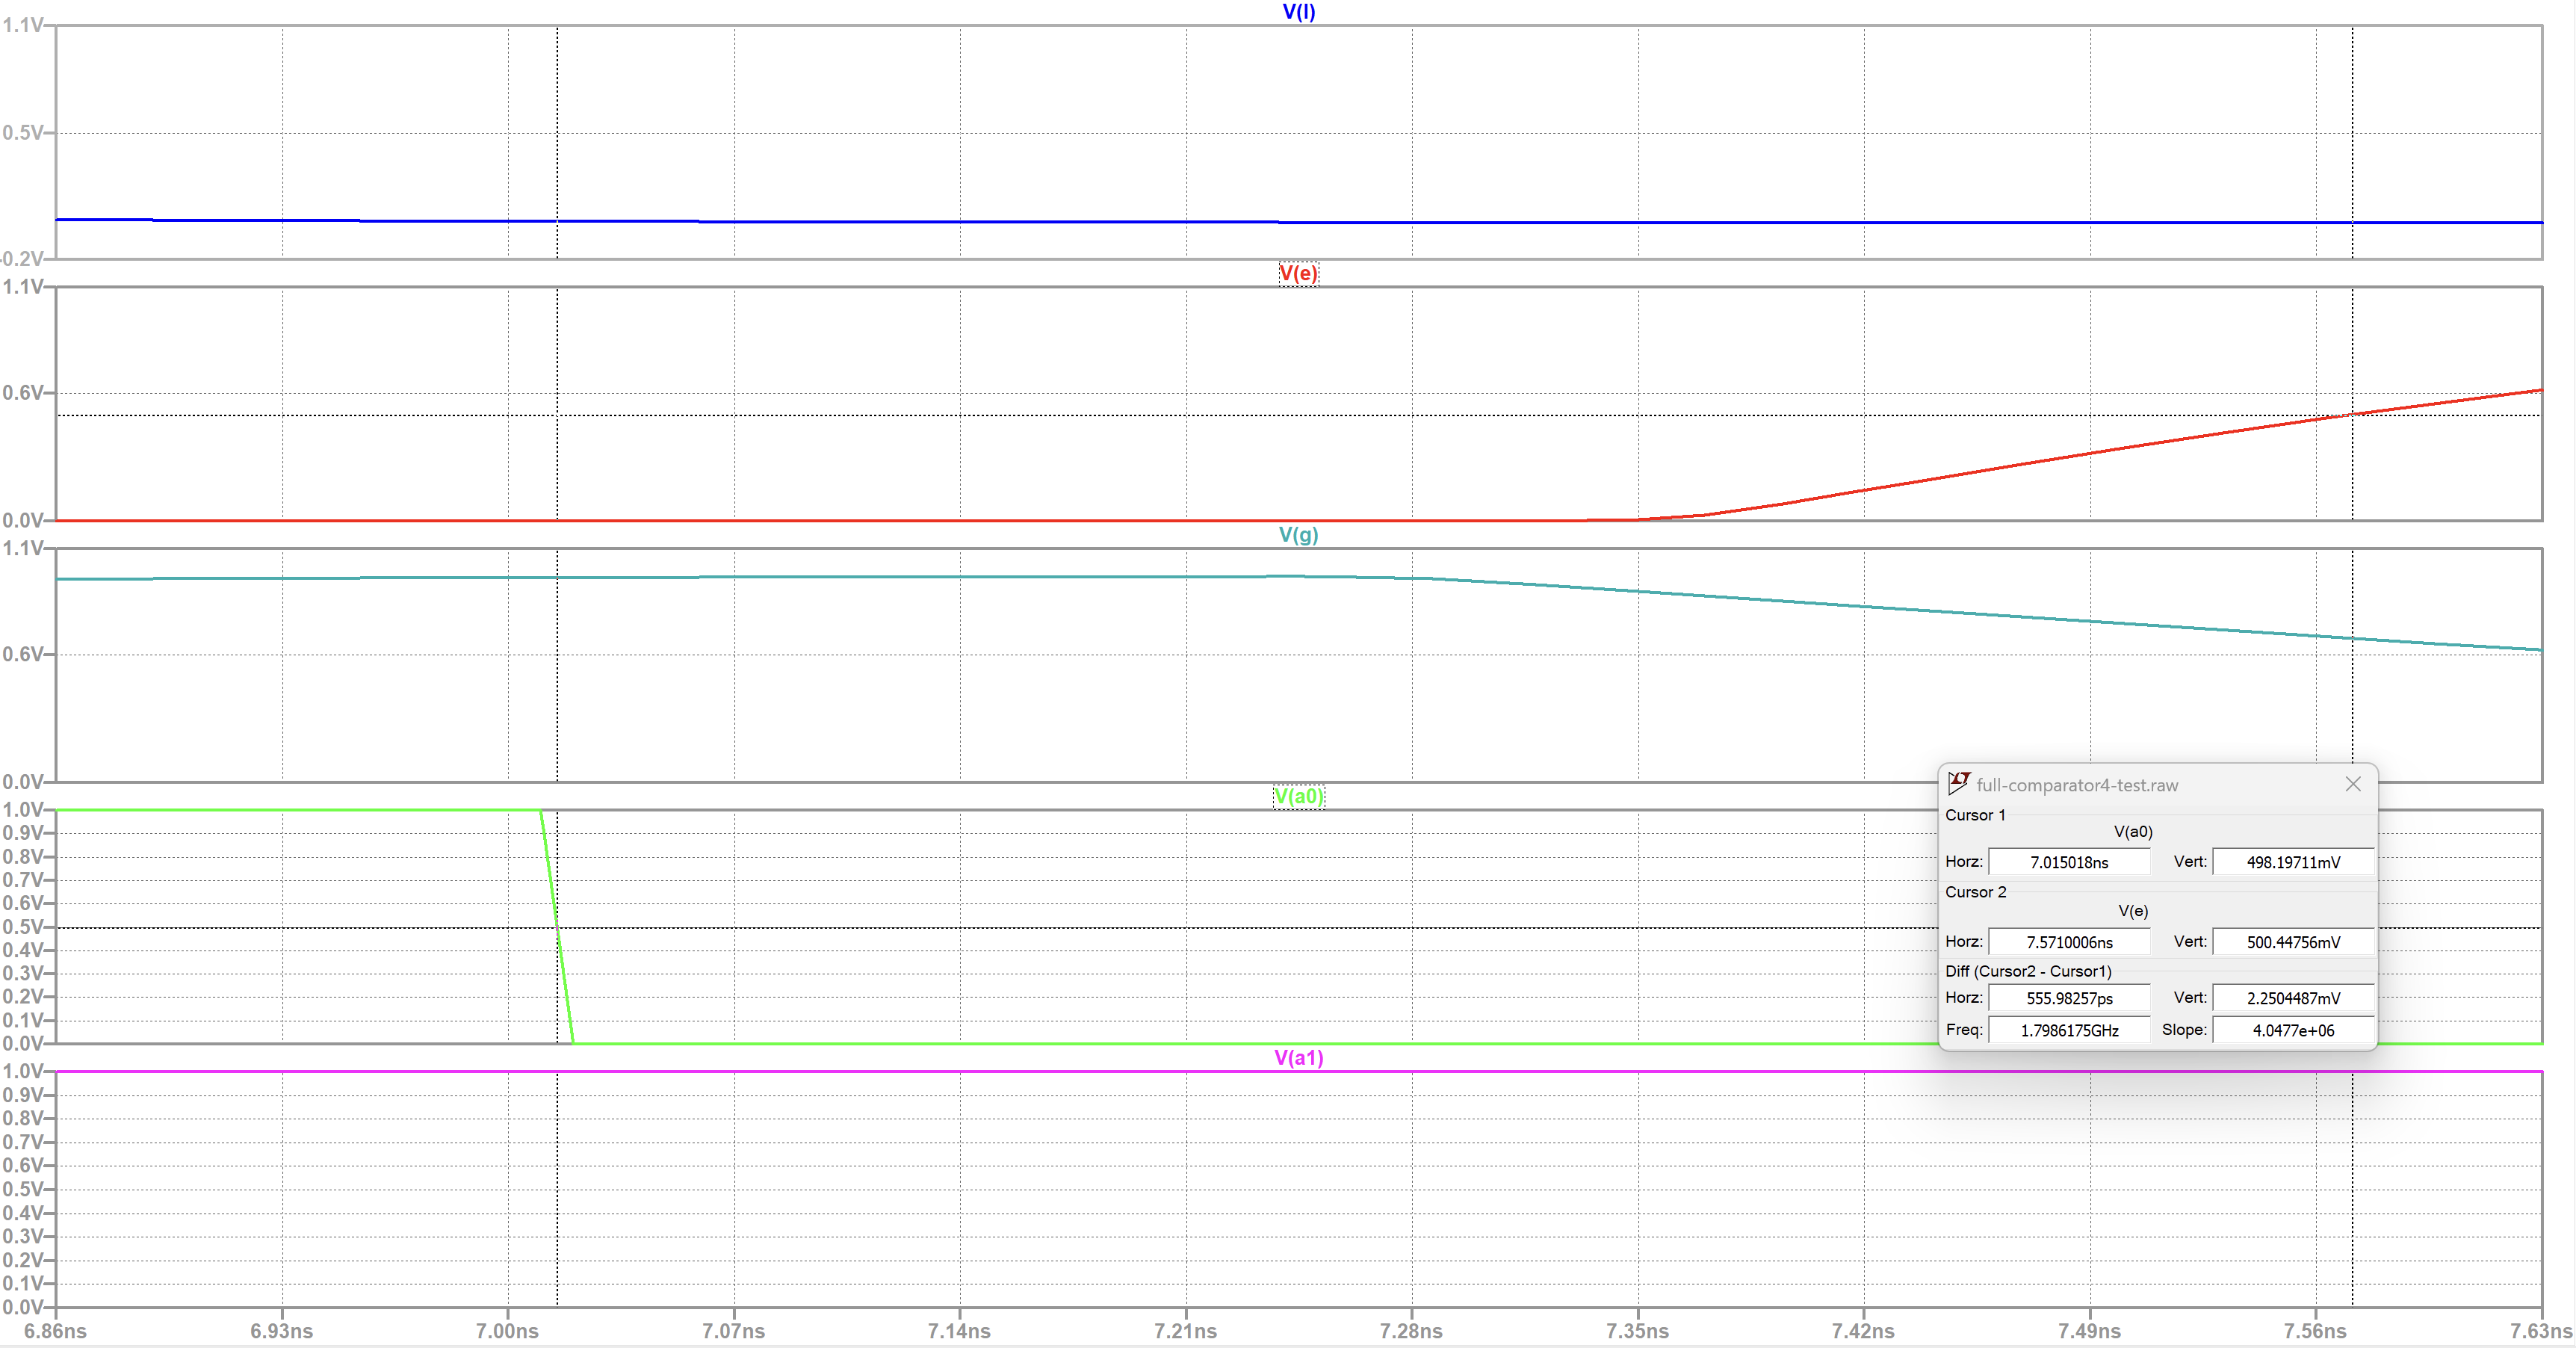
\includegraphics[width=\textwidth]{image/full-comparator-test-eq-01.png}
    \caption{Подсчет задержки распространения сигнала для 0-1 на выходе equal}
\end{figure}

$$t_{\text{pd}} = 7.571 - 7.015 = 0.556 ns$$
\begin{figure}[H]
    \centering
    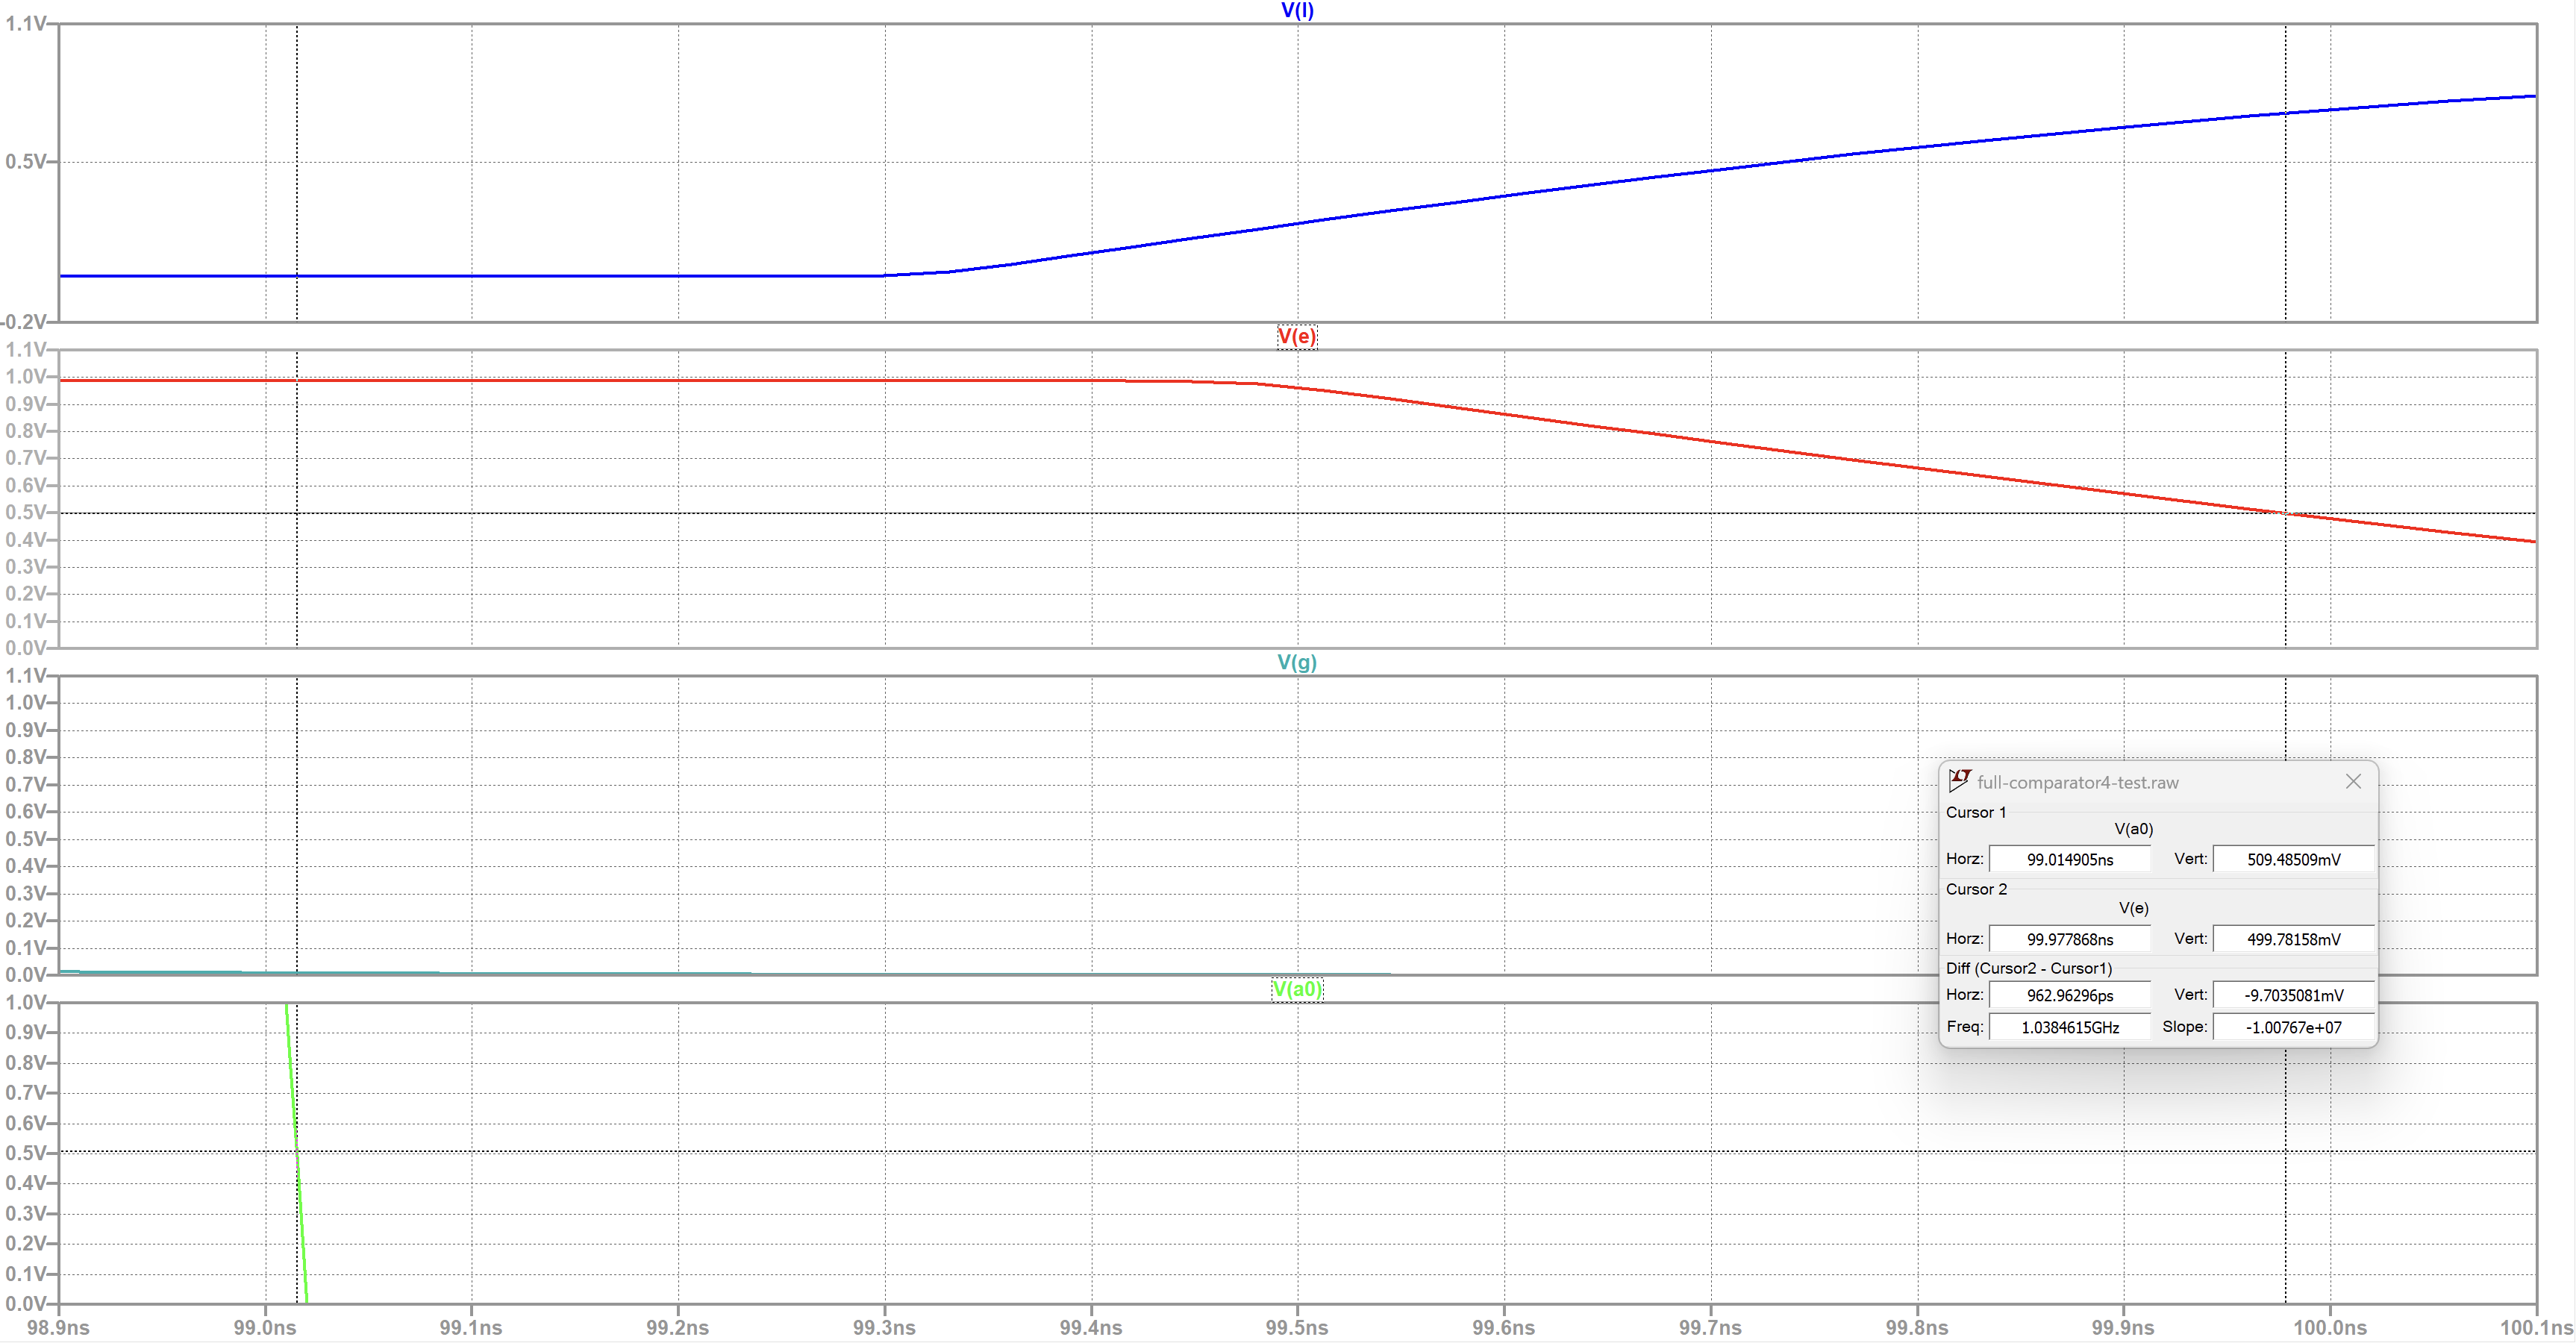
\includegraphics[width=\textwidth]{image/full-comparator-test-eq-10.png}
    \caption{Подсчет задержки распространения сигнала для 1-0 на выходе equal}
\end{figure}
$$t_{\text{pd}} = 99.977 - 99.015 = 0.963 ns$$
\begin{figure}[H]
    \centering
    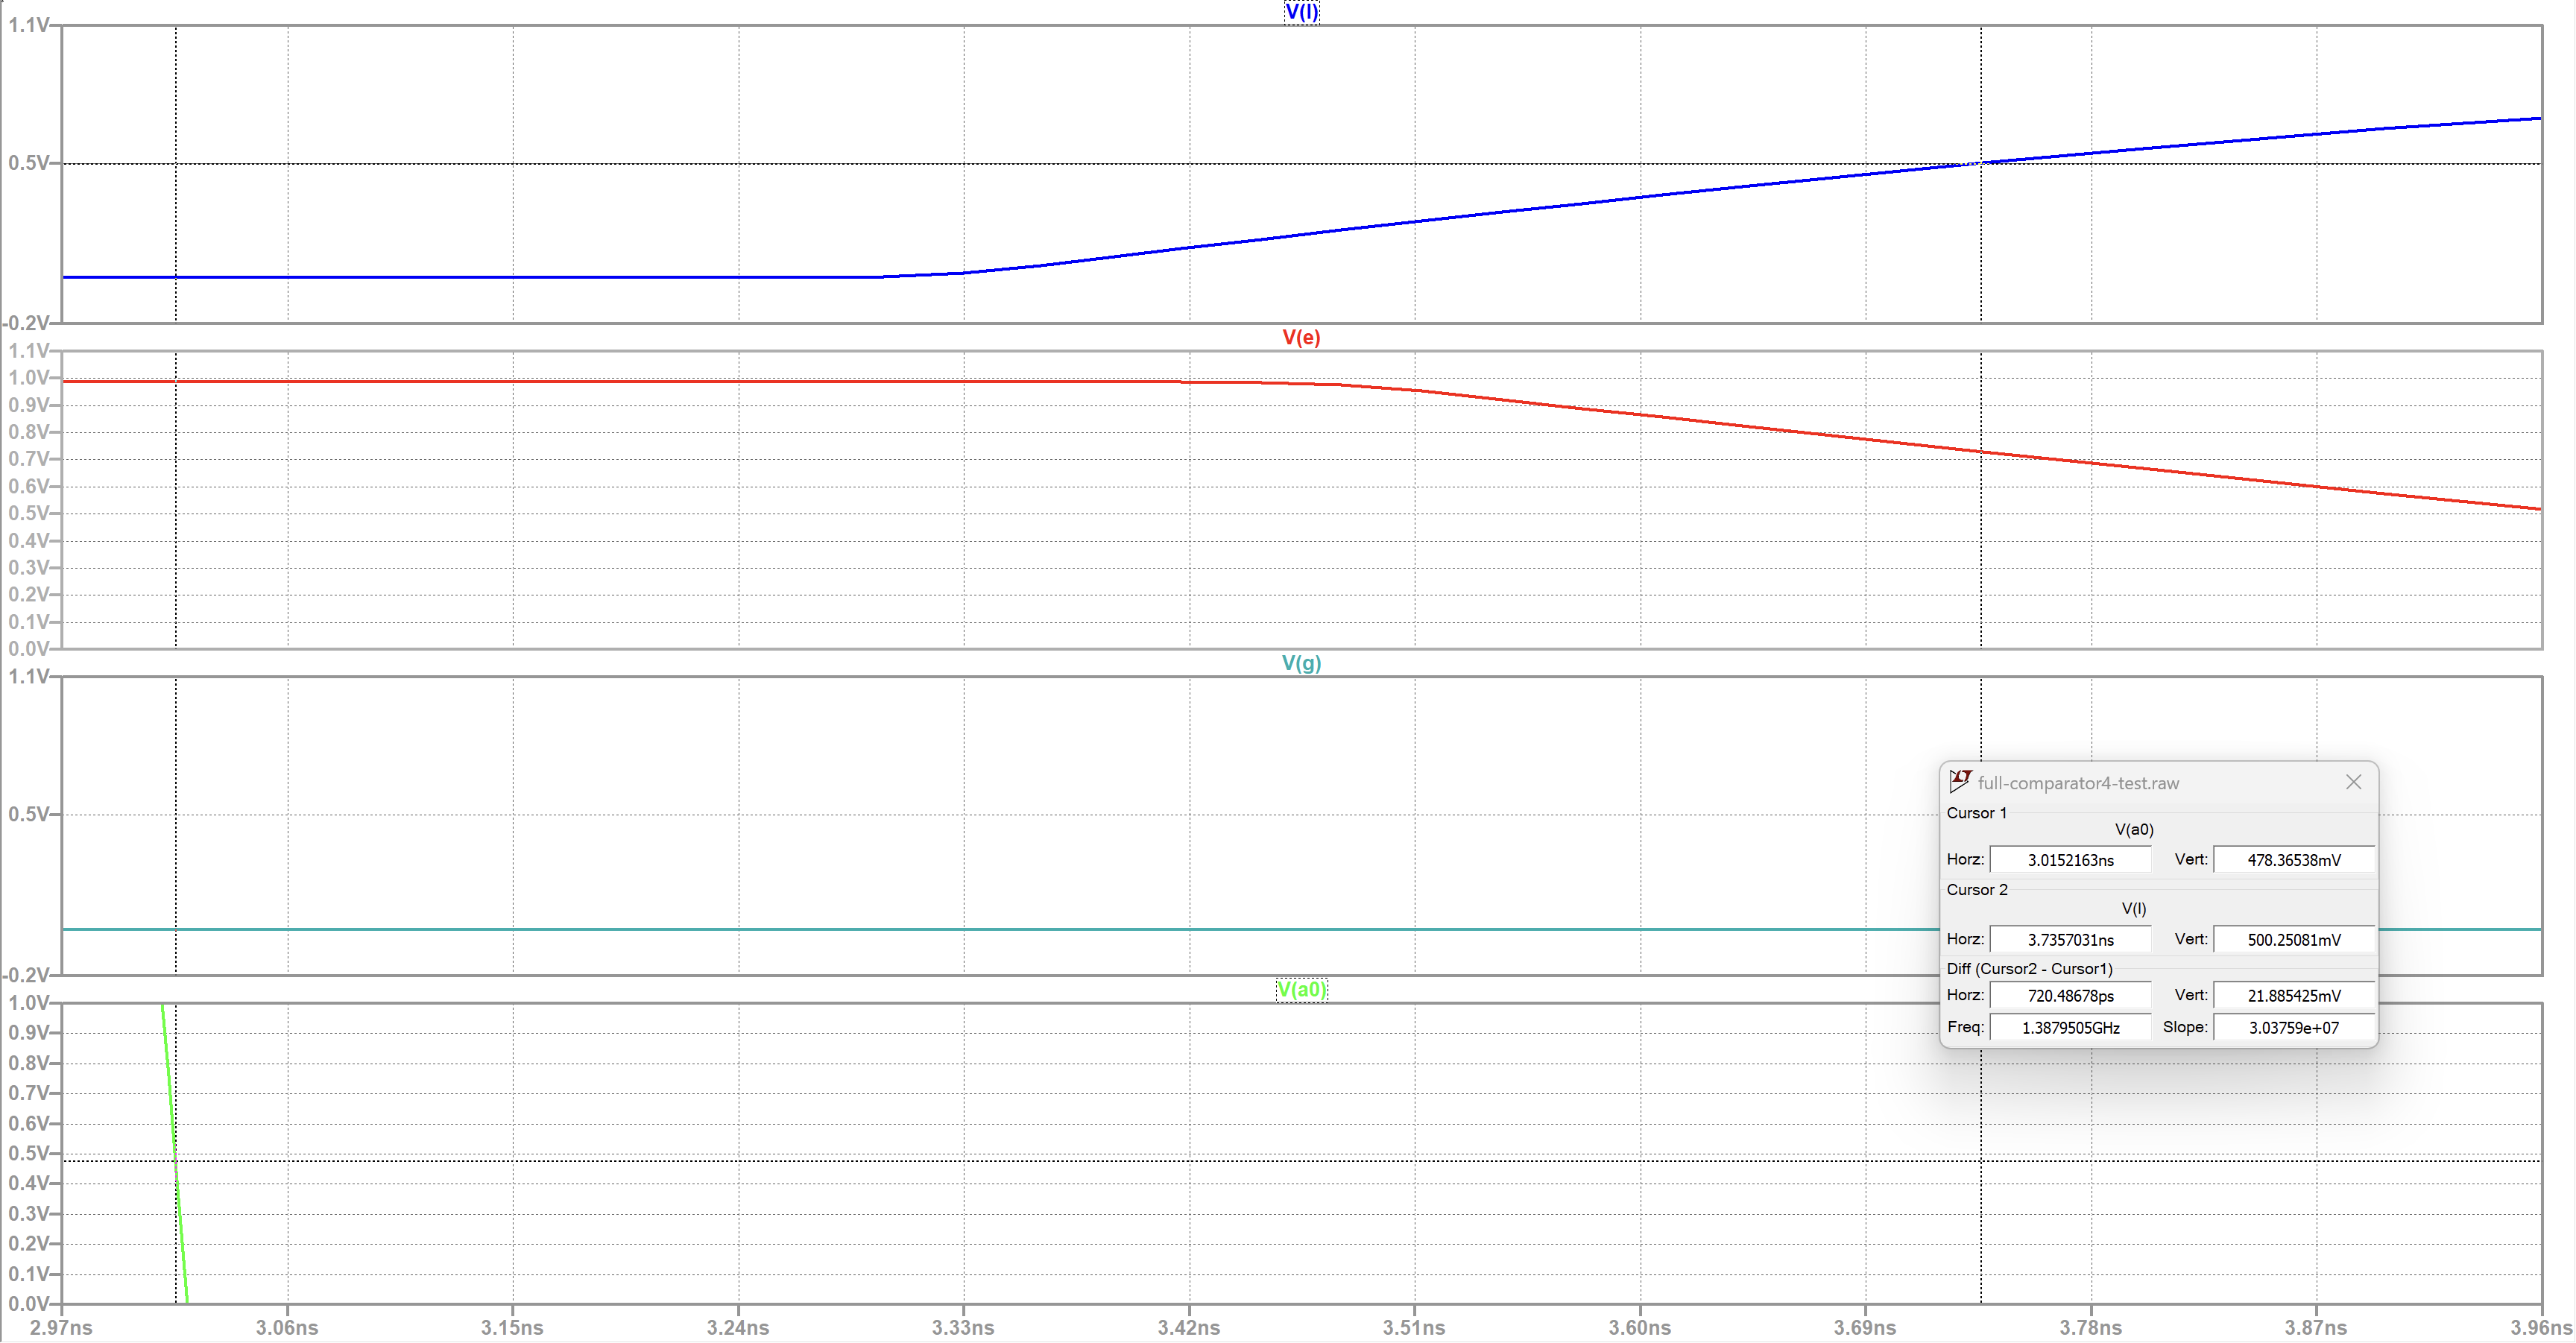
\includegraphics[width=\textwidth]{image/full-comparator-test-less-01.png}
    \caption{Подсчет задержки распространения сигнала для 0-1 на выходе less}
\end{figure}
$$t_{\text{pd}} = 3.736 - 3.015 = 0.720 ns$$
\begin{figure}[H]
    \centering
    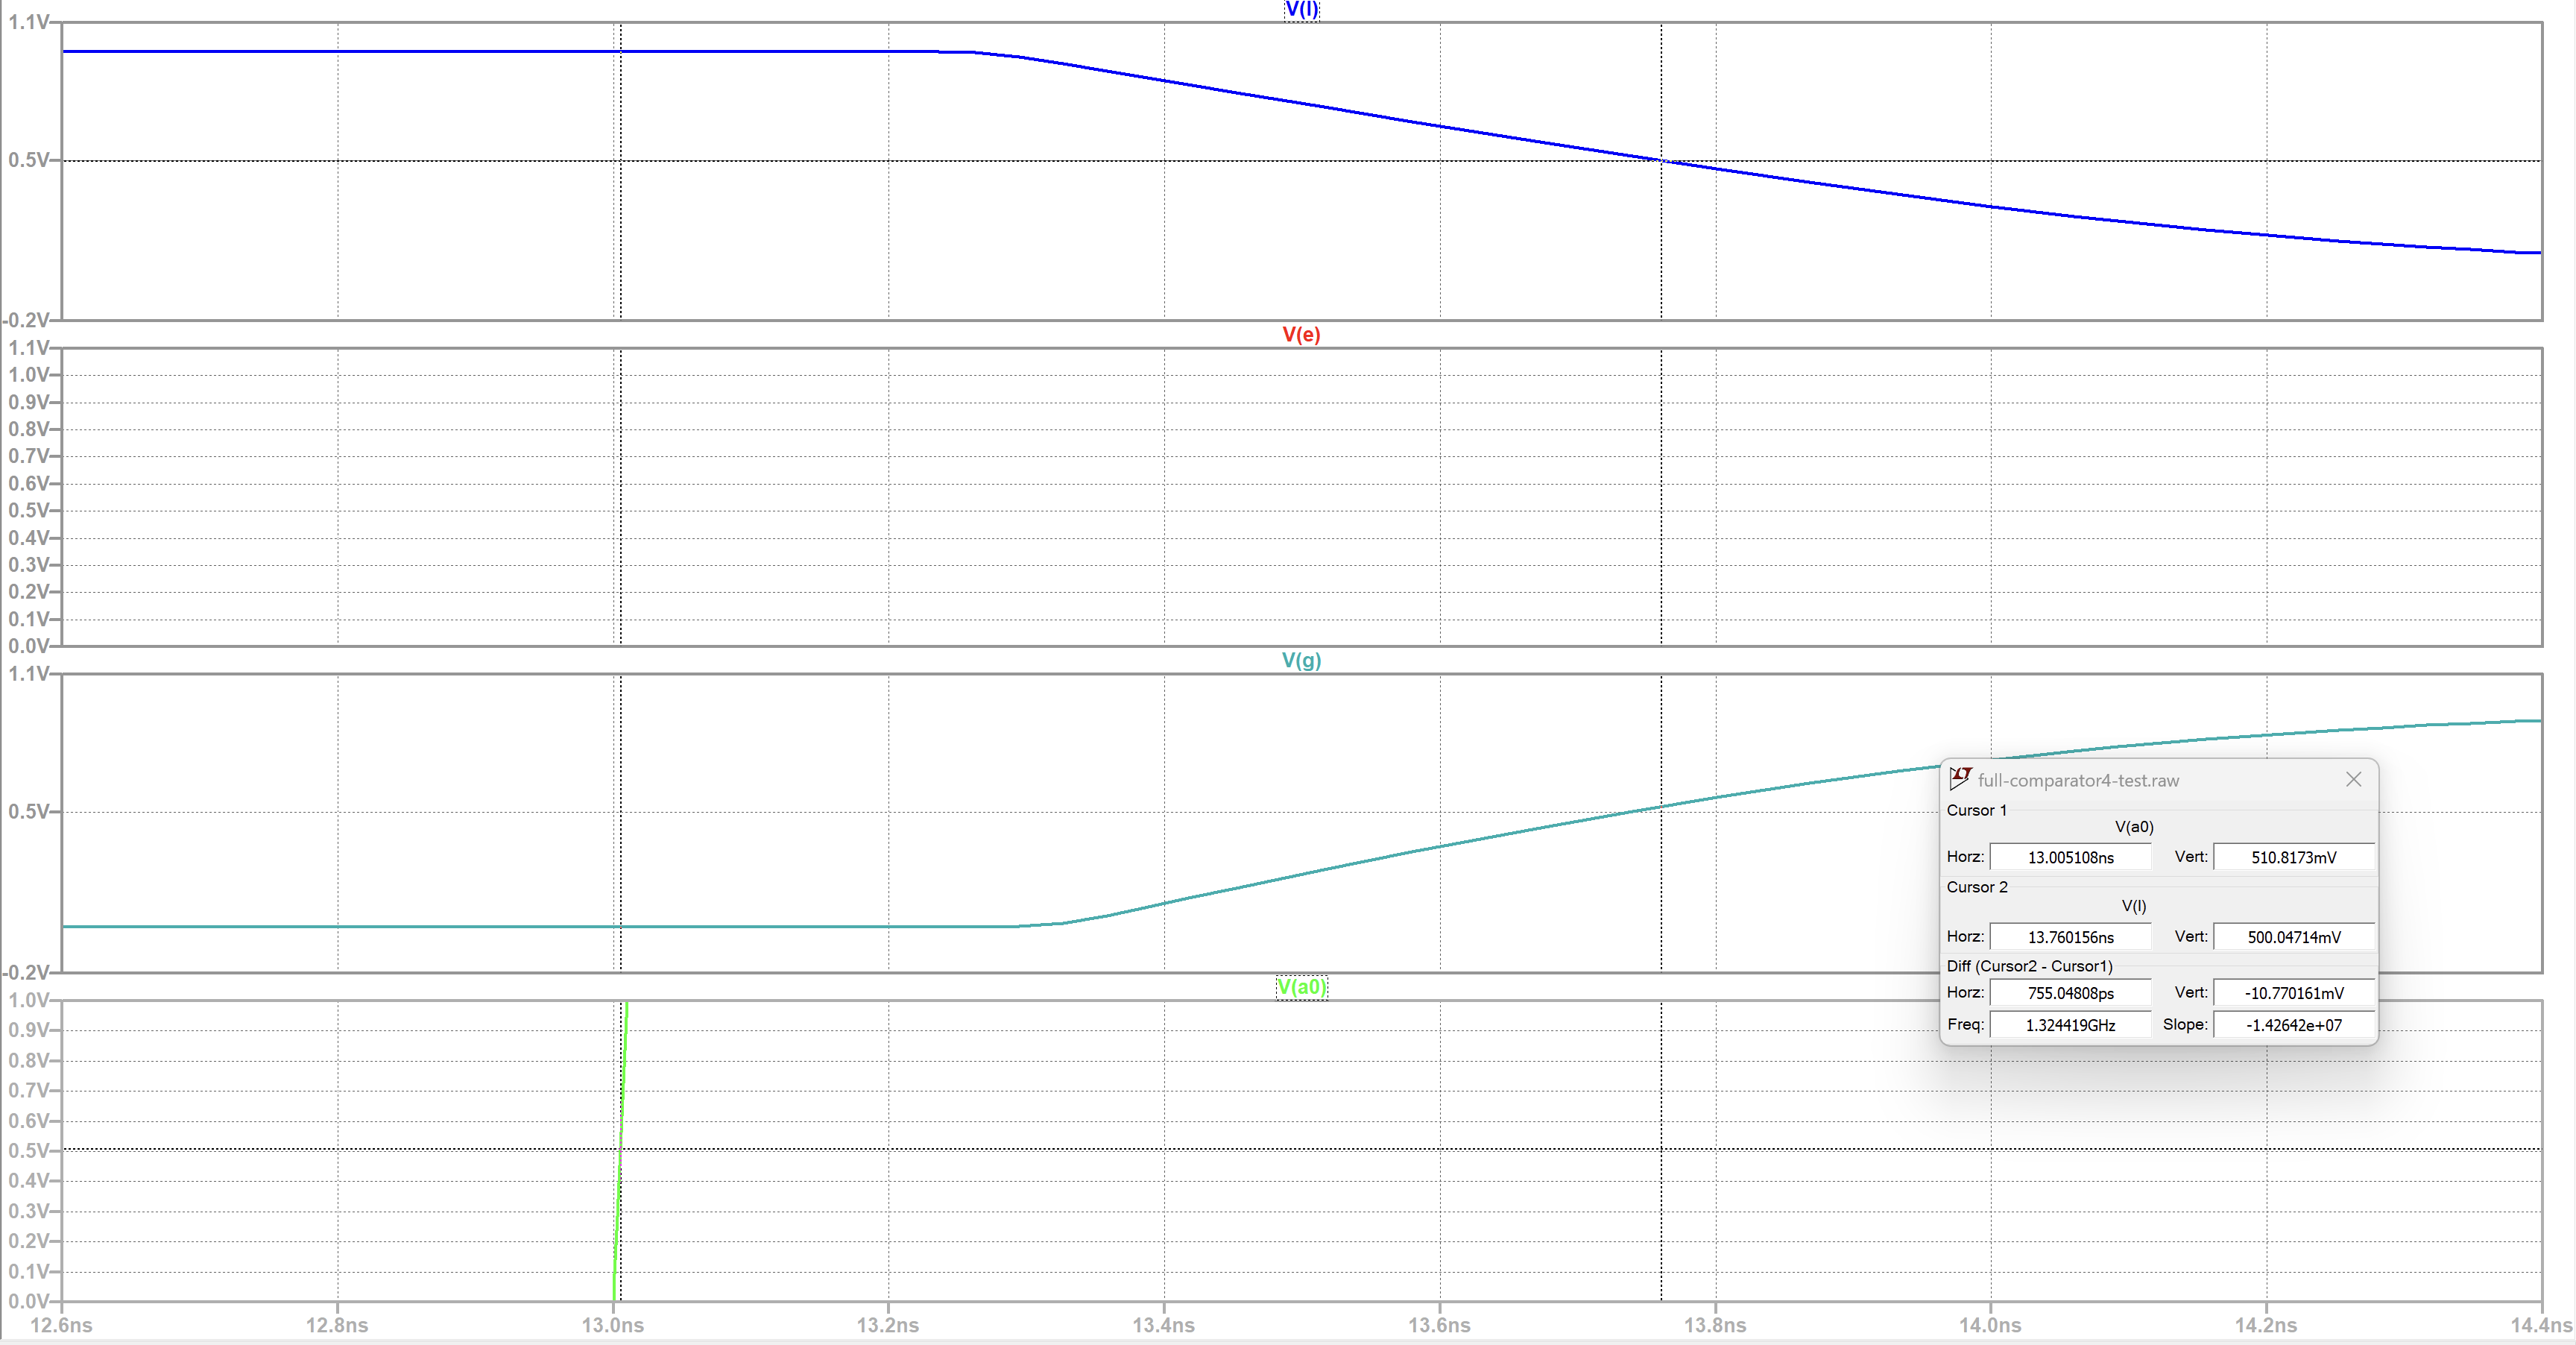
\includegraphics[width=\textwidth]{image/full-comparator-test-less-10.png}
    \caption{Подсчет задержки распространения сигнала для 1-0 на выходе less}
\end{figure}
$$t_{\text{pd}} = 13.760 - 13.005 = 0.755 ns$$
\begin{figure}[H]
    \centering
    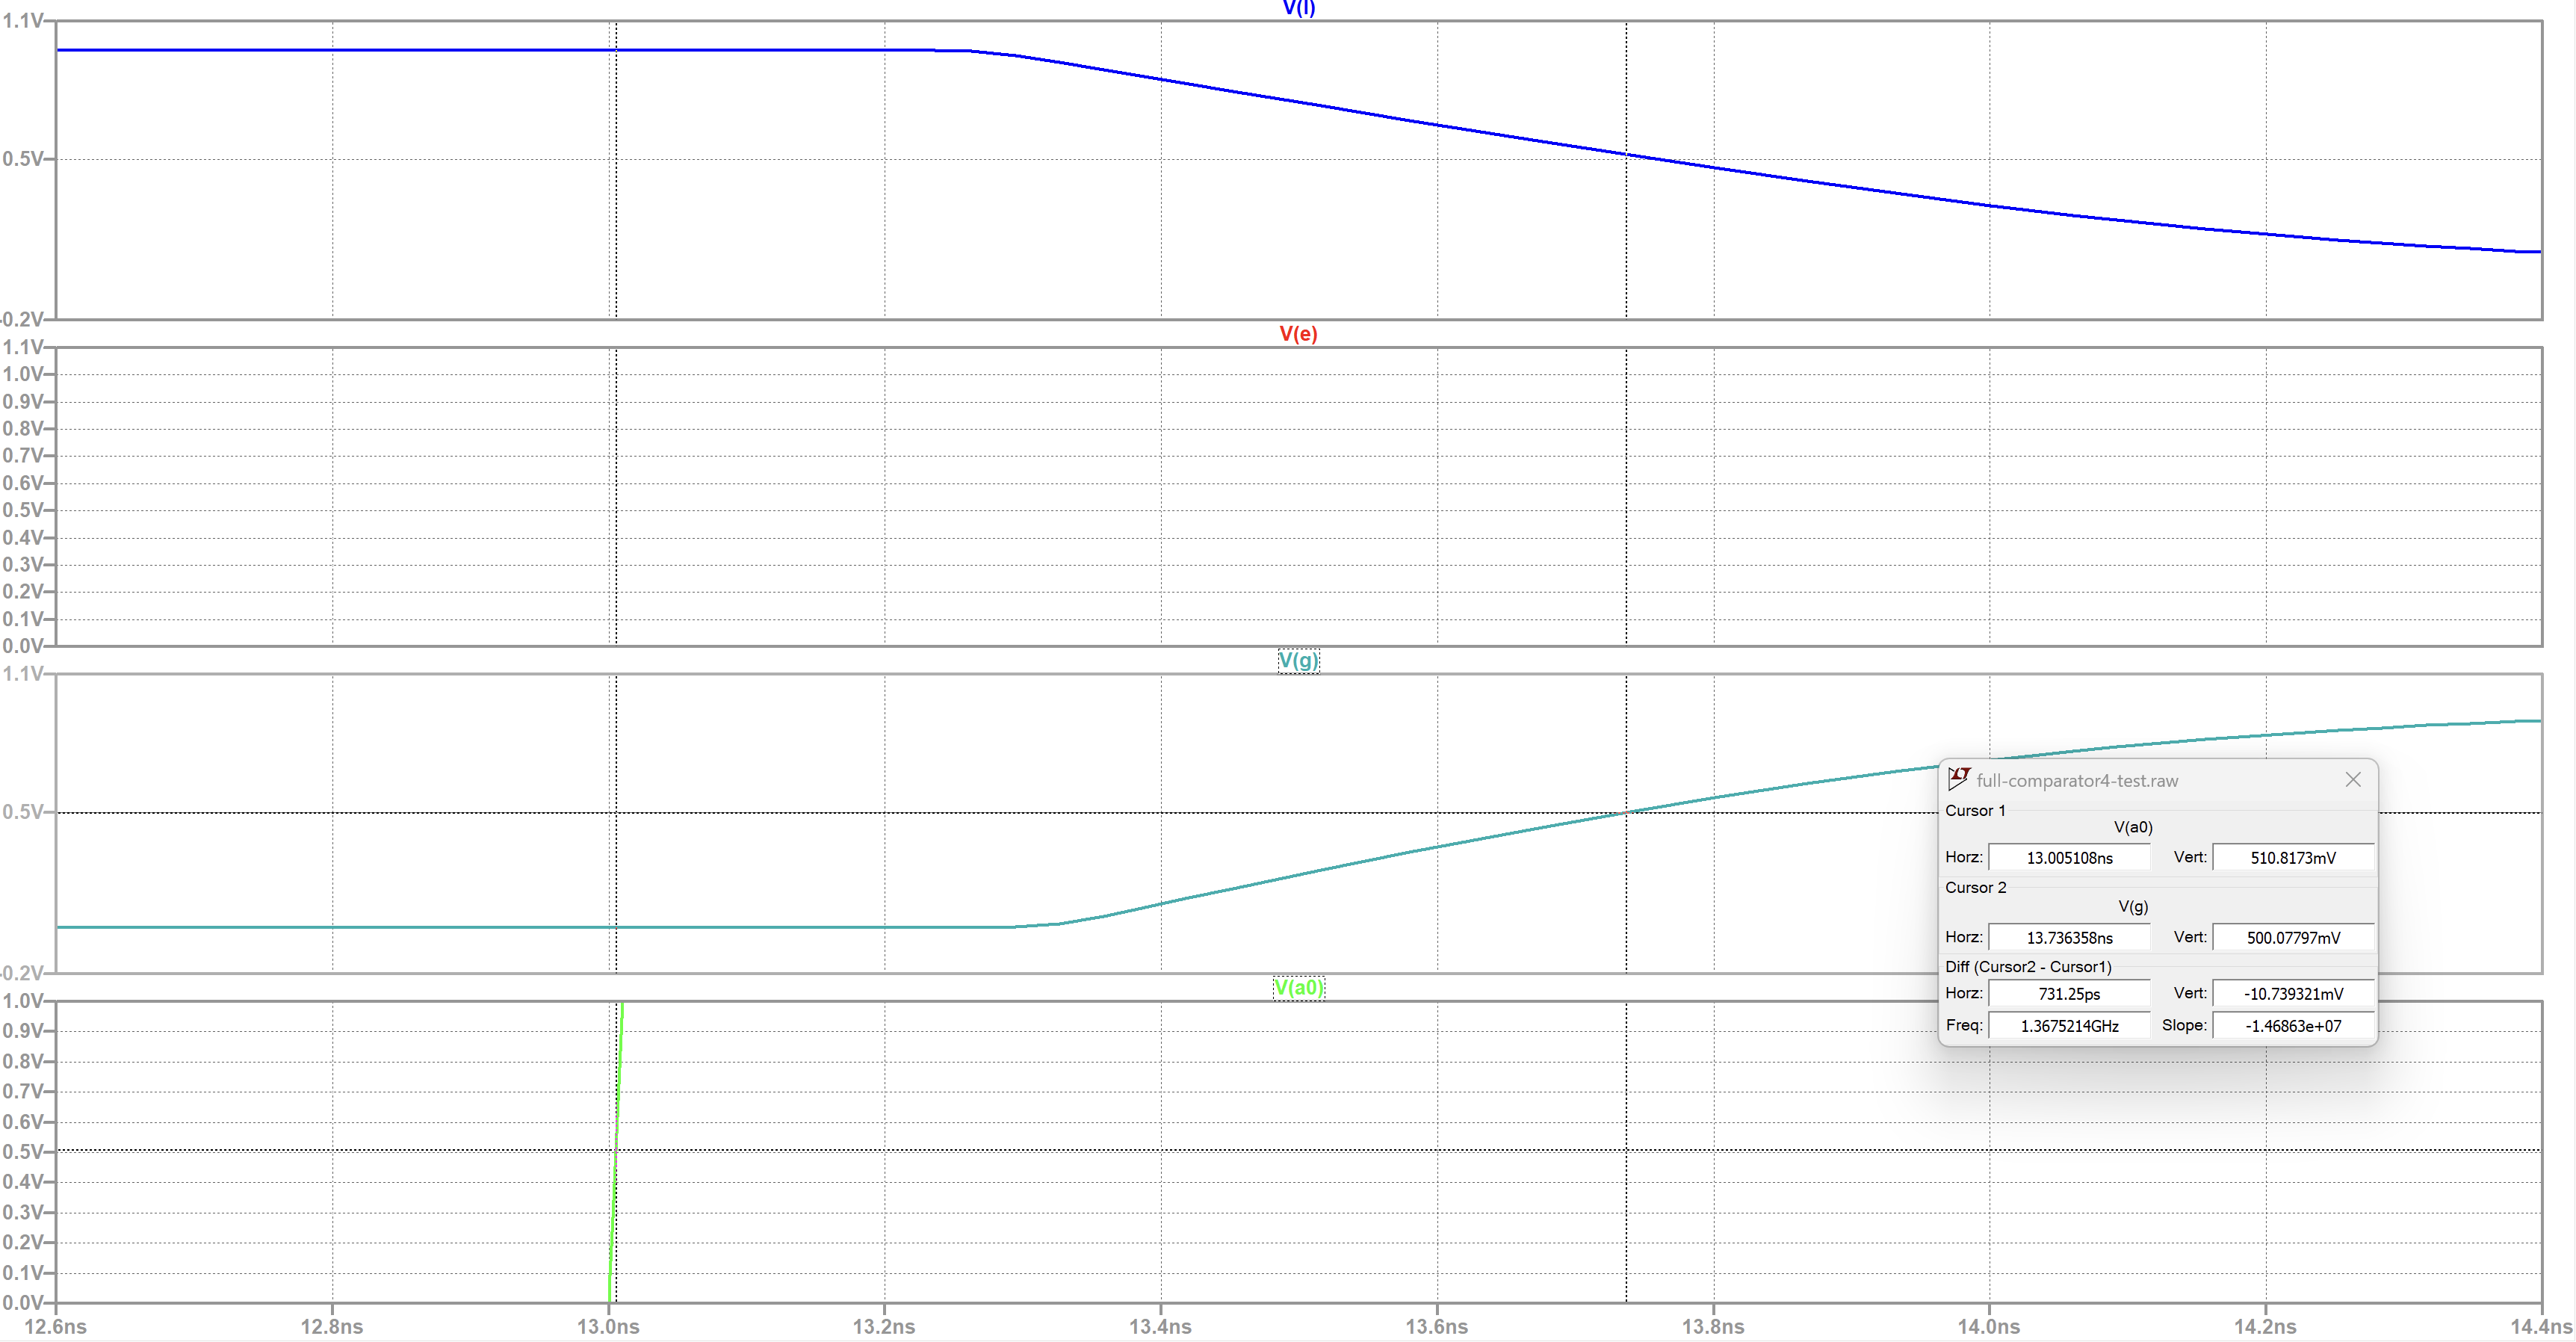
\includegraphics[width=\textwidth]{image/full-comparator-test-gt-01.png}
    \caption{Подсчет задержки распространения сигнала для 0-1 на выходе greater}
\end{figure}
$$t_{\text{pd}} = 13.736 - 13.005 = 0.731 ns$$
\begin{figure}[H]
    \centering
    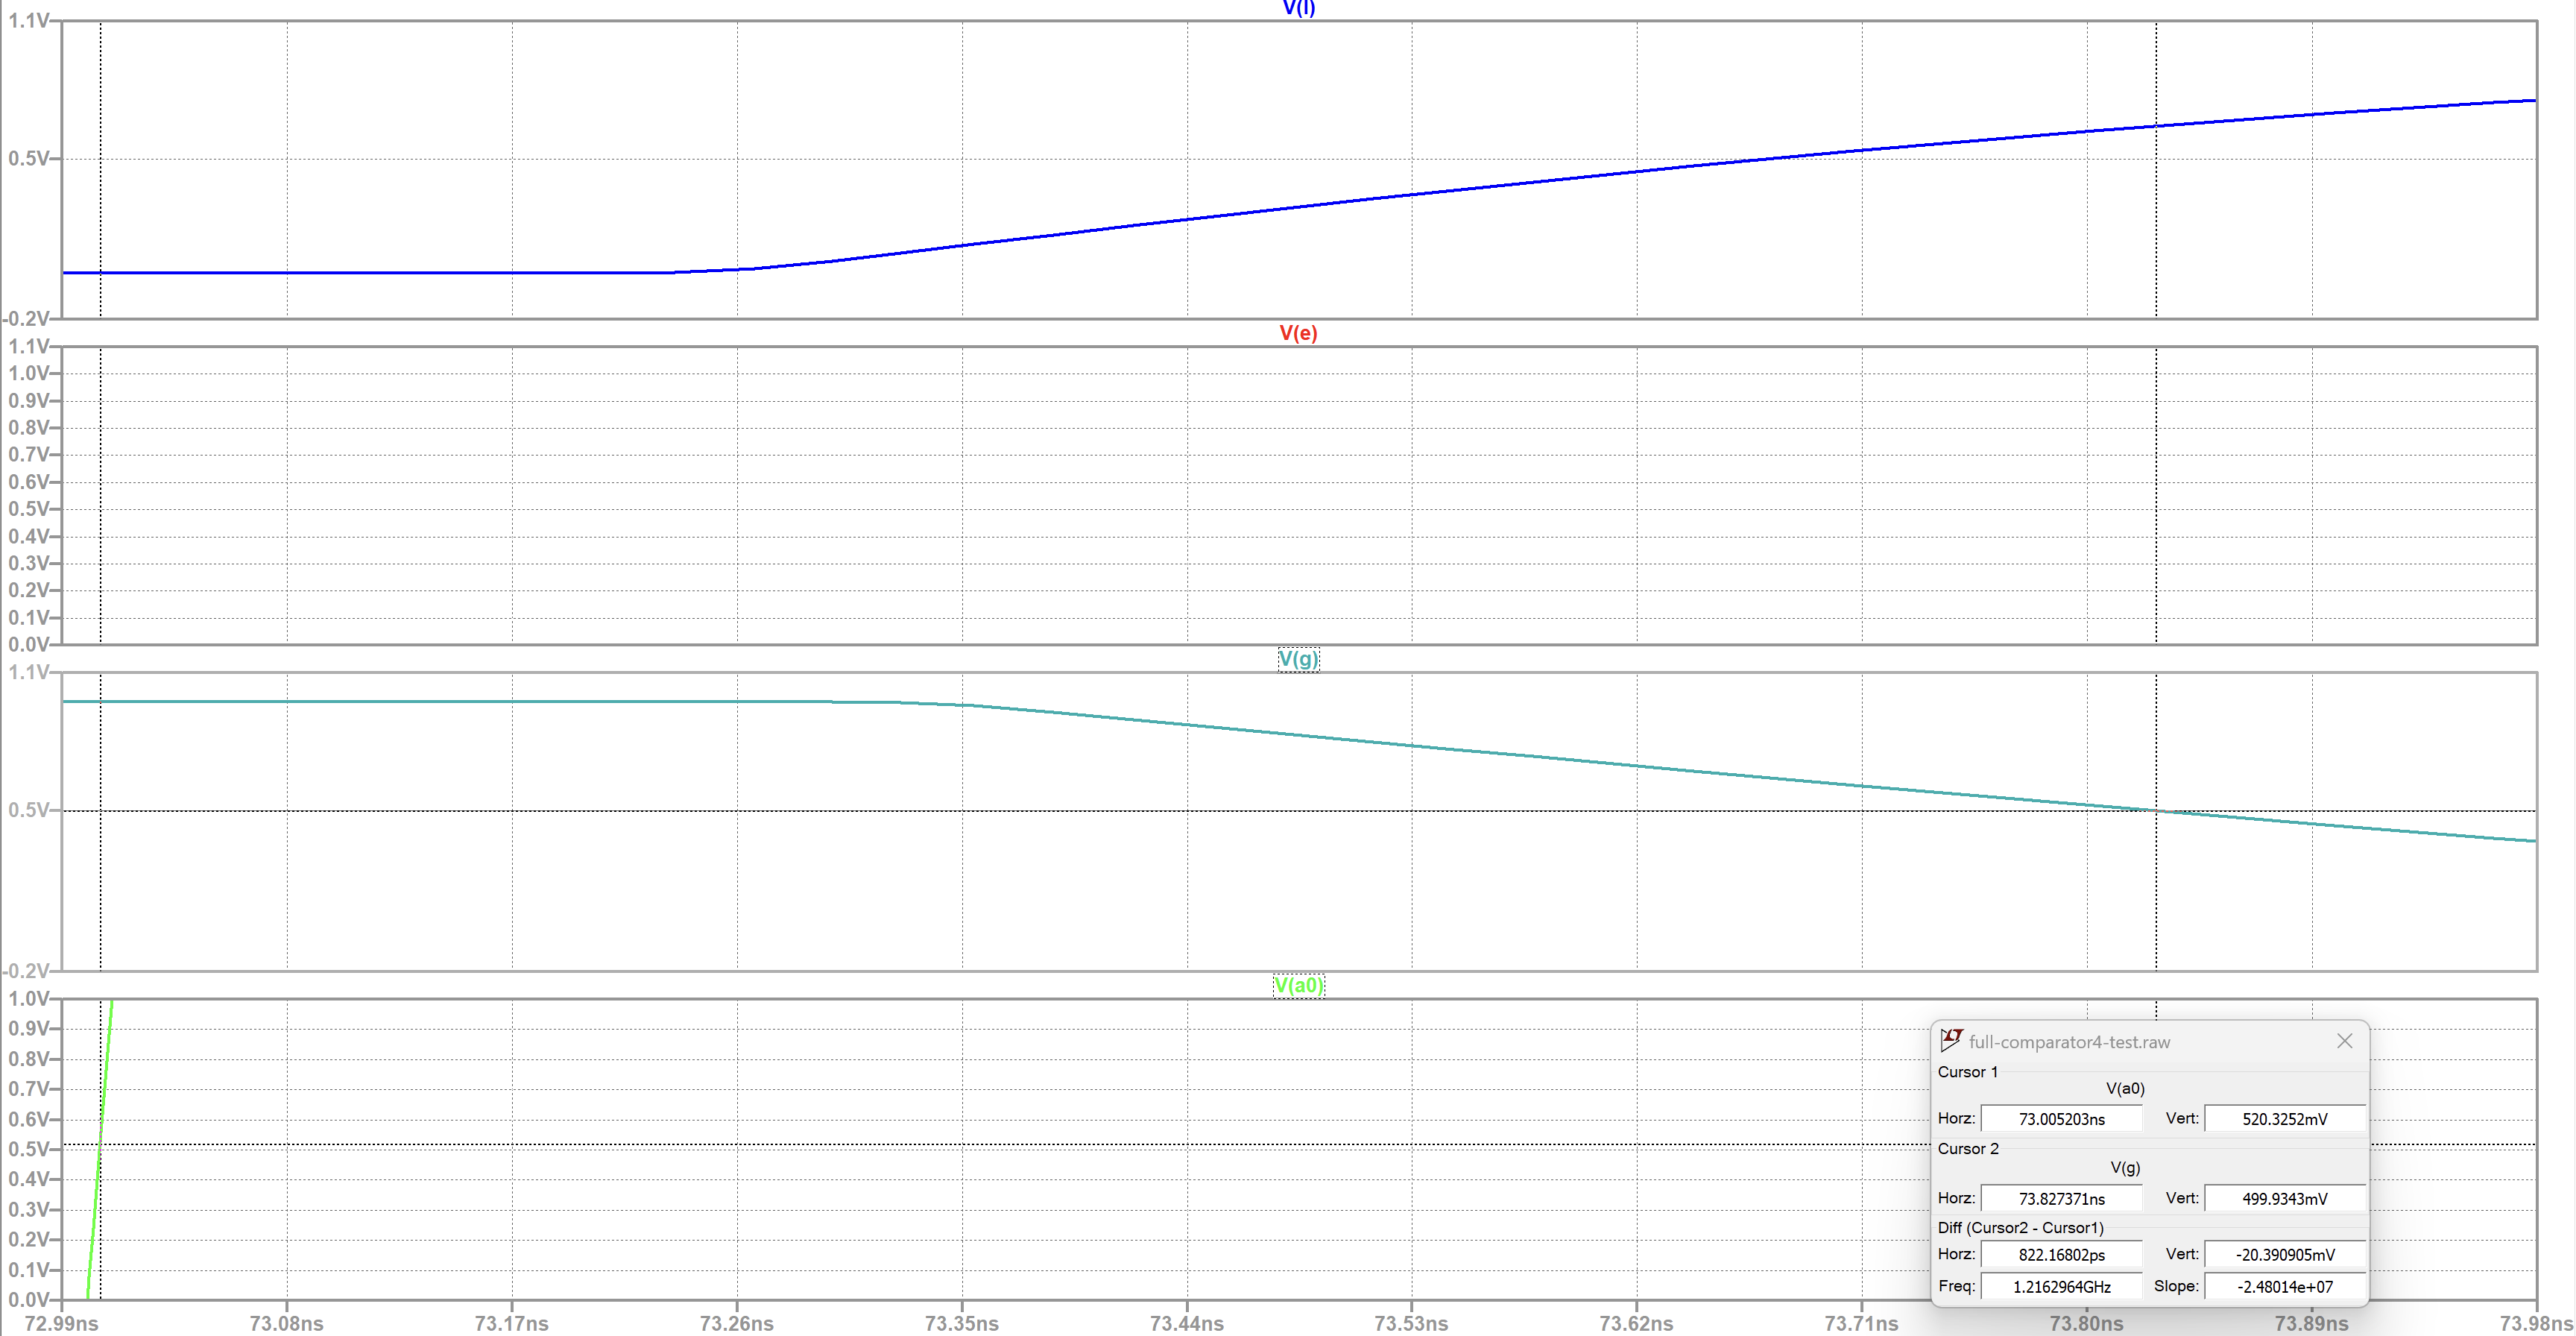
\includegraphics[width=\textwidth]{image/full-comparator-test-gt-10.png}
    \caption{Подсчет задержки распространения сигнала для 1-0 на выходе greater}
\end{figure}
$$t_{\text{pd}} = 73.827 - 73.005 = 0.822 ns$$
\subsection{Максимальная частота работы БОЭ.}

Тогда максимальная частота схемы:
$$ \nu_{\max} = \frac{1}{\max(t)}= \frac{1}{0.963} = 1.038\text{ГГц}$$


Поступим также как для NAND возьмем конденсатор с емкостью 0 фаррад.
\begin{figure}[H]
    \centering
    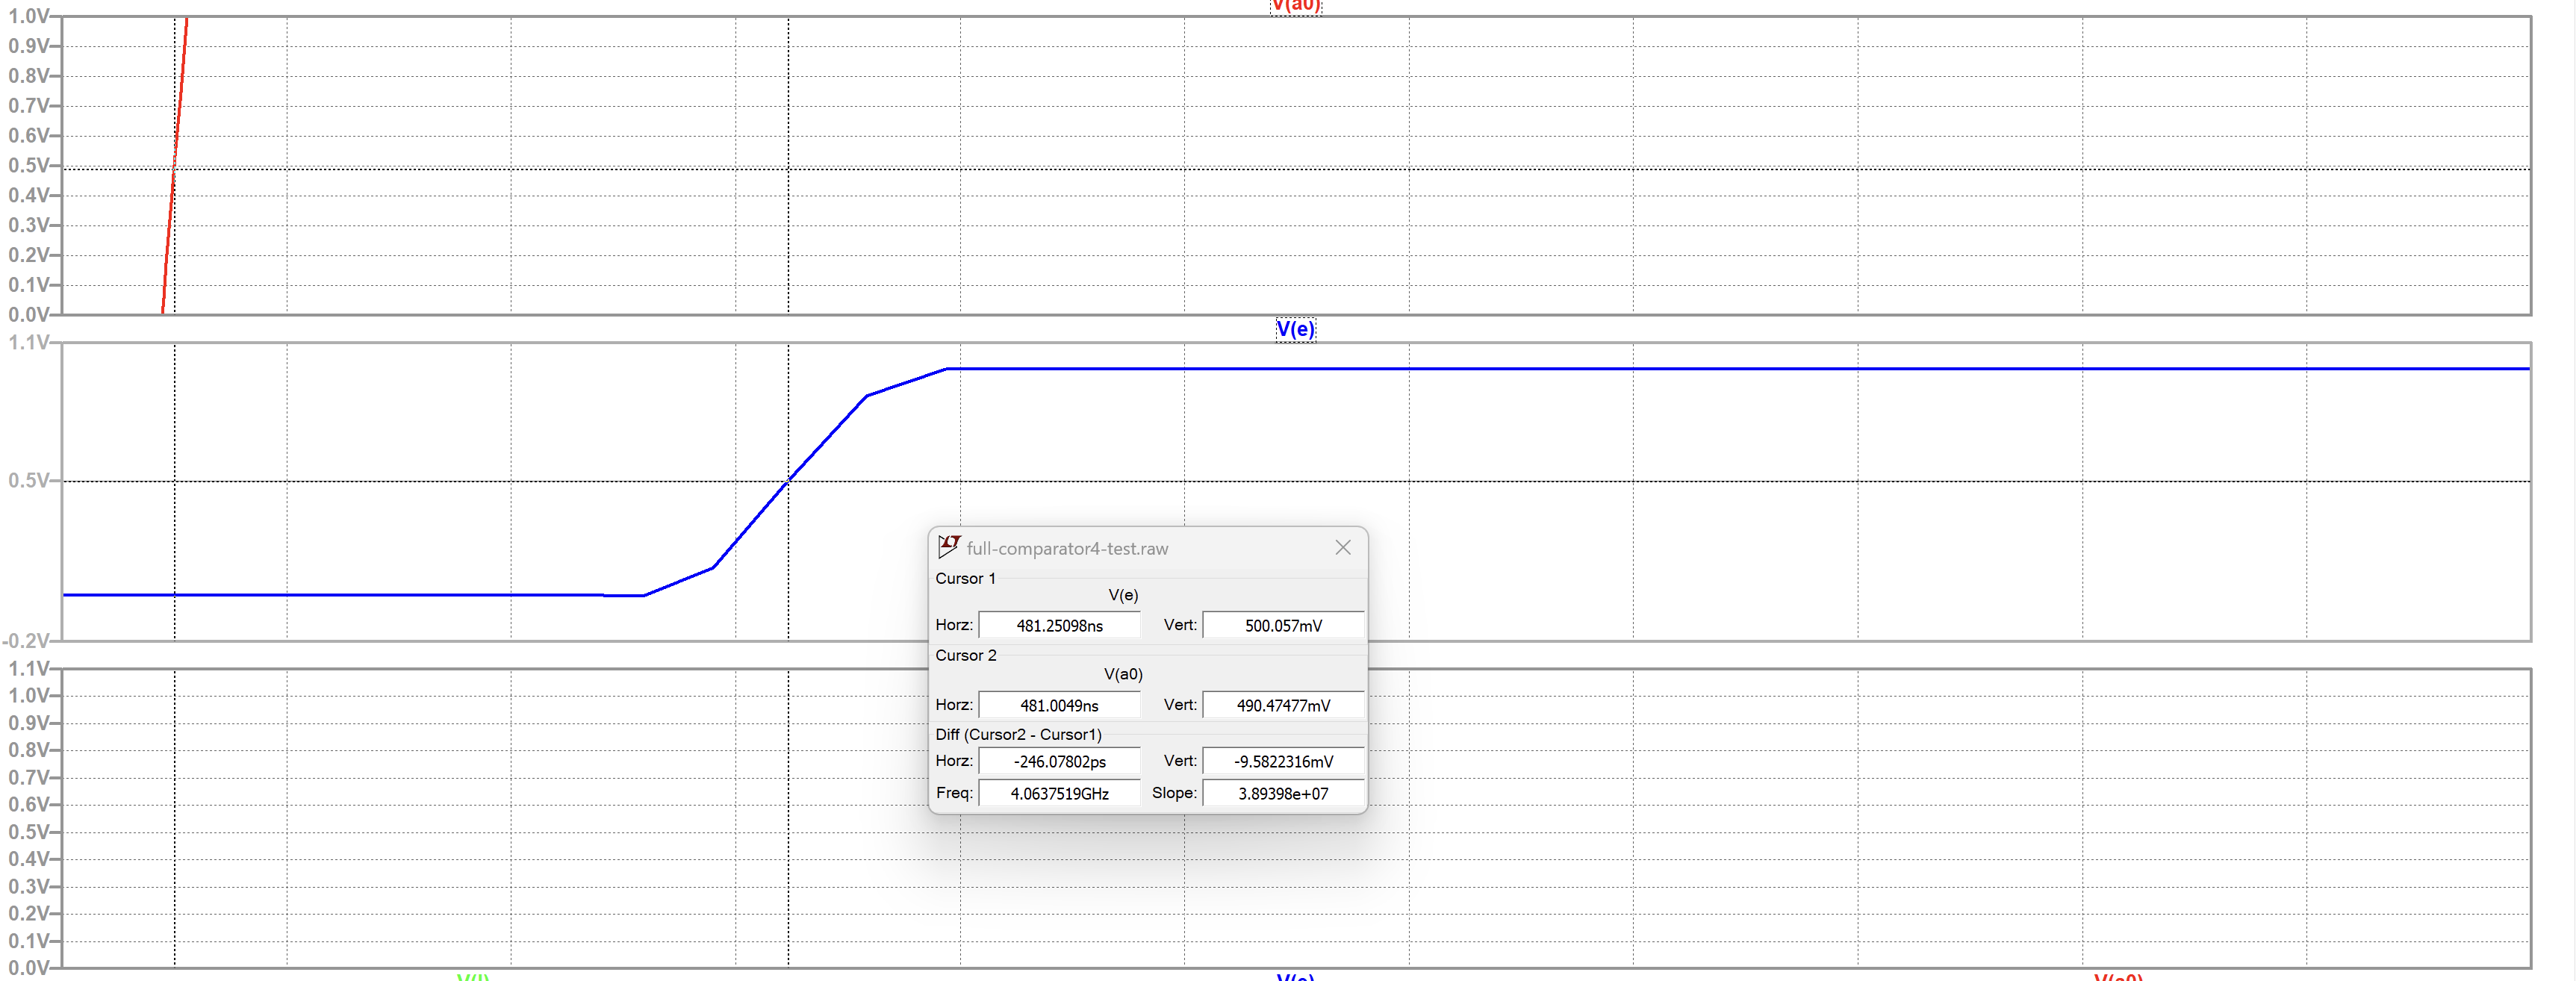
\includegraphics[width=\textwidth]{image/rise-2.png}
\end{figure}
\begin{figure}[H]
    \centering
    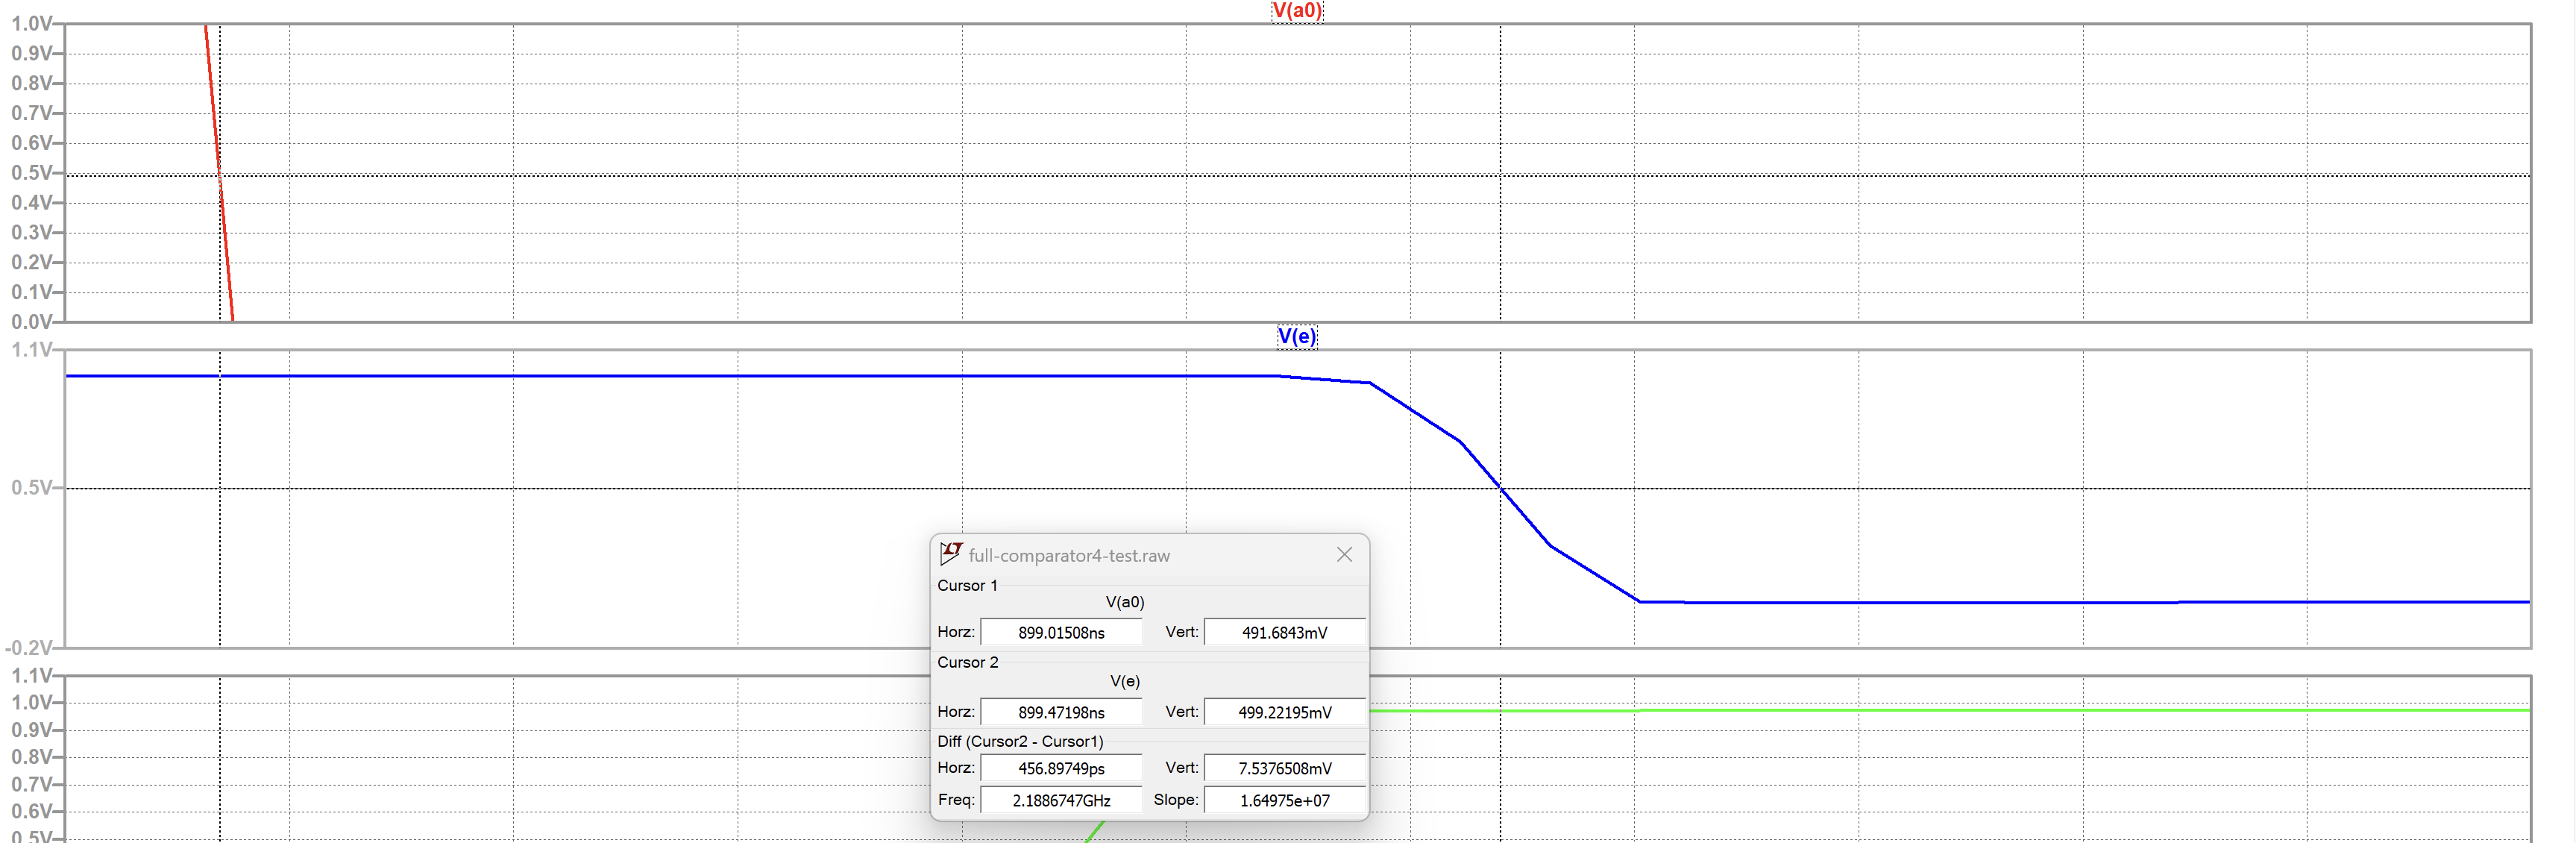
\includegraphics[width=\textwidth]{image/fall-2.png}
\end{figure}
$$t_{\text{rise}} = 246 ps$$

$$t_{\text{fall}} = 456.89 ps$$

Эти значения близки к теоритическим: Количество NAND $\cdot$ Задержка одного = $9 \cdot 4 \cdot 8 = 288 ps $ для  rise
$9 \cdot 4 \cdot 12 = 432 ps $ для  fall
Тогда максимальная частота схемы:
$$ \nu_{\max} = \frac{1}{\max(t)}= \frac{1}{0.432} = 2.31\text{ГГц}$$

\section{Отчет о выполнении заданий части 2:}
\subsection{Код разработанного модуля БОЭ}
\begin{lstlisting}[style=verilog, language=Verilog]
`timescale 1ns / 1ps

module full_comparator(
    input wire a, b,
    output wire l, e, g
    );
wire not_a, not_b;
wire v1_1, v1_2, v2_1;

nand(not_a, a, a);
nand(not_b, b, b);
nand(v1_1, not_a, b);
nand(v1_2, not_b, a);

nand(l, v1_1, v1_1);

nand(v2_1, v1_1, v1_2);
nand(e, v2_1, v2_1);

nand(g, v1_2, v1_2);

endmodule

module and2(
    input wire a, b,
    output wire out
    );
wire ab;
nand(ab, a, b);
nand(out, ab, ab);

endmodule

module and3(
    input wire a, b, c,
    output wire out
    );

wire ab, not_ab, abc;
nand(ab, a, b);
nand(not_ab, ab, ab);
nand(abc, not_ab, c);
nand(out, abc, abc);
endmodule

module or2(
    input wire a, b,
    output wire out
    );
wire not_a, not_b;
nand(not_a, a, a);
nand(not_b, b, b);

nand(out, not_a, not_b);
endmodule

module full_comparator_seq(
    input wire a, b, fl, fe, fg,
    output wire l, e, g
);

wire not_fl, not_fg, fc_l, fc_e, fc_g, add3_out, andl_out, andg_out;
nand(not_fl, fl, fl);
nand(not_fg, fg, fg);

full_comparator fc_i(.a(a), .b(b), .l(fc_l), .e(fc_e), .g(fc_g));
and3 and3_i(.a(not_fl), .b(fe), .c(not_fg), .out(add3_out));

and2 and2_i1(.a(fc_l), .b(add3_out), .out(andl_out));
and2 and2_i2(.a(fc_e), .b(add3_out), .out(e));
and2 and2_i3(.a(fc_g), .b(add3_out), .out(andg_out));

or2 or_i1(.a(andl_out), .b(fl), .out(l));
or2 or_i2(.a(andg_out), .b(fg), .out(g));

endmodule



module full_comparator4(
    input wire[0:3] a,
    input wire[0:3] b,
    input fl, fe, fg,
    output l, e, g
    );
wire[2:0] fcsl_out, fcse_out, fcsg_out;
full_comparator_seq fcs1(a[0],b[0],fl,fe,fg,fcsl_out[0],fcse_out[0],fcsg_out[0]);
full_comparator_seq fcs2(a[1],b[1],fcsl_out[0],fcse_out[0],fcsg_out[0], fcsl_out[1],fcse_out[1],fcsg_out[1]);
full_comparator_seq fcs3(a[2],b[2],fcsl_out[1],fcse_out[1],fcsg_out[1], fcsl_out[2],fcse_out[2],fcsg_out[2]);
full_comparator_seq fcs4(a[3],b[3],fcsl_out[2],fcse_out[2],fcsg_out[2],l,e,g);    
endmodule

\end{lstlisting}

\subsection{Код разработанного тестового окружения}
\begin{lstlisting}[style=verilog, language=Verilog]
`timescale 1ns / 1ps //reference time / precision


module full_comparator4_tb;
//inputs
reg[3:0] a, b;
reg fl, fe, fg;
//outputs
wire l;
wire e;
wire g;

// Unit under test (UUT)

full_comparator4 uut(a, b, fl, fe, fg, l, e, g);

//32 bit integer
integer i, j;

reg[3:0] expr_lt, expr_eq, expr_gt;

initial
begin
{fl, fe, fg} = 3'b010;
    for (i = 0; i < 16; i = i + 1) begin
        a = i;
        for (j = 0; j < 16; j = j + 1) begin
            b = j;
            expr_lt = ( i < j );
            expr_eq = ( i == j );
            expr_gt = ( i > j );
            #10;
            if (l == expr_lt & e == expr_eq & g == expr_gt) begin
                $display("[CORRECT]: a = %d, b = %d, l = %d, e = %d, g = %d", a, b, l, e, g);
            end else begin
                 $display("[INCORRECT]: a=%d, b=%d, expr_lt=%d, expr_eq=%d, expr_gt=%d, l=%d, e=%d, g=%d",
                 a, b, expr_lt, expr_eq, expr_gt, l, e, g);
            end
        end
    end
$stop;
end


endmodule

\end{lstlisting}

\subsection{Временная диаграмма процесса тестирования БОЭ}
\begin{figure}[H]
    \centering
    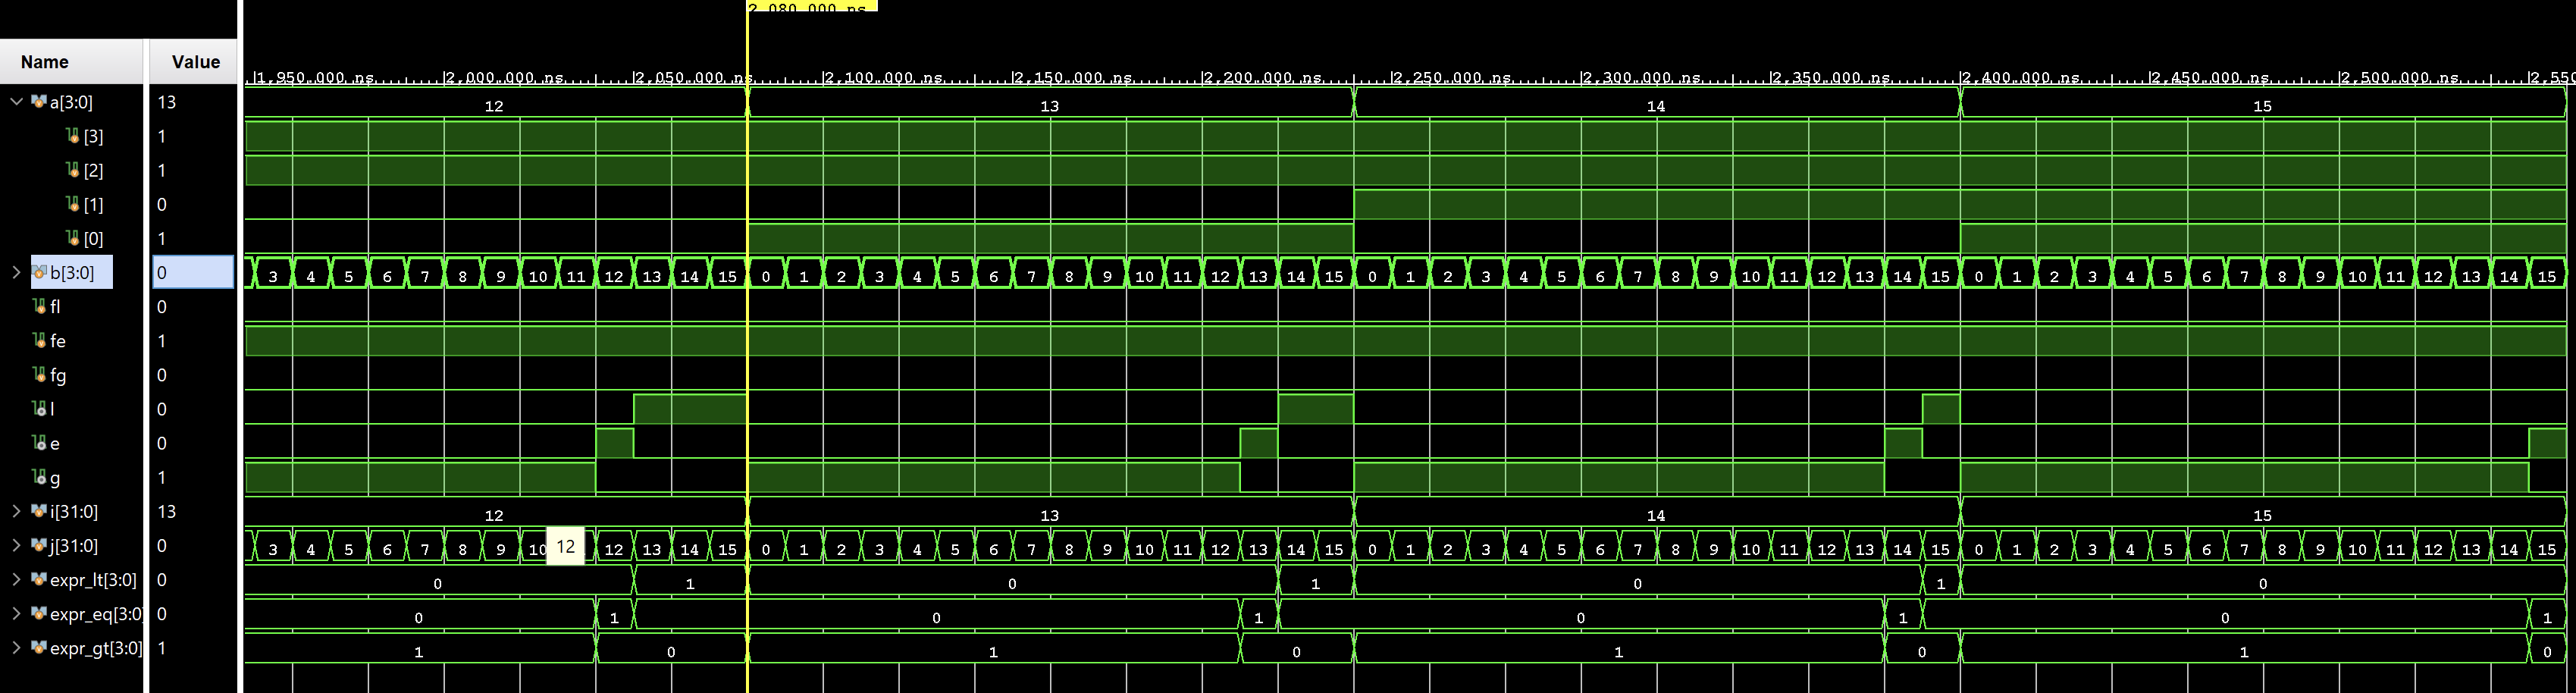
\includegraphics[width=\textwidth]{image/verilog-diagram.png}
    \caption{Отрывок временная диаграммы процесса тестирования БОЭ}
\end{figure}

Логи

\begin{lstlisting}[style=verilog, language=Verilog]
[CORRECT]: a =  6, b =  4, l = 0, e = 0, g = 1
[CORRECT]: a =  6, b =  5, l = 0, e = 0, g = 1
[CORRECT]: a =  6, b =  6, l = 0, e = 1, g = 0
[CORRECT]: a =  6, b =  7, l = 1, e = 0, g = 0
[CORRECT]: a =  6, b =  8, l = 1, e = 0, g = 0
[CORRECT]: a =  6, b =  9, l = 1, e = 0, g = 0
[CORRECT]: a =  6, b = 10, l = 1, e = 0, g = 0
[CORRECT]: a =  6, b = 11, l = 1, e = 0, g = 0
[CORRECT]: a =  6, b = 12, l = 1, e = 0, g = 0
[CORRECT]: a =  6, b = 13, l = 1, e = 0, g = 0
[CORRECT]: a =  6, b = 14, l = 1, e = 0, g = 0
[CORRECT]: a =  6, b = 15, l = 1, e = 0, g = 0
[CORRECT]: a =  7, b =  0, l = 0, e = 0, g = 1
[CORRECT]: a =  7, b =  1, l = 0, e = 0, g = 1
[CORRECT]: a =  7, b =  2, l = 0, e = 0, g = 1
[CORRECT]: a =  7, b =  3, l = 0, e = 0, g = 1
[CORRECT]: a =  7, b =  4, l = 0, e = 0, g = 1
[CORRECT]: a =  7, b =  5, l = 0, e = 0, g = 1
[CORRECT]: a =  7, b =  6, l = 0, e = 0, g = 1
[CORRECT]: a =  7, b =  7, l = 0, e = 1, g = 0
[CORRECT]: a =  7, b =  8, l = 1, e = 0, g = 0
[CORRECT]: a =  7, b =  9, l = 1, e = 0, g = 0
[CORRECT]: a =  7, b = 10, l = 1, e = 0, g = 0
[CORRECT]: a =  7, b = 11, l = 1, e = 0, g = 0
[CORRECT]: a =  7, b = 12, l = 1, e = 0, g = 0
[CORRECT]: a =  7, b = 13, l = 1, e = 0, g = 0
[CORRECT]: a =  7, b = 14, l = 1, e = 0, g = 0
[CORRECT]: a =  7, b = 15, l = 1, e = 0, g = 0
[CORRECT]: a =  8, b =  0, l = 0, e = 0, g = 1
[CORRECT]: a =  8, b =  1, l = 0, e = 0, g = 1
[CORRECT]: a =  8, b =  2, l = 0, e = 0, g = 1
[CORRECT]: a =  8, b =  3, l = 0, e = 0, g = 1
[CORRECT]: a =  8, b =  4, l = 0, e = 0, g = 1
[CORRECT]: a =  8, b =  5, l = 0, e = 0, g = 1
[CORRECT]: a =  8, b =  6, l = 0, e = 0, g = 1
[CORRECT]: a =  8, b =  7, l = 0, e = 0, g = 1
[CORRECT]: a =  8, b =  8, l = 0, e = 1, g = 0
[CORRECT]: a =  8, b =  9, l = 1, e = 0, g = 0
[CORRECT]: a =  8, b = 10, l = 1, e = 0, g = 0
[CORRECT]: a =  8, b = 11, l = 1, e = 0, g = 0
[CORRECT]: a =  8, b = 12, l = 1, e = 0, g = 0
[CORRECT]: a =  8, b = 13, l = 1, e = 0, g = 0
[CORRECT]: a =  8, b = 14, l = 1, e = 0, g = 0
[CORRECT]: a =  8, b = 15, l = 1, e = 0, g = 0
[CORRECT]: a =  9, b =  0, l = 0, e = 0, g = 1
[CORRECT]: a =  9, b =  1, l = 0, e = 0, g = 1
[CORRECT]: a =  9, b =  2, l = 0, e = 0, g = 1
[CORRECT]: a =  9, b =  3, l = 0, e = 0, g = 1
[CORRECT]: a =  9, b =  4, l = 0, e = 0, g = 1
[CORRECT]: a =  9, b =  5, l = 0, e = 0, g = 1
[CORRECT]: a =  9, b =  6, l = 0, e = 0, g = 1
[CORRECT]: a =  9, b =  7, l = 0, e = 0, g = 1
[CORRECT]: a =  9, b =  8, l = 0, e = 0, g = 1
[CORRECT]: a =  9, b =  9, l = 0, e = 1, g = 0
[CORRECT]: a =  9, b = 10, l = 1, e = 0, g = 0
[CORRECT]: a =  9, b = 11, l = 1, e = 0, g = 0
[CORRECT]: a =  9, b = 12, l = 1, e = 0, g = 0
[CORRECT]: a =  9, b = 13, l = 1, e = 0, g = 0
[CORRECT]: a =  9, b = 14, l = 1, e = 0, g = 0
[CORRECT]: a =  9, b = 15, l = 1, e = 0, g = 0
[CORRECT]: a = 10, b =  0, l = 0, e = 0, g = 1
[CORRECT]: a = 10, b =  1, l = 0, e = 0, g = 1
[CORRECT]: a = 10, b =  2, l = 0, e = 0, g = 1
[CORRECT]: a = 10, b =  3, l = 0, e = 0, g = 1
[CORRECT]: a = 10, b =  4, l = 0, e = 0, g = 1
[CORRECT]: a = 10, b =  5, l = 0, e = 0, g = 1
[CORRECT]: a = 10, b =  6, l = 0, e = 0, g = 1
[CORRECT]: a = 10, b =  7, l = 0, e = 0, g = 1
[CORRECT]: a = 10, b =  8, l = 0, e = 0, g = 1
[CORRECT]: a = 10, b =  9, l = 0, e = 0, g = 1
[CORRECT]: a = 10, b = 10, l = 0, e = 1, g = 0
[CORRECT]: a = 10, b = 11, l = 1, e = 0, g = 0
[CORRECT]: a = 10, b = 12, l = 1, e = 0, g = 0
[CORRECT]: a = 10, b = 13, l = 1, e = 0, g = 0
[CORRECT]: a = 10, b = 14, l = 1, e = 0, g = 0
[CORRECT]: a = 10, b = 15, l = 1, e = 0, g = 0
[CORRECT]: a = 11, b =  0, l = 0, e = 0, g = 1
[CORRECT]: a = 11, b =  1, l = 0, e = 0, g = 1
[CORRECT]: a = 11, b =  2, l = 0, e = 0, g = 1
[CORRECT]: a = 11, b =  3, l = 0, e = 0, g = 1
[CORRECT]: a = 11, b =  4, l = 0, e = 0, g = 1
[CORRECT]: a = 11, b =  5, l = 0, e = 0, g = 1
[CORRECT]: a = 11, b =  6, l = 0, e = 0, g = 1
[CORRECT]: a = 11, b =  7, l = 0, e = 0, g = 1
[CORRECT]: a = 11, b =  8, l = 0, e = 0, g = 1
[CORRECT]: a = 11, b =  9, l = 0, e = 0, g = 1
[CORRECT]: a = 11, b = 10, l = 0, e = 0, g = 1
[CORRECT]: a = 11, b = 11, l = 0, e = 1, g = 0
[CORRECT]: a = 11, b = 12, l = 1, e = 0, g = 0
[CORRECT]: a = 11, b = 13, l = 1, e = 0, g = 0
[CORRECT]: a = 11, b = 14, l = 1, e = 0, g = 0
[CORRECT]: a = 11, b = 15, l = 1, e = 0, g = 0
[CORRECT]: a = 12, b =  0, l = 0, e = 0, g = 1
[CORRECT]: a = 12, b =  1, l = 0, e = 0, g = 1
[CORRECT]: a = 12, b =  2, l = 0, e = 0, g = 1
[CORRECT]: a = 12, b =  3, l = 0, e = 0, g = 1
[CORRECT]: a = 12, b =  4, l = 0, e = 0, g = 1
[CORRECT]: a = 12, b =  5, l = 0, e = 0, g = 1
[CORRECT]: a = 12, b =  6, l = 0, e = 0, g = 1
[CORRECT]: a = 12, b =  7, l = 0, e = 0, g = 1
[CORRECT]: a = 12, b =  8, l = 0, e = 0, g = 1
[CORRECT]: a = 12, b =  9, l = 0, e = 0, g = 1
[CORRECT]: a = 12, b = 10, l = 0, e = 0, g = 1
[CORRECT]: a = 12, b = 11, l = 0, e = 0, g = 1
[CORRECT]: a = 12, b = 12, l = 0, e = 1, g = 0
[CORRECT]: a = 12, b = 13, l = 1, e = 0, g = 0
[CORRECT]: a = 12, b = 14, l = 1, e = 0, g = 0
[CORRECT]: a = 12, b = 15, l = 1, e = 0, g = 0
[CORRECT]: a = 13, b =  0, l = 0, e = 0, g = 1
[CORRECT]: a = 13, b =  1, l = 0, e = 0, g = 1
[CORRECT]: a = 13, b =  2, l = 0, e = 0, g = 1
[CORRECT]: a = 13, b =  3, l = 0, e = 0, g = 1
[CORRECT]: a = 13, b =  4, l = 0, e = 0, g = 1
[CORRECT]: a = 13, b =  5, l = 0, e = 0, g = 1
[CORRECT]: a = 13, b =  6, l = 0, e = 0, g = 1
[CORRECT]: a = 13, b =  7, l = 0, e = 0, g = 1
[CORRECT]: a = 13, b =  8, l = 0, e = 0, g = 1
[CORRECT]: a = 13, b =  9, l = 0, e = 0, g = 1
[CORRECT]: a = 13, b = 10, l = 0, e = 0, g = 1
[CORRECT]: a = 13, b = 11, l = 0, e = 0, g = 1
[CORRECT]: a = 13, b = 12, l = 0, e = 0, g = 1
[CORRECT]: a = 13, b = 13, l = 0, e = 1, g = 0
[CORRECT]: a = 13, b = 14, l = 1, e = 0, g = 0
[CORRECT]: a = 13, b = 15, l = 1, e = 0, g = 0
[CORRECT]: a = 14, b =  0, l = 0, e = 0, g = 1
[CORRECT]: a = 14, b =  1, l = 0, e = 0, g = 1
[CORRECT]: a = 14, b =  2, l = 0, e = 0, g = 1
[CORRECT]: a = 14, b =  3, l = 0, e = 0, g = 1
[CORRECT]: a = 14, b =  4, l = 0, e = 0, g = 1
[CORRECT]: a = 14, b =  5, l = 0, e = 0, g = 1
[CORRECT]: a = 14, b =  6, l = 0, e = 0, g = 1
[CORRECT]: a = 14, b =  7, l = 0, e = 0, g = 1
[CORRECT]: a = 14, b =  8, l = 0, e = 0, g = 1
[CORRECT]: a = 14, b =  9, l = 0, e = 0, g = 1
[CORRECT]: a = 14, b = 10, l = 0, e = 0, g = 1
[CORRECT]: a = 14, b = 11, l = 0, e = 0, g = 1
[CORRECT]: a = 14, b = 12, l = 0, e = 0, g = 1
[CORRECT]: a = 14, b = 13, l = 0, e = 0, g = 1
[CORRECT]: a = 14, b = 14, l = 0, e = 1, g = 0
[CORRECT]: a = 14, b = 15, l = 1, e = 0, g = 0
[CORRECT]: a = 15, b =  0, l = 0, e = 0, g = 1
[CORRECT]: a = 15, b =  1, l = 0, e = 0, g = 1
[CORRECT]: a = 15, b =  2, l = 0, e = 0, g = 1
[CORRECT]: a = 15, b =  3, l = 0, e = 0, g = 1
[CORRECT]: a = 15, b =  4, l = 0, e = 0, g = 1
[CORRECT]: a = 15, b =  5, l = 0, e = 0, g = 1
[CORRECT]: a = 15, b =  6, l = 0, e = 0, g = 1
[CORRECT]: a = 15, b =  7, l = 0, e = 0, g = 1
[CORRECT]: a = 15, b =  8, l = 0, e = 0, g = 1
[CORRECT]: a = 15, b =  9, l = 0, e = 0, g = 1
[CORRECT]: a = 15, b = 10, l = 0, e = 0, g = 1
[CORRECT]: a = 15, b = 11, l = 0, e = 0, g = 1
[CORRECT]: a = 15, b = 12, l = 0, e = 0, g = 1
[CORRECT]: a = 15, b = 13, l = 0, e = 0, g = 1
[CORRECT]: a = 15, b = 14, l = 0, e = 0, g = 1
[CORRECT]: a = 15, b = 15, l = 0, e = 1, g = 0
\end{lstlisting}

\section{Выводы}
\subsection{LTspice}

В ходе выполнения первой части лабораторной работы я получил фундаментальные знания о принципах построения цифровых интегральных схем с использованием КМОП-технологии.
Это фундаментальное понимание включает в себя построение и реализацию логических функций с помощью КМОП-транзисторов, которые являются основными элементами современных цифровых интегральных схем.
Кроме того, я познакомился с технологией SPICE-моделирования и симуляции, благодаря практическому использованию программы LTspice. 

Входе лабораторной работы я построил и проанализировал схему полного компаратора, а также провел симуляцию и анализ временных диаграмм.
Научился высчитывать задержку распространения сигнала и максимальную частоту работы схемы.
Это позволило мне понять какие ограничения на частоту работы схемы существуют. 
Также я увидел сложность проектирования цифровых интегральных схем, и то зачем нужны средства автоматизации электронного проектирования, такие как LTspice и Vivado.
\subsection{Vivado}

В ходе выполнения второй части лабораторной работы были получены навыки разработки цифровых интегральных схем на языке описания аппаратуры Verilog HDL.
Также я познакомился с программным обеспечением Vivado, которое позволяет проектировать цифровые интегральные схемы, а также проводить их симуляцию и тестирование.
В ходе выполнения лабораторной работы я разработал модуль БОЭ и тестовое окружение для него, а также провел тестирование разработанного модуля.
Таким образом, я получил навыки разработки цифровых интегральных схем на языке описания аппаратуры Verilog HDL, а также навыки работы с программным обеспечением Vivado.

\end{document}